% pdflatex
% chktex-file 1 
% chktex-file 13

\documentclass[10pt]{beamer}
\setbeamerfont{frametitle}{size=\large}
\setbeamerfont{block title}{size=\normalsize}
\setbeamerfont{block body}{size=\small}
\setbeamerfont{itemize/enumerate body}{size=\small}
\setbeamerfont{itemize/enumerate subbody}{size=\footnotesize}

\usepackage{PekingU}
\usefonttheme{serif}
%\usepackage[scheme = plain]{ctex}

\usepackage{xcolor}
\usepackage{hyperref}
\hypersetup{
  colorlinks,
  citecolor=blue,
  urlcolor=peking_blue,
  linkcolor=
}
\usepackage{charter} % Nicer fonts

\usepackage{latexsym,amsmath,calligra}
\usepackage{amsfonts} 
\usepackage{bm}
\usepackage{upgreek}

\usepackage{siunitx}
\sisetup{per-mode=symbol}

\usepackage{graphicx}
\usepackage{caption} 
\usepackage{wrapfig}

\usepackage{natbib}

\usepackage{ragged2e}
\usepackage{parskip}

\usepackage{booktabs}
\usepackage{makecell}
\usepackage{multirow}
\usepackage{multicol}

\apptocmd{\frame}{}{\justifying}{} % Allow optional arguments after frame.

\newcommand{\theHalgorithm}{\arabic{algorithm}}
\theoremstyle{plain}
\newtheorem{axiom}{Axiom}
\newtheorem{claim}[axiom]{Claim}
\newtheorem{assumption}{Assumption}
\newtheorem{remark}{Remark}
\newtheorem{proposition}{Proposition}
\setbeamertemplate{theorems}[numbered] 


\author[Yizhan Feng]{Yizhan Feng}
\title[scRNA-seq \& ST Reveal Distinct Cells Involved in NI in PDAC]{Integrated single-cell and spatial transcriptomics uncover distinct cellular subtypes involved in neural invasion in pancreatic cancer}
\institute{Yuanpei College, Peking University}
\date{2025/11/29}

% Define a conditional to control whether to show the logo globally
\newif\ifplacelogo
\placelogotrue % Enable logo globally
% Set global logo (can be empty if \placelogofalse)
\logo{%
  \ifplacelogo
    \includegraphics[width=2cm]{../Figures/PKU-China-logo.png}%
  \fi
}

% official colors match with the PKU red
\def\cmd#1{\texttt{\color{red}\footnotesize \(\backslash\)#1}}
\def\env#1{\texttt{\color{blue}\footnotesize #1}}
\definecolor{deepblue}{rgb}{0,0,0.5}
\definecolor{deepred}{rgb}{0.6,0,0}
\definecolor{deepgreen}{rgb}{0,0.5,0}
\definecolor{halfgray}{gray}{0.55}

\begin{document}
{
\setbeamertemplate{logo}{}
\begin{frame}
    \titlepage

    \vspace{-0.6cm}

    \begin{figure}[htpb]
        \begin{center}
            
\includegraphics[width=0.2\linewidth]{Figures/PKUlogo.png}
        \end{center}
    \end{figure}
\end{frame}
}

\placelogofalse

\section{Literature Information}

\begin{frame}{Literature Information}
  \begin{columns}[T,onlytextwidth]
    \begin{column}{0.45\textwidth}
      \vspace{-0.5cm}
      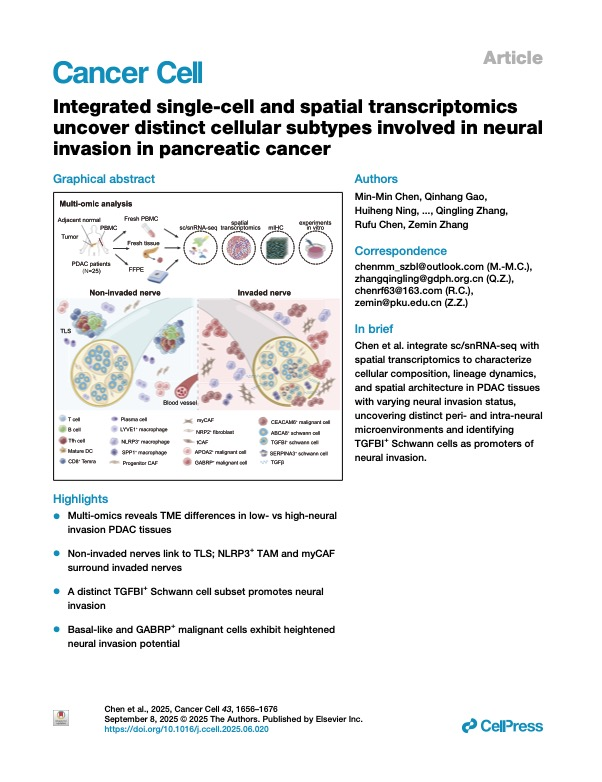
\includegraphics[width=\linewidth]{Figures/Cover.jpg}
      \small{
      \textit{Cancer Cell}, Volume 43, Issue 9, p1656--1676.e10, Sept. 08, 2025

      DOI: 10.1016/j.ccell.2025.06.020
      }
    \end{column}
    \begin{column}{0.5\textwidth}
      \vspace{0pt}
      \small
      \textbf{Title}\\
      Integrated single-cell and spatial transcriptomics uncover distinct cellular subtypes involved in neural invasion in pancreatic cancer 
      \\[0.5cm]
      \textbf{Study at a glance}
      \begin{itemize}\itemsep2pt
        \item Human PDAC cohort with resected tumors.
        \item Integrated sc/snRNA-seq and spatial transcriptomics.
        \item Compare low- vs high-NI regions in the pancreas.
        \item Identify Schwann cells, stromal, immune and malignant
              subtypes associated with NI.
      \end{itemize}
    \end{column}
  \end{columns}
\end{frame}

\section{Research Background}

\begin{frame}{Cancer as a Disease of the Microenvironment}
  \begin{itemize}
    \item Traditional view: Cancer was considered mainly a disease of \textbf{malignant cells}.
    \item Modern view: Cancer is a complex ecosystem (Tumor microenvironment, \textbf{TME}) involving
      \begin{itemize}
        \item Tumor cells
        \item Stromal cells (fibroblasts, endothelial cells, etc.)
        \item Immune cells
        \item \textbf{Nerves and the nervous system}
      \end{itemize}
    \item The nervous system regulates
      \begin{itemize}
        \item Organ development
        \item Tissue homeostasis
        \item Immune function
      \end{itemize}
    \item Increasing evidence: nerves actively participate in
      \begin{itemize}
        \item Tumor growth and survival
        \item \textbf{Invasion and metastasis}
        \item Therapy resistance
      \end{itemize}
  \end{itemize}
\end{frame}

\begin{frame}{Neural Involvement in Cancer}
  \begin{itemize}
    \item Autonomic and sensory nerves can
      \begin{itemize}
        \item Promote tumor proliferation and invasion
        \item Shape the local immune microenvironment
        \item Modulate responses to chemo- and radiotherapy
      \end{itemize}
    \item Some studies also suggest \textbf{anti-tumor} roles of certain neural components.
    \item However, our knowledge is still limited:
      \begin{itemize}
        \item Which specific neural and non-neural cell types are involved?
        \item How do they interact within and around nerves?
        \item How do these interactions drive disease progression?
      \end{itemize}
    \item \(\Rightarrow\) Tumor-associated nerves represent a \textbf{critical but poorly understood} niche.
  \end{itemize}
\end{frame}

\begin{frame}{Neural (Perineural) Invasion}
  \begin{itemize}
    \item \textbf{Neural invasion / perineural invasion (NI/PNI):}
      \begin{itemize}
        \item Presence of \textbf{tumor cells within or around nerve structures}
        \item Involving epineurium, perineurium, or endoneurium
      \end{itemize}
    \item Common histopathological definitions:
      \begin{itemize}
        \item Tumor cells identified \textbf{inside the nerve sheath}, or
        \item Tumor cells surrounding a large proportion of the nerve circumference
      \end{itemize}
    \item NI is a form of \textbf{local tumor spread}, distinct from:
      \begin{itemize}
        \item Vascular invasion (via blood vessels)
        \item Lymphatic invasion (via lymphatic vessels)
      \end{itemize}
    \item Observed in many solid tumors:
      \begin{itemize}
        \item \textbf{Pancreatic}, prostate, head and neck, colorectal, etc.
      \end{itemize}
  \end{itemize}
\end{frame}

\begin{frame}{Basic Features and Clinical Impact of NI}
  \begin{columns}[T,onlytextwidth]
    \begin{column}{0.58\textwidth}
      \begin{itemize}
        \item \textbf{Morphological features:}
          \begin{itemize}
            \item Tumor cells tracking along nerves or clustering around nerve bundles
            \item Can involve small intrapancreatic nerves or larger extrapancreatic nerves
          \end{itemize}
        \item \textbf{Biological implications:}
          \begin{itemize}
            \item Provides a \textbf{low-resistance path} for local tumor spread
            \item Allows tumor cells to reach distant sites along nerve routes
            \item Associated with nerve remodeling and inflammation
          \end{itemize}
      \end{itemize}
    \end{column}
    \begin{column}{0.4\textwidth}
      \begin{figure}
        \centering
        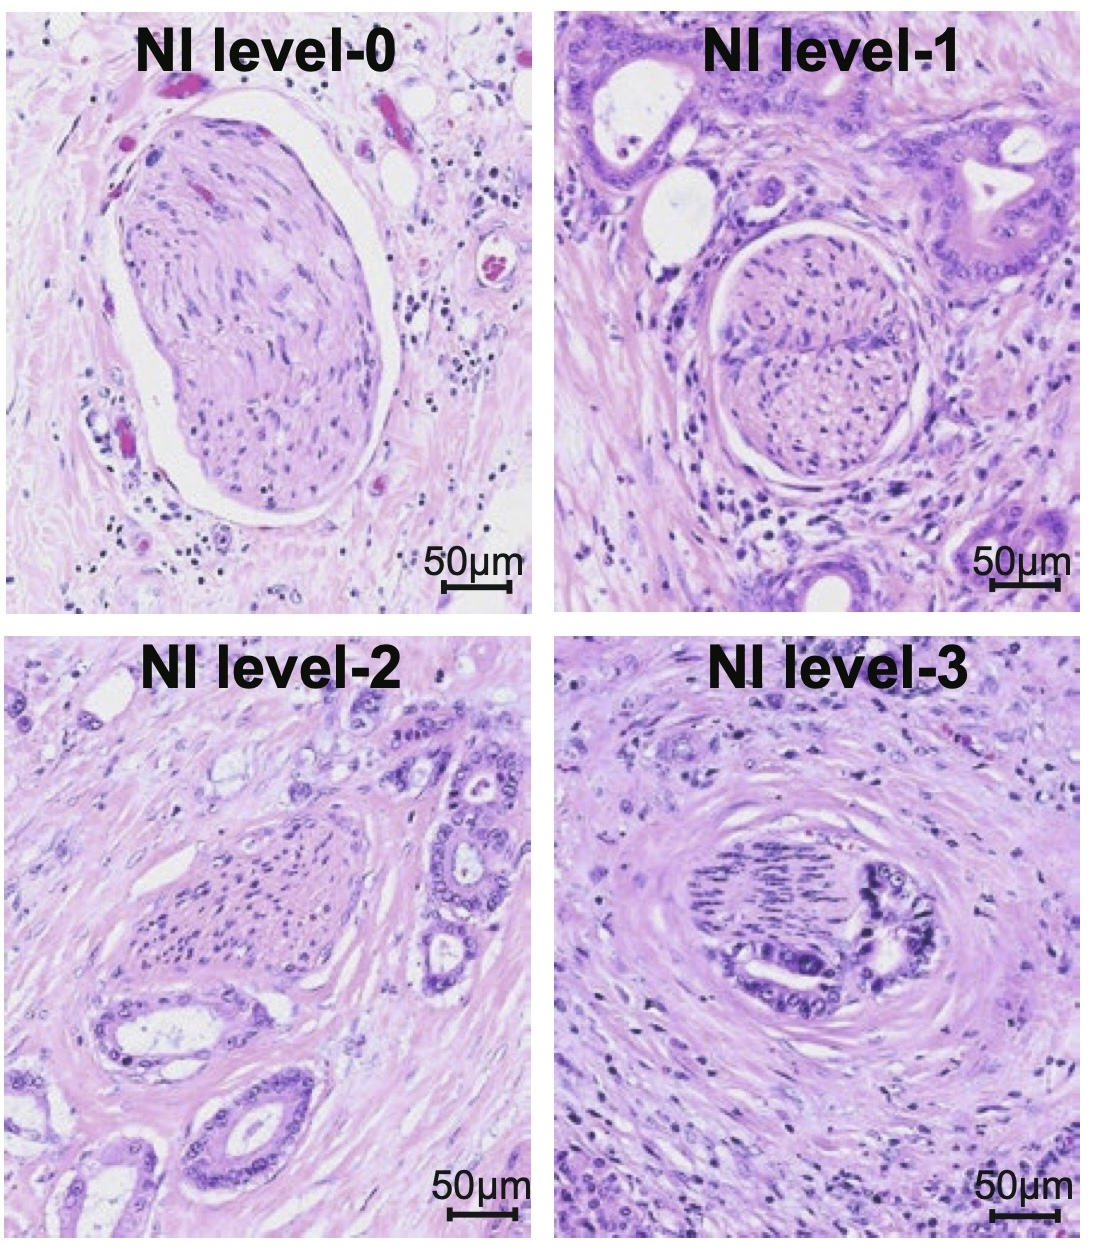
\includegraphics[width=\linewidth]{Figures/S1A.jpg}
      \end{figure}
    \end{column}
  \end{columns}
  \begin{itemize}
    \item \textbf{Clinical consequences:}
  \begin{itemize}
    \item Independent predictor of poor prognosis in several cancers
    \item Contributes to \textbf{local recurrence} and \textbf{distant metastasis}
    \item Strongly linked to \textbf{cancer-related neuropathic pain}
  \end{itemize}
  \end{itemize}
\end{frame}



\begin{frame}{Neural Invasion in Pancreatic Ductal Adenocarcinoma (PDAC)}
  \begin{itemize}
    \item The pancreas is a \textbf{highly innervated} organ.
    \item PDAC shows extremely high rates of NI/PNI:
      \begin{itemize}
        \item Often reported in \textbf{\(\sim\)80--100\%} of resected tumors
      \end{itemize}
    \item NI in PDAC is:
      \begin{itemize}
        \item An \textbf{independent} adverse prognostic factor
        \item Associated with \textbf{local recurrence} along nerve plexuses
        \item Related to \textbf{distant metastasis} and \textbf{shortened survival}
      \end{itemize}
    \item Clinically important symptoms:
      \begin{itemize}
        \item Severe abdominal and back pain attributed to nerve involvement
      \end{itemize}
    \item \(\Rightarrow\) Understanding NI in PDAC is crucial for
      \begin{itemize}
        \item Better risk stratification and prognosis
        \item Development of \textbf{nerve-targeted} therapeutic strategies
      \end{itemize}
  \end{itemize}
\end{frame}

\begin{frame}{Mechanistic View: How Does NI Occur?}
  \begin{itemize}
    \item \textbf{Bidirectional crosstalk} between tumor cells and nerves:
      \begin{itemize}
        \item Tumor cells secrete neurotrophic factors and chemokines
        \item Nerves release growth factors and neurotransmitters
      \end{itemize}
    \item Stromal and immune cells in perineural regions:
      \begin{itemize}
        \item Support tumor cell survival and migration
        \item Modulate local inflammation and pain
      \end{itemize}
    \item Conceptual model:
      \begin{itemize}
        \item Tumor cells \textbf{“hijack” neural pathways} as routes of spread
        \item Nerves are reshaped into a \textbf{pro-tumor niche}
      \end{itemize}
    \item \textbf{Knowledge gap:}
      \begin{itemize}
        \item The exact \textbf{cellular composition} of this nerve-associated niche
        \item How different cell subtypes collectively drive NI in PDAC
        \item \(\Rightarrow\) Motivates single-cell and spatial dissection in this study
      \end{itemize}
  \end{itemize}
\end{frame}

\begin{frame}{Limitations of Existing Studies on Neural Invasion}
  \begin{itemize}
    \item Previous work has focused on
      \begin{itemize}
        \item Neurotrophic factors, chemokines, axon guidance molecules
        \item \textit{In vitro} co-culture systems and animal models
      \end{itemize}
    \item These studies highlight \textbf{bidirectional signaling} between tumor cells and nerves.
    \item Stromal and immune cells are also implicated in neural invasion.
    \item However:
      \begin{itemize}
        \item Most studies examine \textbf{single molecules} or \textbf{single cell types}.
        \item There is no comprehensive map of the \textbf{cellular ecosystem} inside and around nerves.
        \item Translation of these findings to clinical practice remains limited.
      \end{itemize}
  \end{itemize}
\end{frame}

\begin{frame}{Advances in Single-Cell and Spatial Omics}
  \begin{itemize}
    \item Single-cell/single-nucleus RNA sequencing has
      \begin{itemize}
        \item Revealed diverse malignant cell states in PDAC
        \item Characterized stromal and immune cell heterogeneity
      \end{itemize}
    \item Spatial transcriptomics has
      \begin{itemize}
        \item Linked cell states to their anatomical locations
        \item Uncovered spatially organized tumor-stroma niches
      \end{itemize}
    \item Despite these advances:
      \begin{itemize}
        \item Most studies focus on \textbf{bulk tumor and stromal regions}
        \item The \textbf{nerve-associated compartment} (inside and around nerves) remains poorly characterized
      \end{itemize}
    \item \(\Rightarrow\) A systematic, spatially resolved map of nerve-associated microenvironments in PDAC is still missing.
  \end{itemize}
\end{frame}

\begin{frame}{Rationale of This Study}
  \begin{itemize}
    \item \textbf{Biological and clinical need:}
      \begin{itemize}
        \item Neural invasion is highly prevalent and clinically important in PDAC.
        \item The cellular and molecular mechanisms within nerves and perineural regions are not well defined.
      \end{itemize}
    \item \textbf{Technological opportunity:}
      \begin{itemize}
        \item Single-cell/single-nucleus RNA-seq can resolve cell types and states at high resolution.
        \item Spatial transcriptomics can preserve anatomical context, including nerve structures.
      \end{itemize}
    \item \textbf{Overall goal of the paper:}
      \begin{itemize}
        \item To integrate single-cell/single-nucleus and spatial transcriptomic data from PDAC.
        \item To delineate \textbf{distinct cellular subtypes} within nerve-associated microenvironments.
        \item To uncover how these subtypes contribute to \textbf{neural invasion} in pancreatic cancer.
      \end{itemize}
  \end{itemize}
\end{frame}

\section{Research Methods}

\begin{frame}{Research Methods Overview}
  \begin{figure}
    \centering
    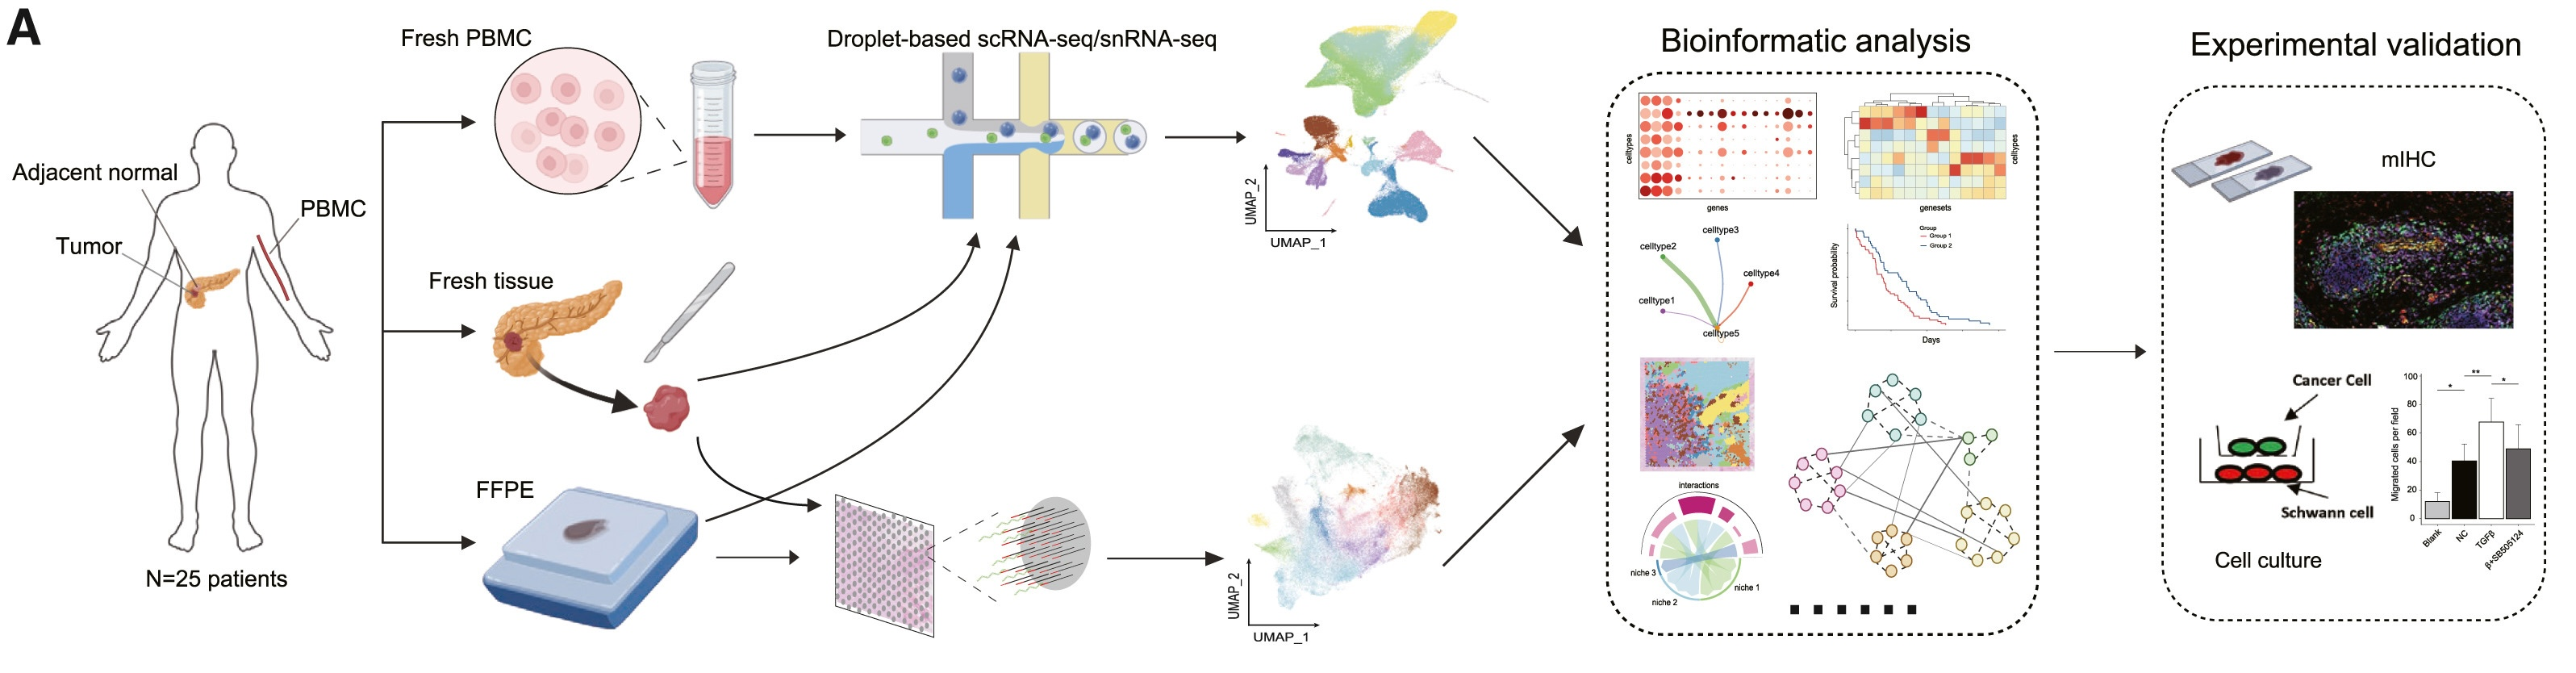
\includegraphics[width = 0.9\linewidth]{Figures/1A.jpg}
  \end{figure}
  \begin{itemize}
    \item Multi-region PDAC cohort integrating:
    \begin{itemize}
      \item Single-cell / single-nucleus RNA sequencing (sc/snRNA-seq)
      \item Spatial transcriptomics (Visium on fresh-frozen and FFPE)
      \item Histology \& multiplex immunohistochemistry / immunofluorescence
      \item \textit{In vitro} functional assays
    \end{itemize}
    \item Focus: cellular ecosystem and neural invasion (NI) in human PDAC
    \item Strategy:
    \begin{itemize}
      \item Build single-cell atlas of tumors, adjacent pancreas, and blood
      \item Map cell states in space using ST
      \item Model cell-cell communication and validate key interactions
    \end{itemize}
  \end{itemize}
\end{frame}

\begin{frame}{Patient Cohort \& Tissue Sampling}
  \begin{itemize}
    \item Fresh surgical PDAC specimens
    \begin{itemize}
      \item Primary tumor regions
      \item Adjacent non-tumor pancreas
      \item Peripheral blood (PBMCs)
      \item In total 62 samples from 25 PDAC patients
    \end{itemize}
    \item Standard histology
    \begin{itemize}
      \item H\&E staining of representative blocks
      \item Pathologist review of tumor, stroma, nerves
    \end{itemize}
    \item Neural invasion (NI) assessment
    \begin{itemize}
      \item Identification of perineural invasion (PNI)
      \item Semi-quantitative NI score per case
      \item Classification into low-NI (8 patients) vs high-NI (17 patients) tumors
    \end{itemize}
  \end{itemize}
\end{frame}

\begin{frame}{sc/snRNA-seq Data Generation}
  \begin{itemize}
    \item Tissue dissociation and nuclei isolation
    \begin{itemize}
      \item Fresh tumor: single-cell suspensions for scRNA-seq
      \item Frozen / less viable tissue: nuclei for snRNA-seq
    \end{itemize}
    \item Library preparation \& sequencing
    \begin{itemize}
      \item 10x Genomics platform (scRNA-seq and snRNA-seq)
      \item Generation of gene-cell count matrices
    \end{itemize}
    \item Quality control
    \begin{itemize}
      \item Filtering low-complexity cells/nuclei
      \item Removing cells with high mitochondrial gene percentage
      \item Doublet and ambient RNA removal (standard pipelines)
    \end{itemize}
  \end{itemize}
\end{frame}

\begin{frame}{Single-Cell Data Processing \& Annotation}
  \begin{itemize}
    \item Data integration
    \begin{itemize}
      \item Batch correction across patients, tissues, sc vs sn
      \item Dimensionality reduction (PCA, UMAP)
      \item Unsupervised clustering
    \end{itemize}
    \item Major lineage annotation
    \begin{itemize}
      \item Canonical markers for T/NK, B/plasma, myeloid, CAF/fibroblast
      \item Endothelial, stellate, acinar, endocrine, ductal, Schwann cells
    \end{itemize}
    \item Malignant vs non-malignant ductal cells
    \begin{itemize}
      \item Inferred large-scale CNVs from expression profiles
      \item Definition of malignant ductal subtypes
    \end{itemize}
    \item Subclustering
    \begin{itemize}
      \item Finer states within tumor, immune, stromal, and Schwann cells
    \end{itemize}
  \end{itemize}
\end{frame}

\begin{frame}{Single-Cell Data Processing \& Annotation}
  \begin{figure}
    \centering
    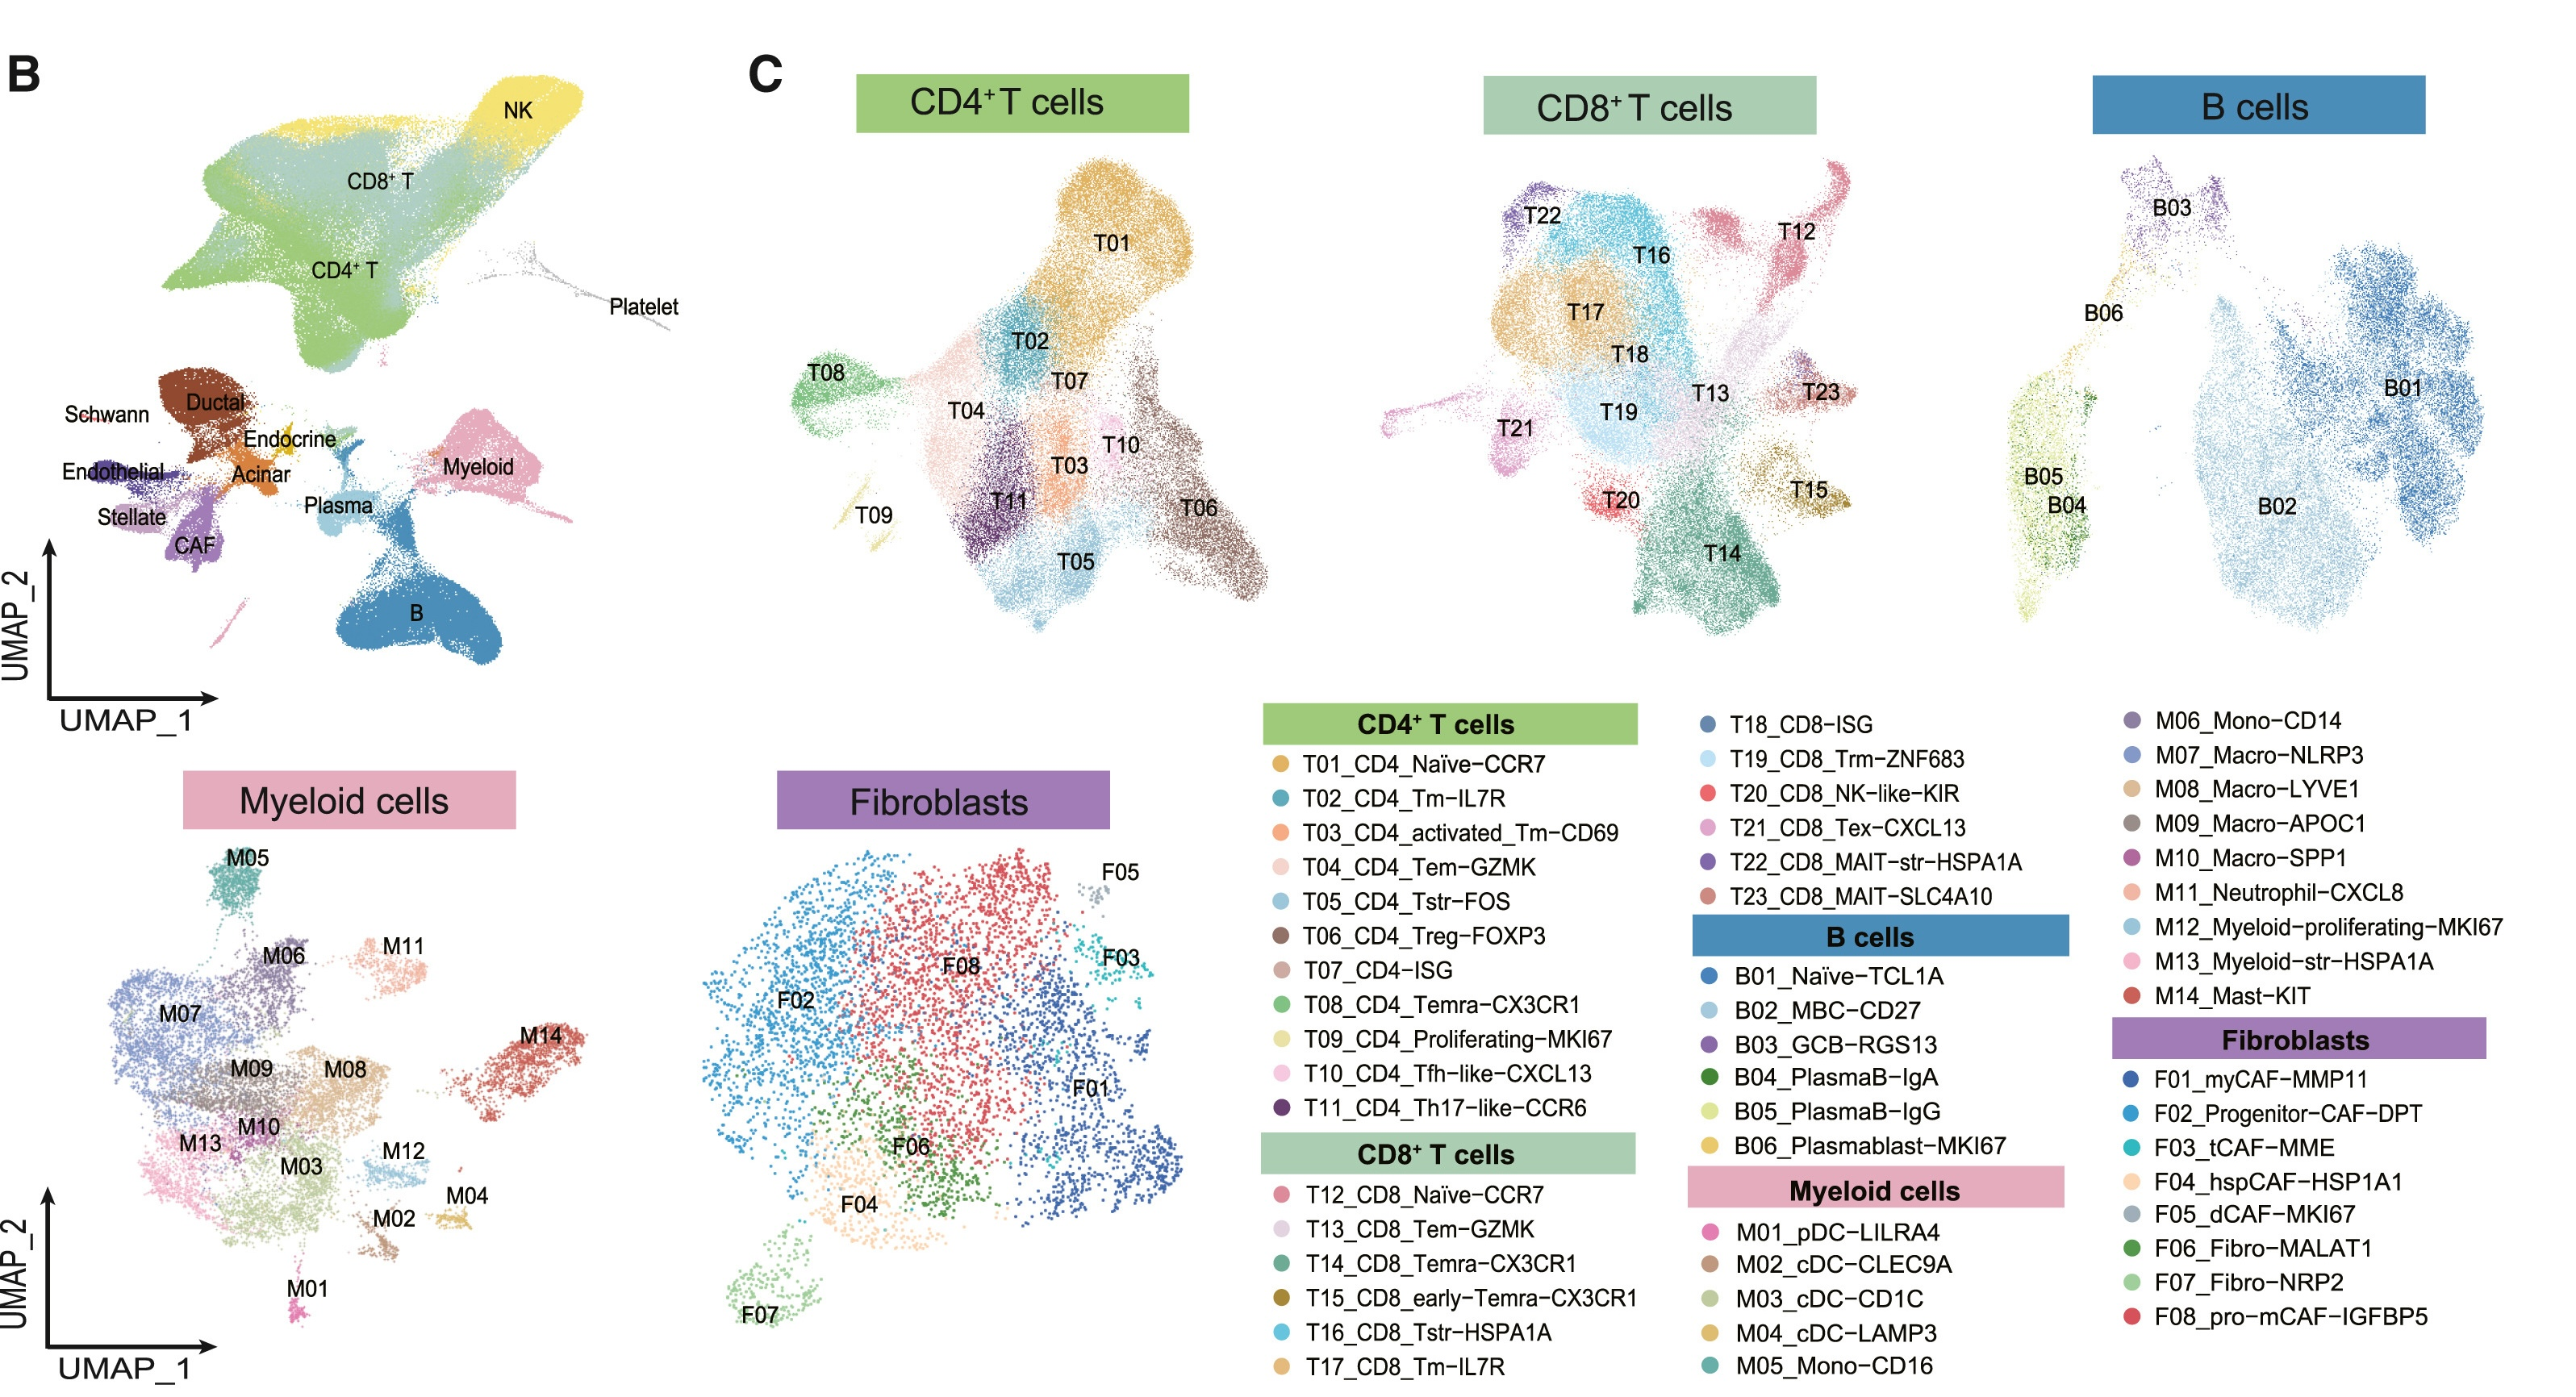
\includegraphics[width = 0.9\linewidth]{Figures/1B&C.jpg}
  \end{figure}
  \begin{itemize}
    \item B: Data integration and major lineage annotation
    \item C: Subclustering within each major lineage 
  \end{itemize}
\end{frame}

\begin{frame}{Spatial Transcriptomics}
  \begin{itemize}
    \item Platforms \& samples
    \begin{itemize}
      \item 10x Visium on fresh-frozen tissue sections
      \item CytAssist-enabled Visium on FFPE sections
      \item Adjacent H\&E sections for morphological annotation
    \end{itemize}
    \item ST data processing
    \begin{itemize}
      \item Alignment to reference genome, spot-level count matrices
      \item QC, normalization, dimensionality reduction, clustering
    \end{itemize}
    \item Cell-type deconvolution
    \begin{itemize}
      \item Projection of sc/snRNA-seq signatures onto ST spots
      \item Identification of spatial ``niches'' enriched for specific
            malignant, immune, CAF, and Schwann subtypes
    \end{itemize}
  \end{itemize}
\end{frame}

\begin{frame}{Spatial Transcriptomics}
  \begin{figure}
    \centering
    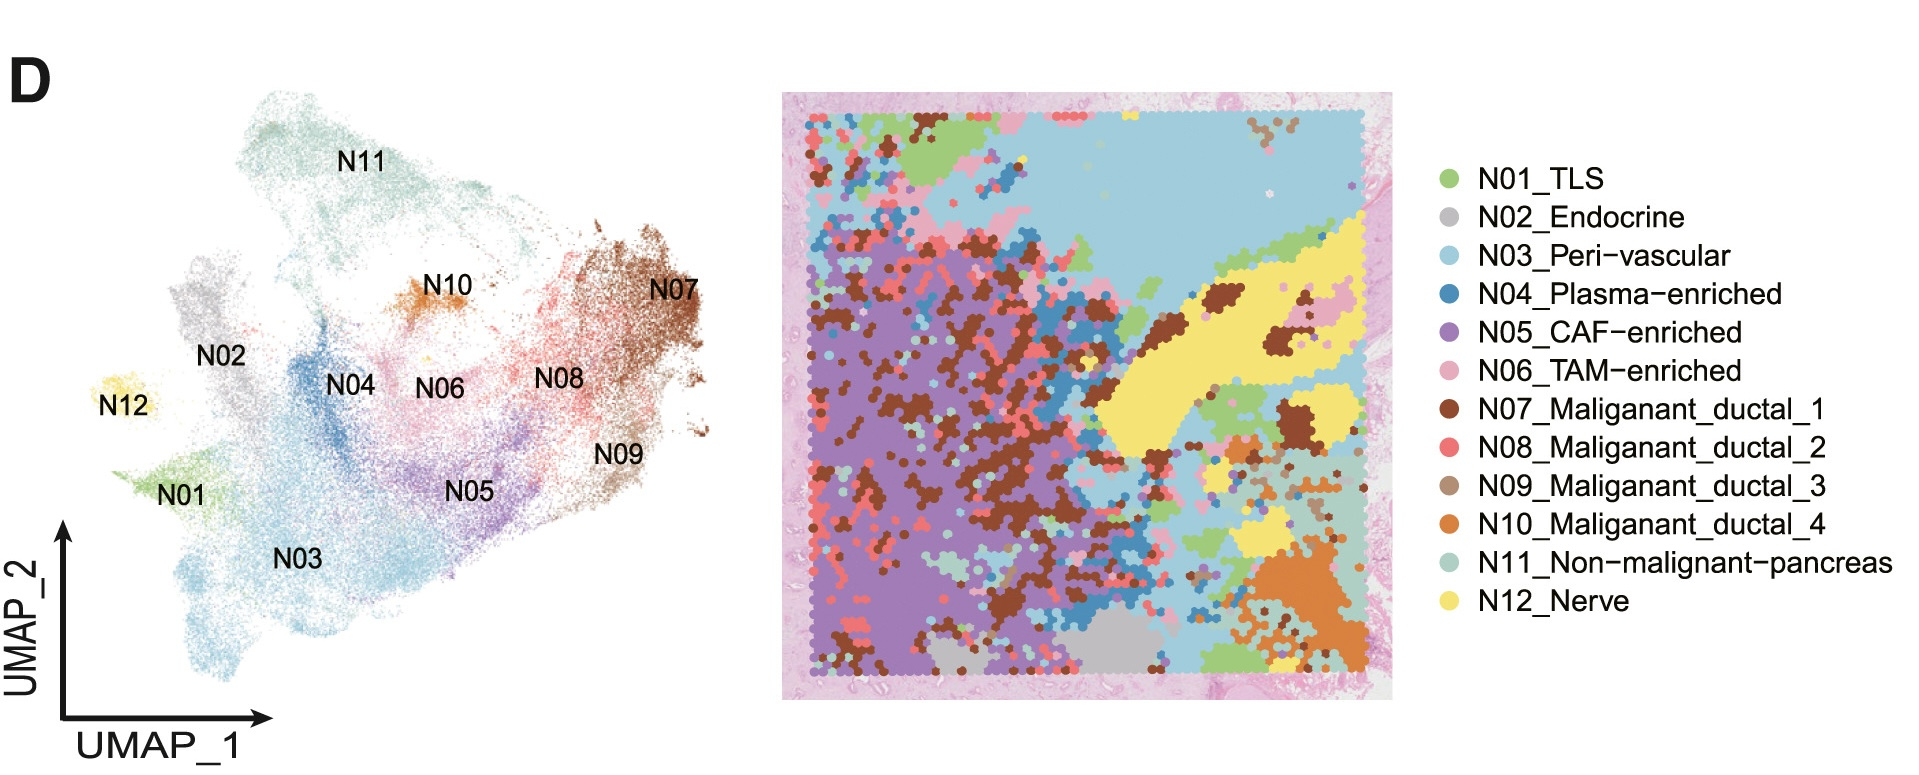
\includegraphics[width = 0.9\linewidth]{Figures/1D.jpg}
  \end{figure}
  \begin{itemize}
    \item UMAP plots showing spatial niches clustering based on gene expression of the spots (left). Mapping of spatial niches in a representative sample PA\#98 (right).
  \end{itemize}
\end{frame}

\begin{frame}{NI-Focused Spatial Analyses}
  \begin{columns}[T,onlytextwidth]
    \begin{column}{0.6\textwidth}
      \begin{itemize}
        \item Nerve annotation
          \begin{itemize}
            \item Pathologists labeled nerve bundles on H\&E (Top)
            \item Classification: invaded vs non-invaded nerves
            \item Black arrow indicates a magnified field displaying invading cancer cells 
            \item Deconvolution-based Schwann abundance around nerves (Bottom)
          \end{itemize}
        \item Distance-based analysis
          \begin{itemize}
            \item ST spots grouped by distance to nerves
            (juxta-neural rings, peri-neural regions)
            \item Comparison of cell-type composition and gene signatures around invaded vs non-invaded nerves
          \end{itemize}
      \end{itemize}
    \end{column}
    \begin{column}{0.38\textwidth}
      \begin{figure}
        \centering
        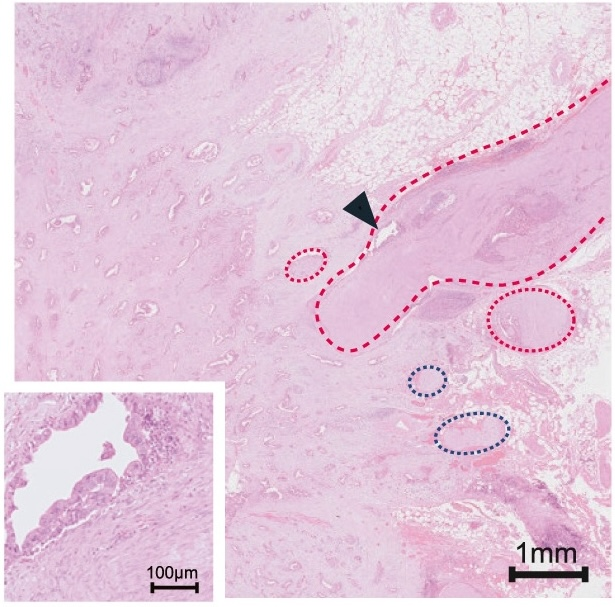
\includegraphics[width = 0.8\linewidth]{Figures/1El.jpg}
      \end{figure}
      \begin{figure}
        \centering
        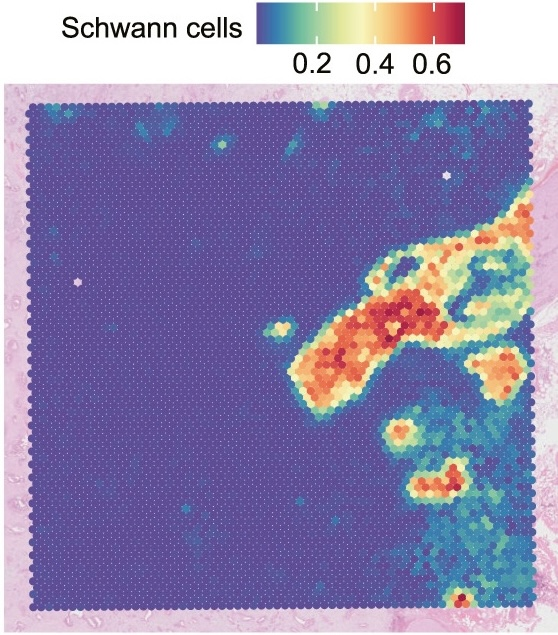
\includegraphics[width = 0.8\linewidth]{Figures/1Er.jpg}
      \end{figure}
    \end{column}
  \end{columns}
\end{frame}

\begin{frame}{NI-Focused Spatial Analyses}
  \begin{figure}
    \centering
    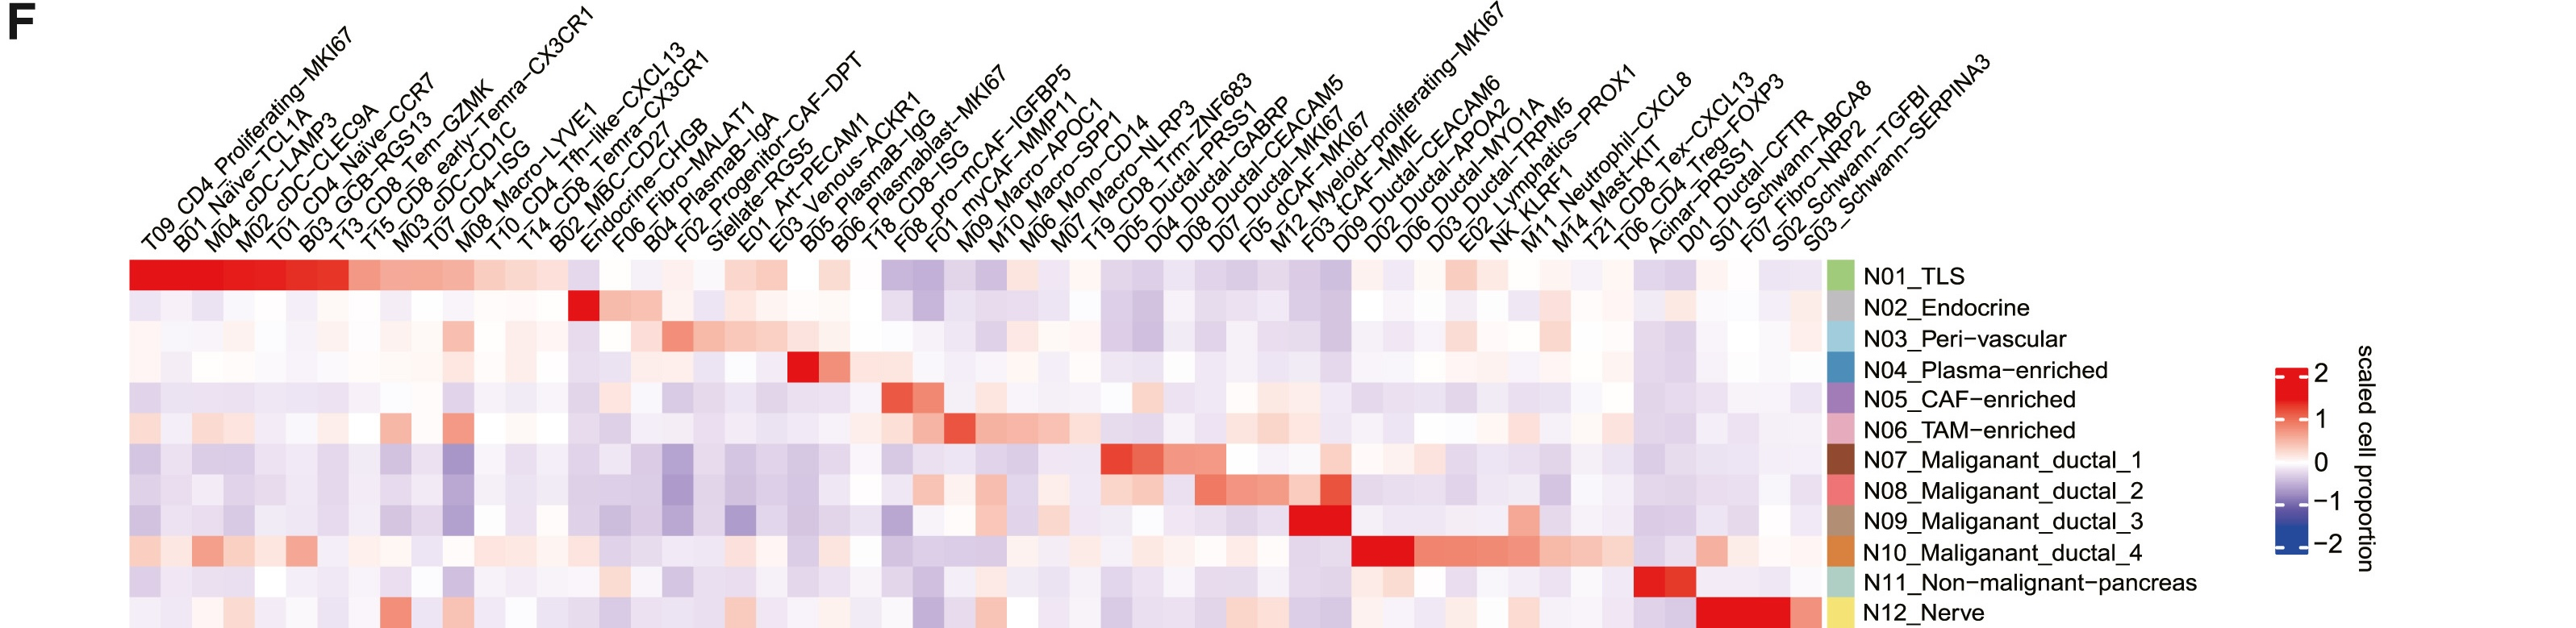
\includegraphics[width = 0.95\linewidth]{Figures/1F.jpg}
  \end{figure}
  \begin{columns}[T,onlytextwidth]
    \begin{column}{0.7\textwidth}
      \begin{itemize}
        \item Integration with tumor regions
        \begin{itemize}
          \item Mapping of tumor, stromal, and TLS-like niches
          \item Analysis of nerve-tumor interfaces and associated cell states
          \item Heatmap of cell proportions per spatial niche (top)
          \item Schwann cells predominantly located in the N12\_Nerve niche (right)
        \end{itemize}
      \end{itemize}
    \end{column}
    \hspace{-1cm}
    \begin{column}{0.28\textwidth}
      \begin{figure}
        \raggedright 
        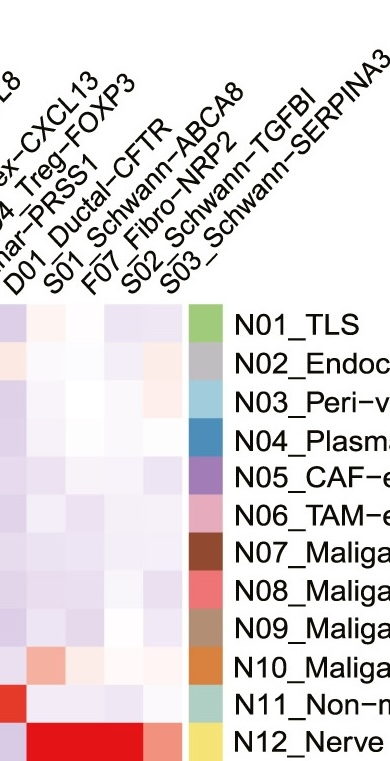
\includegraphics[width = 0.6\linewidth]{Figures/1Flrg.jpg}
      \end{figure}
    \end{column}
  \end{columns}
\end{frame}

\begin{frame}{Cell-Cell Communication \& Multi-Omics Integration}
  \begin{itemize}
    \item Ligand-receptor inference (sc/snRNA-seq)
    \begin{itemize}
      \item Modeling signaling between malignant cells, CAFs, myeloid cells,
            T cells, and Schwann subsets
      \item Focus on pathways related to neural remodeling and immunity
    \end{itemize}
    \item Cytokine signaling into Schwann cells
    \begin{itemize}
      \item Estimation of pathway activities (e.g. TGF-\(\upbeta\))
      \item Association with distinct Schwann cell states
    \end{itemize}
    \item Spatial interaction modelling
    \begin{itemize}
      \item Construction of spatial networks from ST data
      \item Quantifying co-localization and influence across niches
    \end{itemize}
  \end{itemize}
\end{frame}

\begin{frame}{Imaging Validation \& Functional Assays}
  \begin{columns}[T,onlytextwidth]
    \begin{column}{0.65\textwidth}
      \begin{figure}
        \centering
        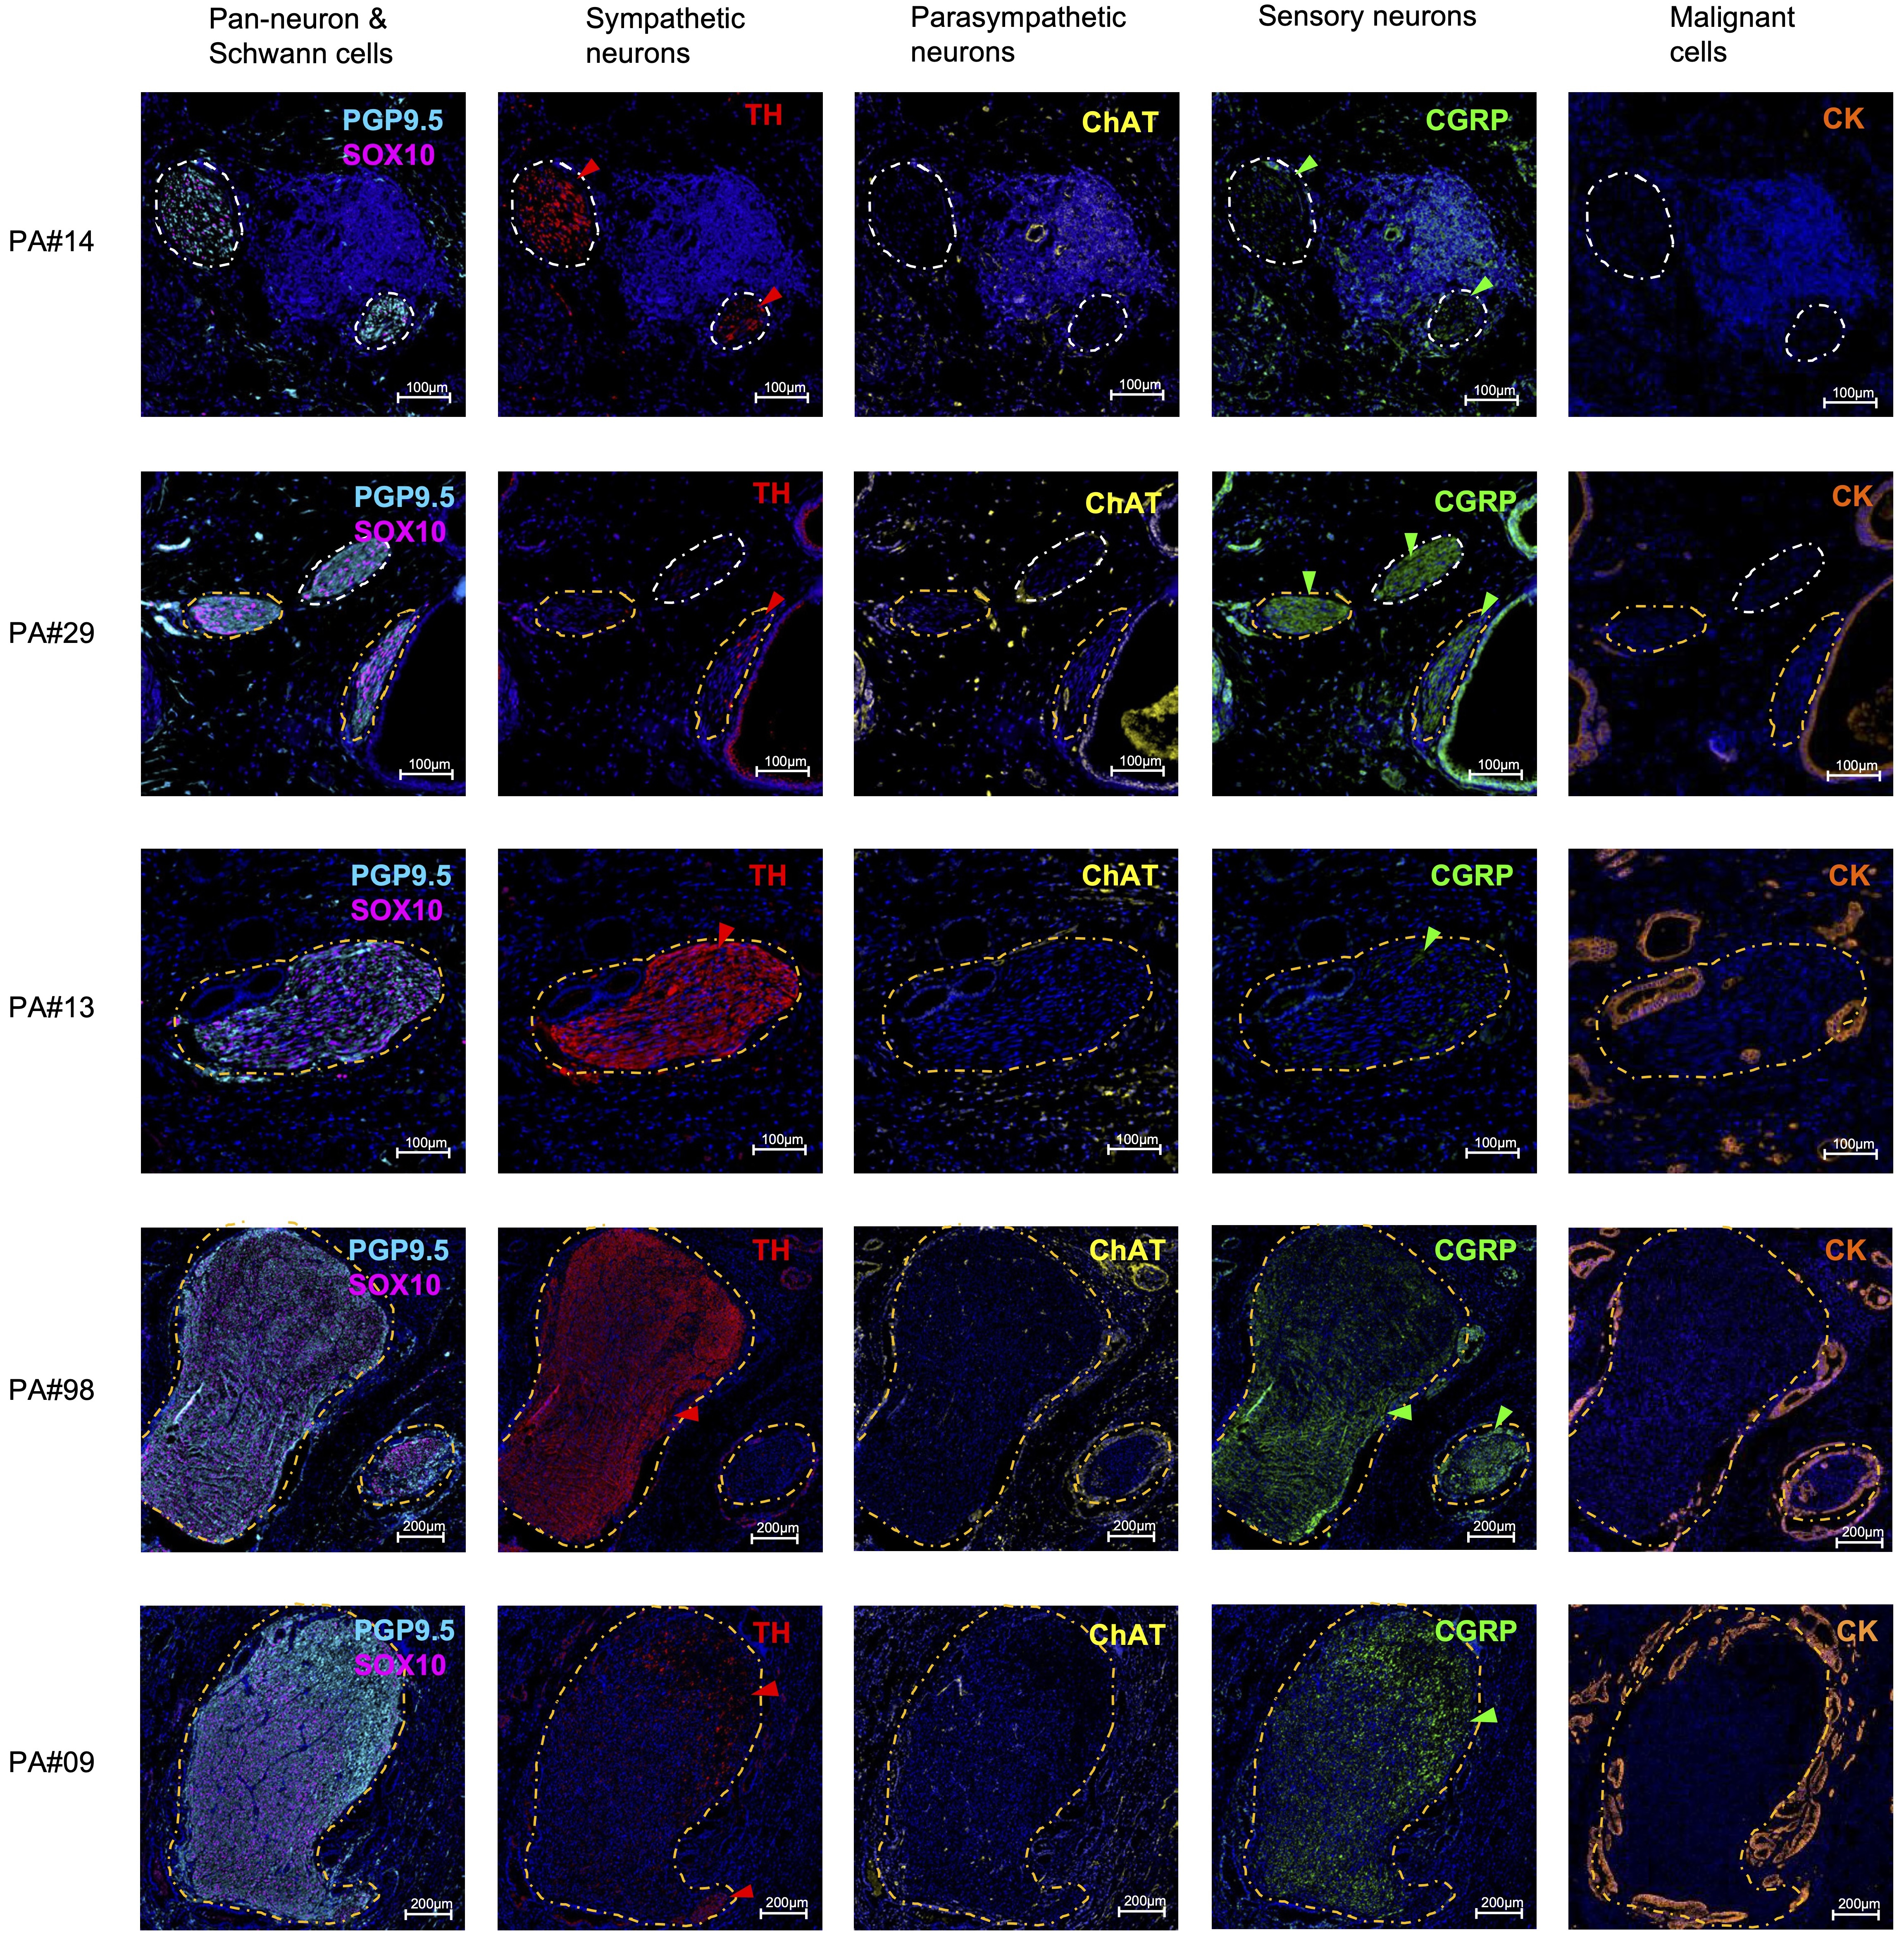
\includegraphics[width = 0.9\linewidth]{Figures/S2A.jpg}
      \end{figure} 
    \end{column}
    \begin{column}{0.34\textwidth}
      \begin{itemize}
        \item Multiplex IHC / IF
        \item Gold dashed lines indicate invaded nerves, while white dashed lines indicate non-invaded nerves
        \item Nerve bundles comprised both TH\(^+\) sympathetic and CGRP\(^+\) sensory neurons, whereas ChAT\(^+\) parasympathetic neurons were relatively rare
      \end{itemize}
    \end{column}
  \end{columns}
  \begin{itemize}
    \item Both sympathetic-dominant nerves and sensory-dominant nerves were found to be susceptible to invasion
  \end{itemize}
\end{frame}

\begin{frame}{Imaging Validation \& Functional Assays}
  \begin{itemize}
    \item \textit{In vitro} Schwann cell assays
    \begin{itemize}
      \item Human Schwann cell line treated with TGF-\(\upbeta\)
            \(\pm\) TGF-\(\upbeta\) receptor inhibitor
      \item Transcriptomic comparison with \textit{in vivo} Schwann states
    \end{itemize}
    \item Tumor cell migration assays
    \begin{itemize}
      \item PDAC cells exposed to different Schwann-conditioned media
      \item Time-lapse imaging to measure migration velocity
    \end{itemize}
  \end{itemize}
\end{frame}

\begin{frame}{Statistical Analysis}
  \begin{itemize}
    \item Group comparisons
    \begin{itemize}
      \item Low-NI vs high-NI tumors
      \item Invaded vs non-invaded nerves
      \item Tests: mainly two-sided Wilcoxon rank-sum tests
    \end{itemize}
    \item Correlation analyses
    \begin{itemize}
      \item NI scores vs clinical/pathological variables
      \item Pearson correlation with confidence intervals
    \end{itemize}
    \item Enrichment \& pathway analysis
    \begin{itemize}
      \item Gene set enrichment for pathways (e.g. EMT, neural signaling)
      \item Diversity indices (e.g. Shannon index) for malignant subtypes
    \end{itemize}
  \end{itemize}
\end{frame}

\section{Research Results}

%==================== Part 1 ====================%
\subsection{Part 1: Malignant ductal subpopulations and neural invasion}

\begin{frame}{Part 1 Overview}
  \begin{itemize}
    \item Goal: Define malignant ductal subpopulations in PDAC and relate them to neural invasion (NI) status.
    \item Approach:
      \begin{itemize}
        \item Unsupervised clustering of ductal cells from sc/snRNA-seq.
        \item Integration with spatial transcriptomics to map malignant niches.
        \item Odds-ratio and NI-related gene scores to quantify invasion potential.
      \end{itemize}
    \item Key message:
      \begin{itemize}
        \item Specific malignant ductal subtypes (basal-like and GABRP\(^{+}\)) show heightened neural invasion potential.
      \end{itemize}
  \end{itemize}
\end{frame}

\begin{frame}{Ductal cell clustering and malignant subtypes}
  \begin{figure}
    \centering
    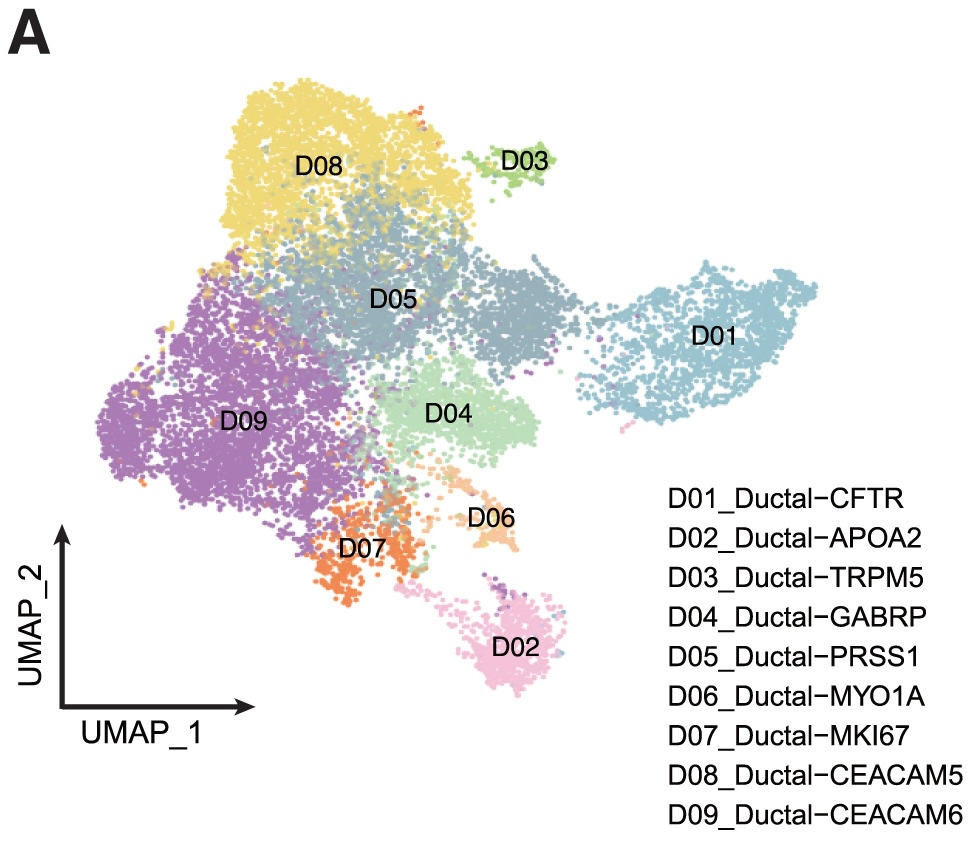
\includegraphics[width = 0.6\linewidth]{Figures/2A.jpg}
  \end{figure}
  \begin{itemize}
    \item UMAP clustering of ductal cells identified 9 subclusters (D01--D09).
  \end{itemize}
\end{frame}

\begin{frame}{Ductal cell clustering and malignant subtypes}
  \begin{figure}
    \centering
    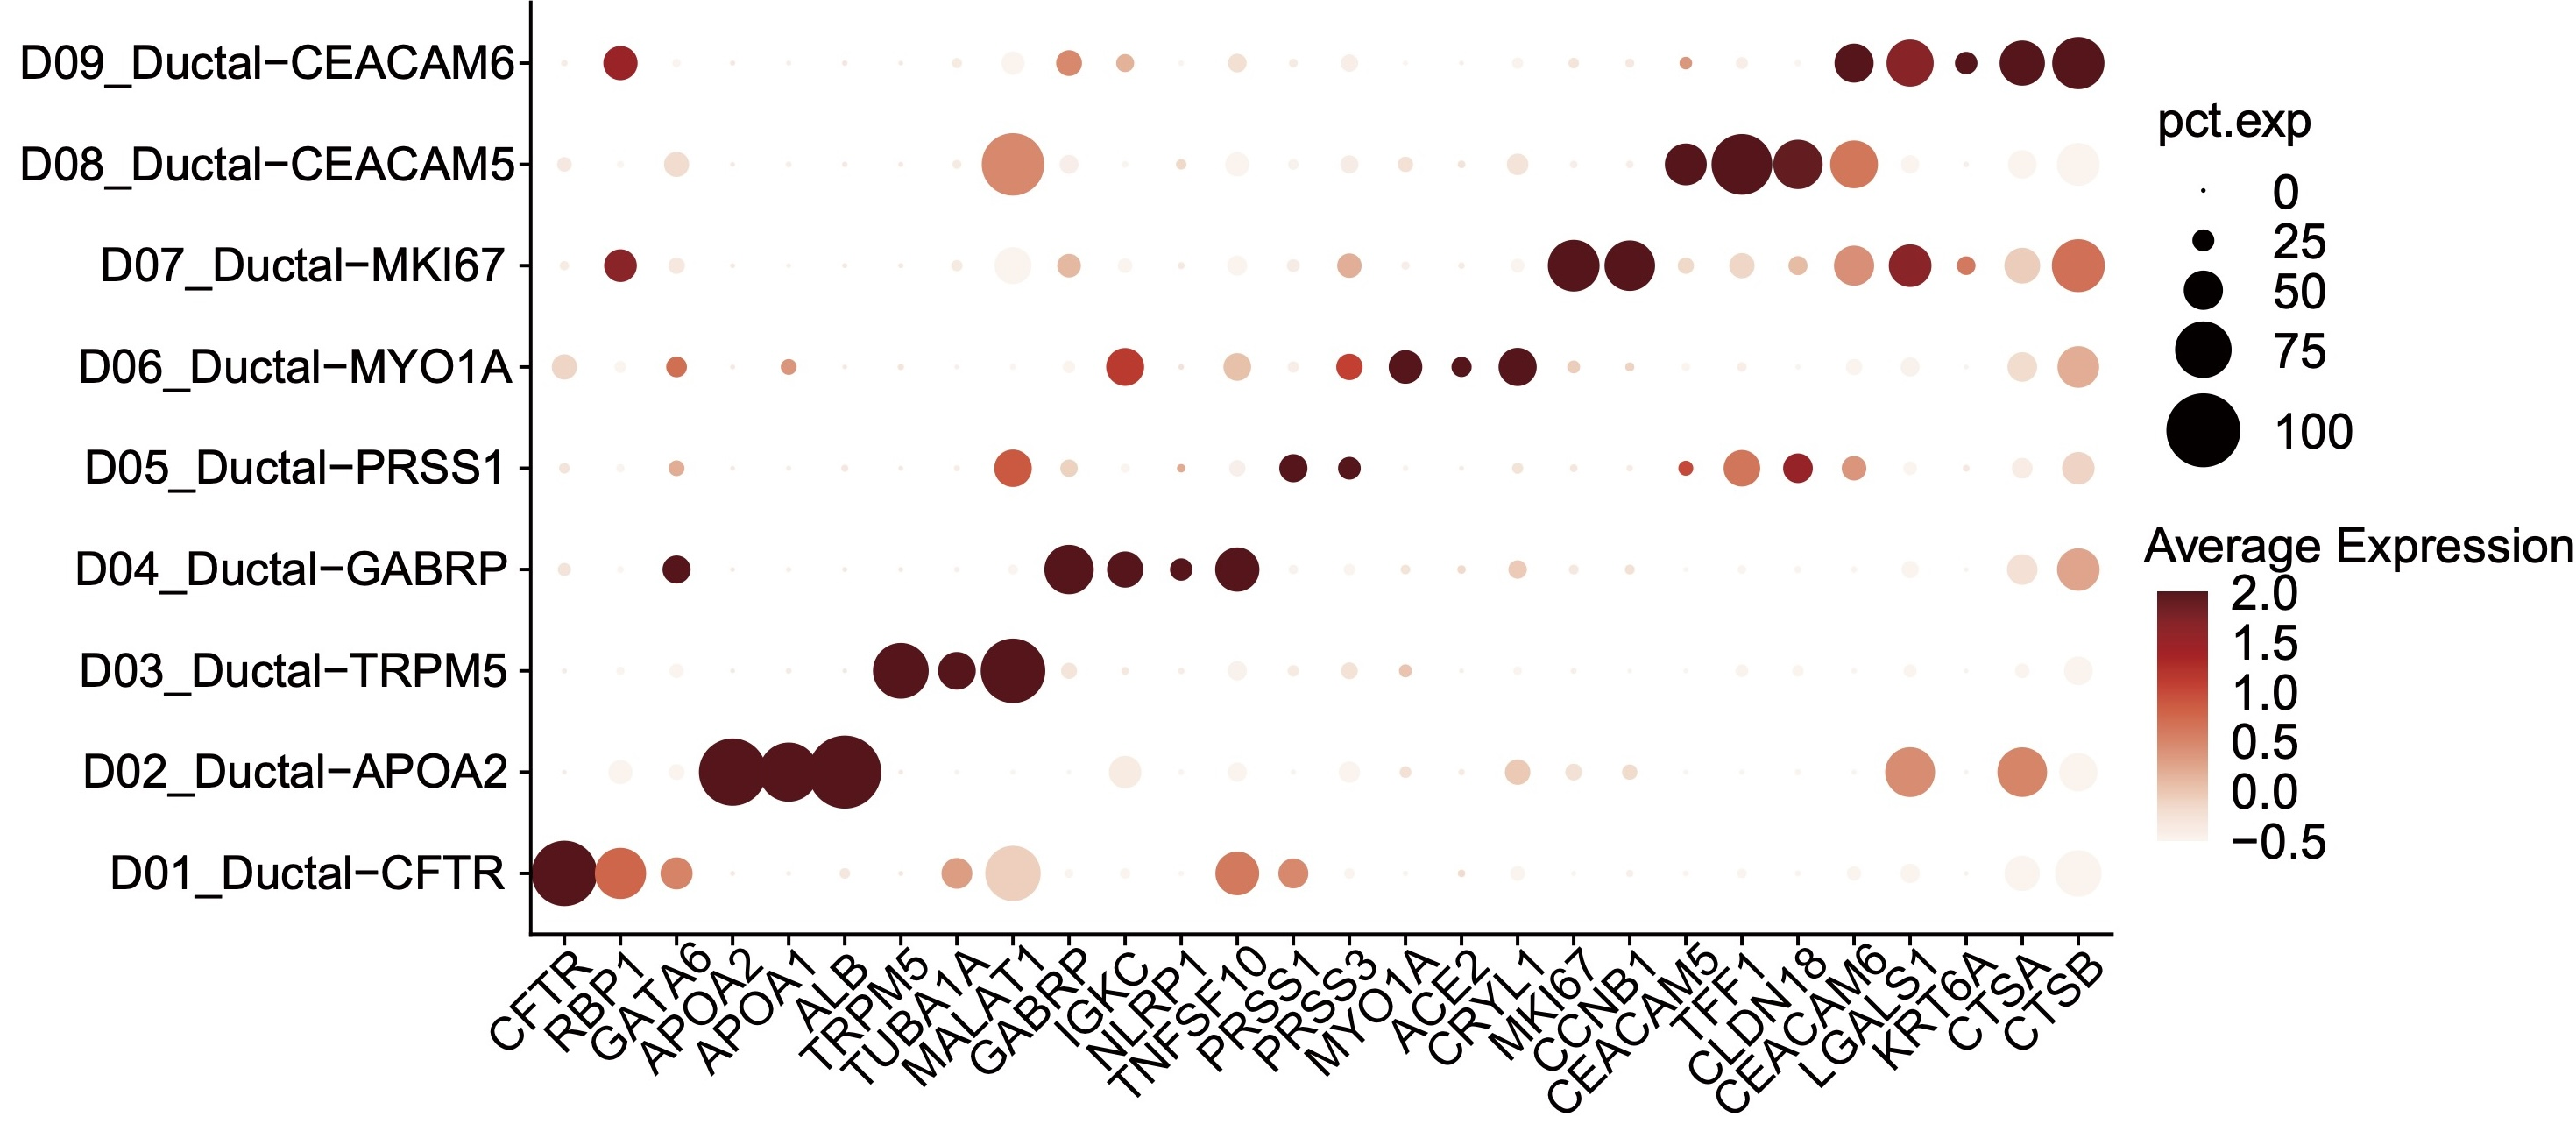
\includegraphics[width = 0.9\linewidth]{Figures/S2C.jpg}
  \end{figure}
  \begin{itemize}
    \item D01\_Ductal-CFTR:
      \begin{itemize}
        \item High expression of CFTR and other non-malignant ductal genes.
        \item Very low CNV burden \(\Rightarrow\) likely normal ductal cells.
      \end{itemize}
  \end{itemize}
\end{frame}

\begin{frame}{Ductal cell clustering and malignant subtypes}
  \begin{itemize}
    \item D02--D09: tumor ductal subpopulations with diverse CNV patterns
    \item Alignment to bulk PDAC molecular classes:
  \end{itemize}
  \begin{columns}[T,onlytextwidth]
    \begin{column}{0.5\textwidth}
      \begin{figure}
        \centering
        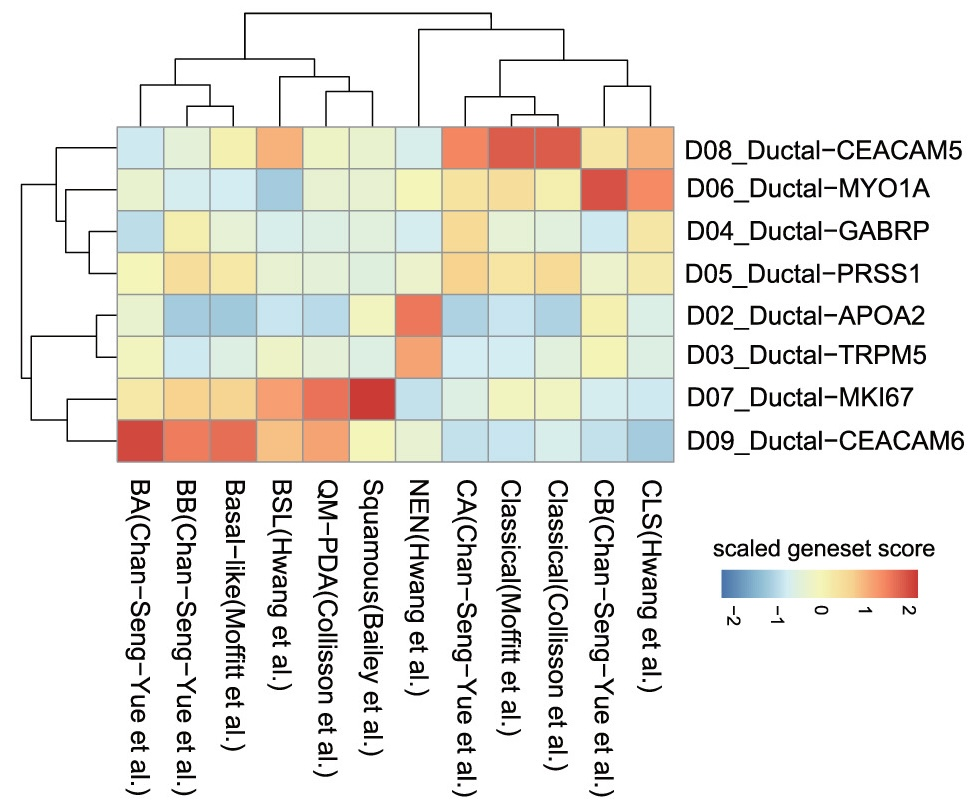
\includegraphics[width = 0.9\linewidth]{Figures/2B.jpg}
      \end{figure}
    \end{column}
    \begin{column}{0.5\textwidth}
      \begin{itemize}
        \item D08\_Ductal-CEACAM5: ``classical'' subtype.
        \item D09\_Ductal-CEACAM6: ``basal-like'' subtype.
        \item D04\_Ductal-GABRP, D05\_Ductal-PRSS1: intermediate (mixed signatures).
        \item D02\_Ductal-APOA2: neuroendocrine-like program.
      \end{itemize}
    \end{column}
  \end{columns}
\end{frame}

\begin{frame}{Ductal cell clustering and malignant subtypes}
  \begin{itemize}
    \item Deconvolute ST data to position the spots within which the proportion of a distinct malignant ductal subtype exceeded 80\%
  \end{itemize}
  \begin{columns}[T,onlytextwidth]
    \begin{column}{0.5\textwidth}
      \begin{figure}
        \centering
        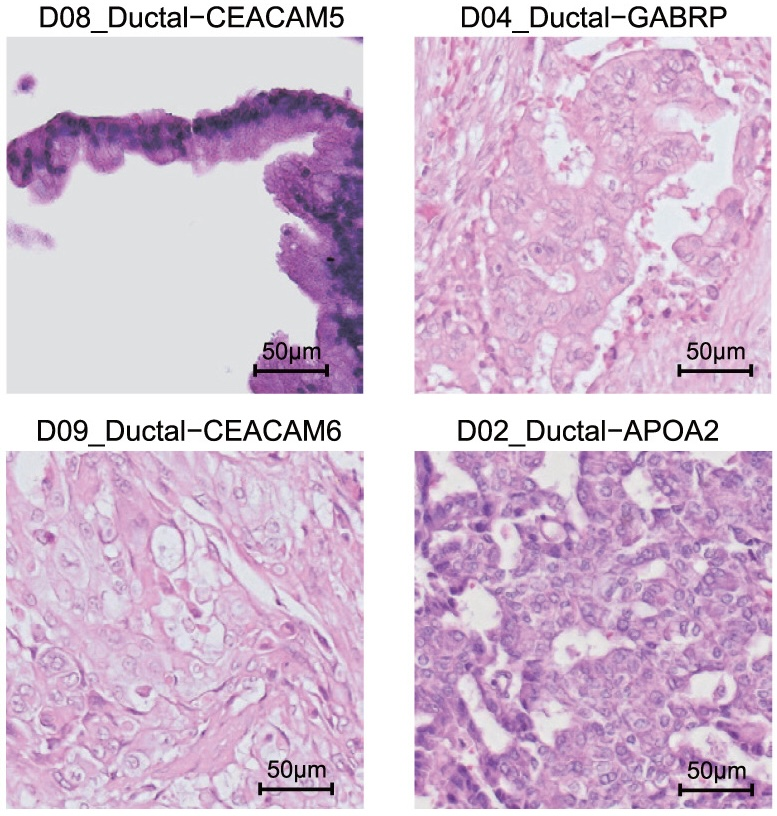
\includegraphics[width = 0.9\linewidth]{Figures/2C.jpg}
      \end{figure}
    \end{column}
    \begin{column}{0.5\textwidth}
      \begin{itemize}
        \item D08: Tubular or elongated gland phenotype (``classical'')
        \item D09: Sheets of non-glandular, large pleomorphic and anaplastic cells (``basal-like'')
        \item D04: Ill-defined glands consisting of anaplastic cells with prominent nuclear atypia (intermediate)
        \item D02: Abundant eosinophilic cytoplasm, round and regular nuclei without prominent nucleoli (neuroendocrine-like)
      \end{itemize}
    \end{column}
  \end{columns}
\end{frame}

\begin{frame}{Association of malignant subtypes with NI status}
  \begin{itemize}
    \item Used odds ratios (ORs) and ST deconvolution to compare low-NI vs high-NI samples.
  \end{itemize}
  \begin{figure}
    \centering
    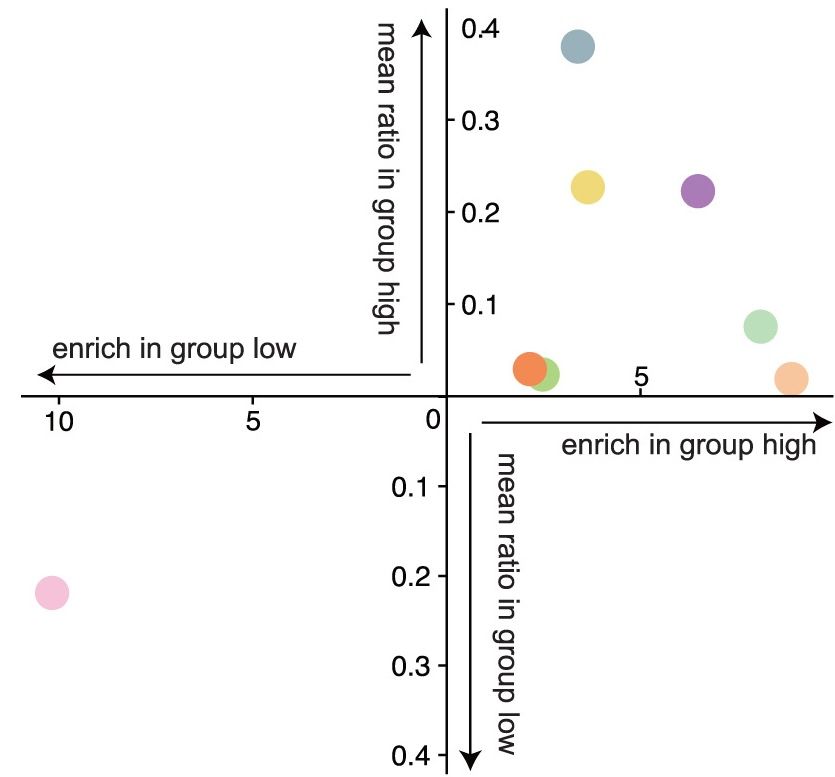
\includegraphics[width = 0.5\linewidth]{Figures/2D.jpg}
  \end{figure}
\end{frame}

\begin{frame}{Association of malignant subtypes with NI status}
  \begin{itemize}
    \item Low-NI group:
      \begin{itemize}
        \item Enrichment of D02\_Ductal-APOA2 (neuroendocrine-like).
        \item Malignant\_ductal\_4 niche (rich in D02) more prevalent.
        \item Lower NI-related gene scores in these cells.
      \end{itemize}
  \end{itemize}
  \begin{figure}
    \centering
    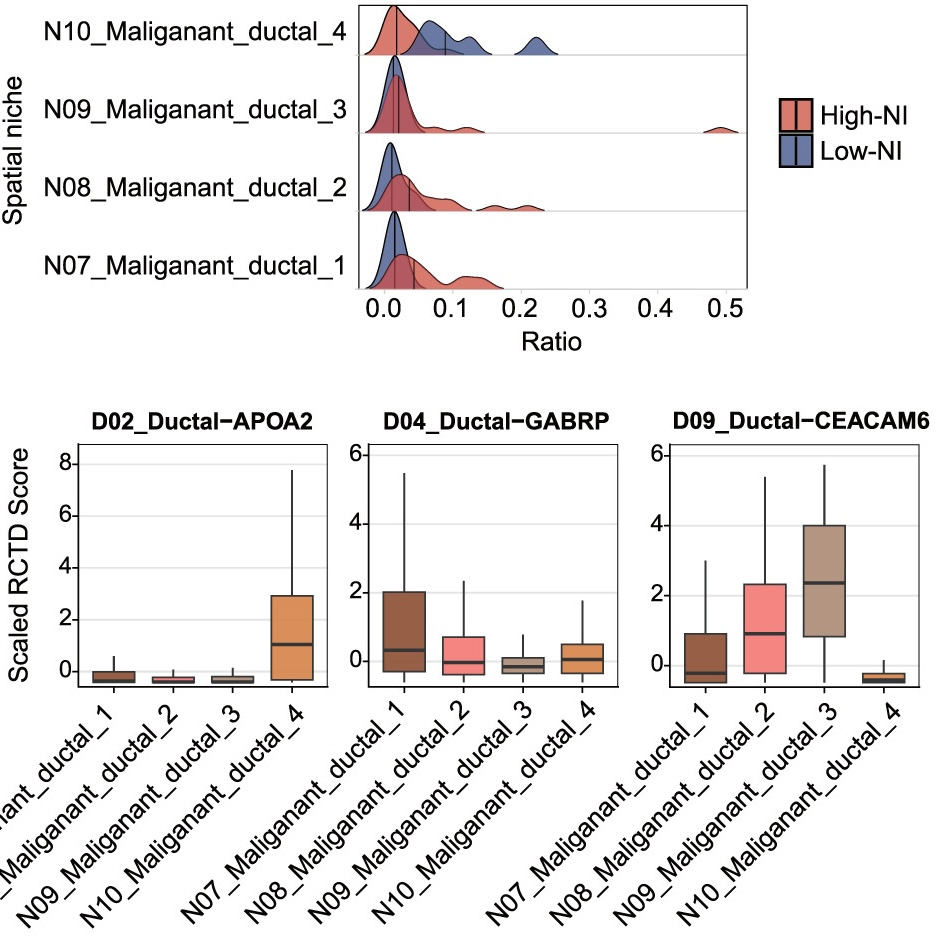
\includegraphics[width = 0.5\linewidth]{Figures/2E&F.jpg}
  \end{figure}
\end{frame}

\begin{frame}{Association of malignant subtypes with NI status}
  \begin{itemize}
    \item \textbf{D02\_Ductal-APOA2: A less invasive, neuroendocrine-like subtype}
    \item Expresses \textbf{low levels} of neural input ligands and receptors   
          
          \(\Rightarrow\) Self-sufficient neuronal signaling likely \textbf{does not} explain its low invasiveness

    \item Shows \textbf{specific upregulation of lipid metabolism genes} (APOA2, APOA1, ALB)  and enrichment of pathways:

          \(\Rightarrow\) Indicates \textbf{active cholesterol metabolism} and potential \textbf{steroid biosynthesis}, supporting a \textbf{neuroendocrine-like} feature

    \item Previous studies: \textbf{cholesterol depletion} drives a basal phenotype and \textbf{activates EMT} in PDAC  

          \(\Rightarrow\) Dysregulated lipid metabolism is associated with \textbf{metastasis}

    \item D02\_Ductal-APOA2 shows a \textbf{low EMT score}  
          \begin{itemize}
            \item Consistent with its \textbf{reduced invasiveness}
          \end{itemize}

    \item \textbf{Open question:} further experiments are needed to clarify the exact mechanisms
  \end{itemize}
\end{frame}


\begin{frame}{Association of malignant subtypes with NI status}
  \begin{itemize}
    \item High-NI group:
      \begin{itemize}
        \item Malignant subpopulations showed \textbf{lower diversity} than in the low-NI group
        \item Dominant malignant subtypes: \textbf{basal-like}, \textbf{intermediate}, and \textbf{classical}
      \end{itemize}
    \item Spatial analysis of malignant subtypes around invaded nerves
      \begin{itemize}
        \item Quantified subtype proportions within \textbf{1--5 spots} from invaded nerves
        \item \textbf{D09\_Ductal-CEACAM6} and \textbf{D04\_Ductal-GABRP} were most enriched \textbf{within 1 spot} of invaded nerves
      \end{itemize}
  \end{itemize}
  \begin{figure}
    \centering
    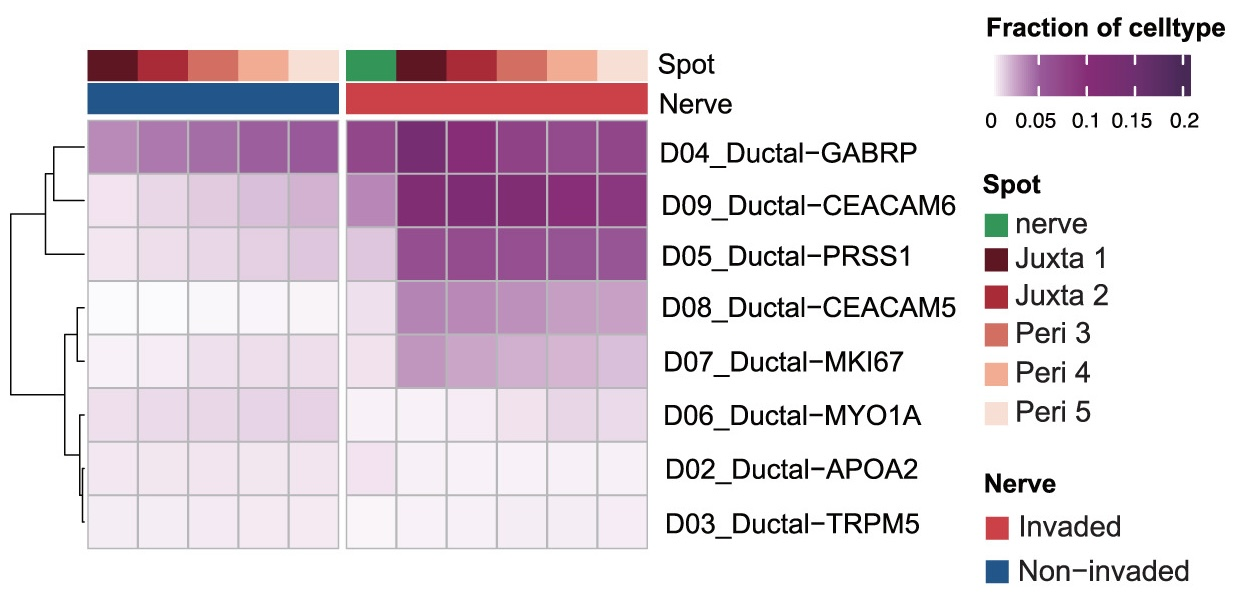
\includegraphics[width = 0.8\linewidth]{Figures/2L.jpg}
  \end{figure}
\end{frame}

\begin{frame}{Distinct invasion strategies of key malignant subtypes}
  \begin{itemize}
    \item D09\_Ductal-CEACAM6: pro-migratory and pro-invasive features
          \begin{itemize}
            \item Enriched pathways: \textbf{integrin-mediated signaling}, \textbf{ameboid-type migration}, \textbf{adhesion-dependent spreading}
            \item Exhibited the \textbf{highest EMT score} among malignant subtypes
            \item \textbf{WNT signaling} elevated, consistent with EMT activation
            \item Upregulated \textbf{CTSA} and \textbf{CTSB} (ECM-degrading proteinases)
          \end{itemize}

    \item Interpretation
          \begin{itemize}
            \item D09\_Ductal-CEACAM6 likely has \textbf{a heightened capability of migrating through the tissue matrix,}
            \item Spatial enrichment near invaded nerves suggests it may \textbf{actively drive neural invasion}
          \end{itemize}
  \end{itemize}
\end{frame}

\begin{frame}{Distinct invasion strategies of key malignant subtypes}
  \begin{itemize}
    \item D04\_Ductal-GABRP marker gene: GABRP
      \begin{itemize}
        \item GABRP encodes a receptor subunit for the inhibitory neurotransmitter \textbf{GABA}
        \item D04\_Ductal-GABRP is characterized by \textbf{high GABRP expression}
      \end{itemize}

    \item High nerve-interaction potential
      \begin{itemize}
        \item A curated NI-related, nerve-associated gene set was applied
        \item \textbf{D04\_Ductal-GABRP scored the highest} among all malignant subpopulations

              \(\Rightarrow\) Suggests \textbf{active reciprocal interactions with nerves} that may promote NI
      \end{itemize}

    \item Not dependent on GABAergic innervation
      \begin{itemize}
        \item GAD65 used as a marker for GABAergic neurons in mIHC
        \item \textbf{No GAD65\(^{+}\) neurons} detected, even in tumors rich in GABRP\(^{+}\) malignant cells
        \item Consistent with reports that \textbf{GABRP promotes tumor migration in a GABA-independent, KCNN4-synergistic manner}
      \end{itemize}

    \item GABRP-KCNN4 axis in high-NI tissues
      \begin{itemize}
        \item mIHC confirmed \textbf{co-expression of GABRP and KCNN4} in malignant cells in high-NI tissues
      \end{itemize}
  \end{itemize}
\end{frame}

\begin{frame}{Distinct invasion strategies of key malignant subtypes}
  \begin{columns}[T,onlytextwidth]
    \begin{column}{0.5\textwidth}
      \begin{figure}
        \centering
        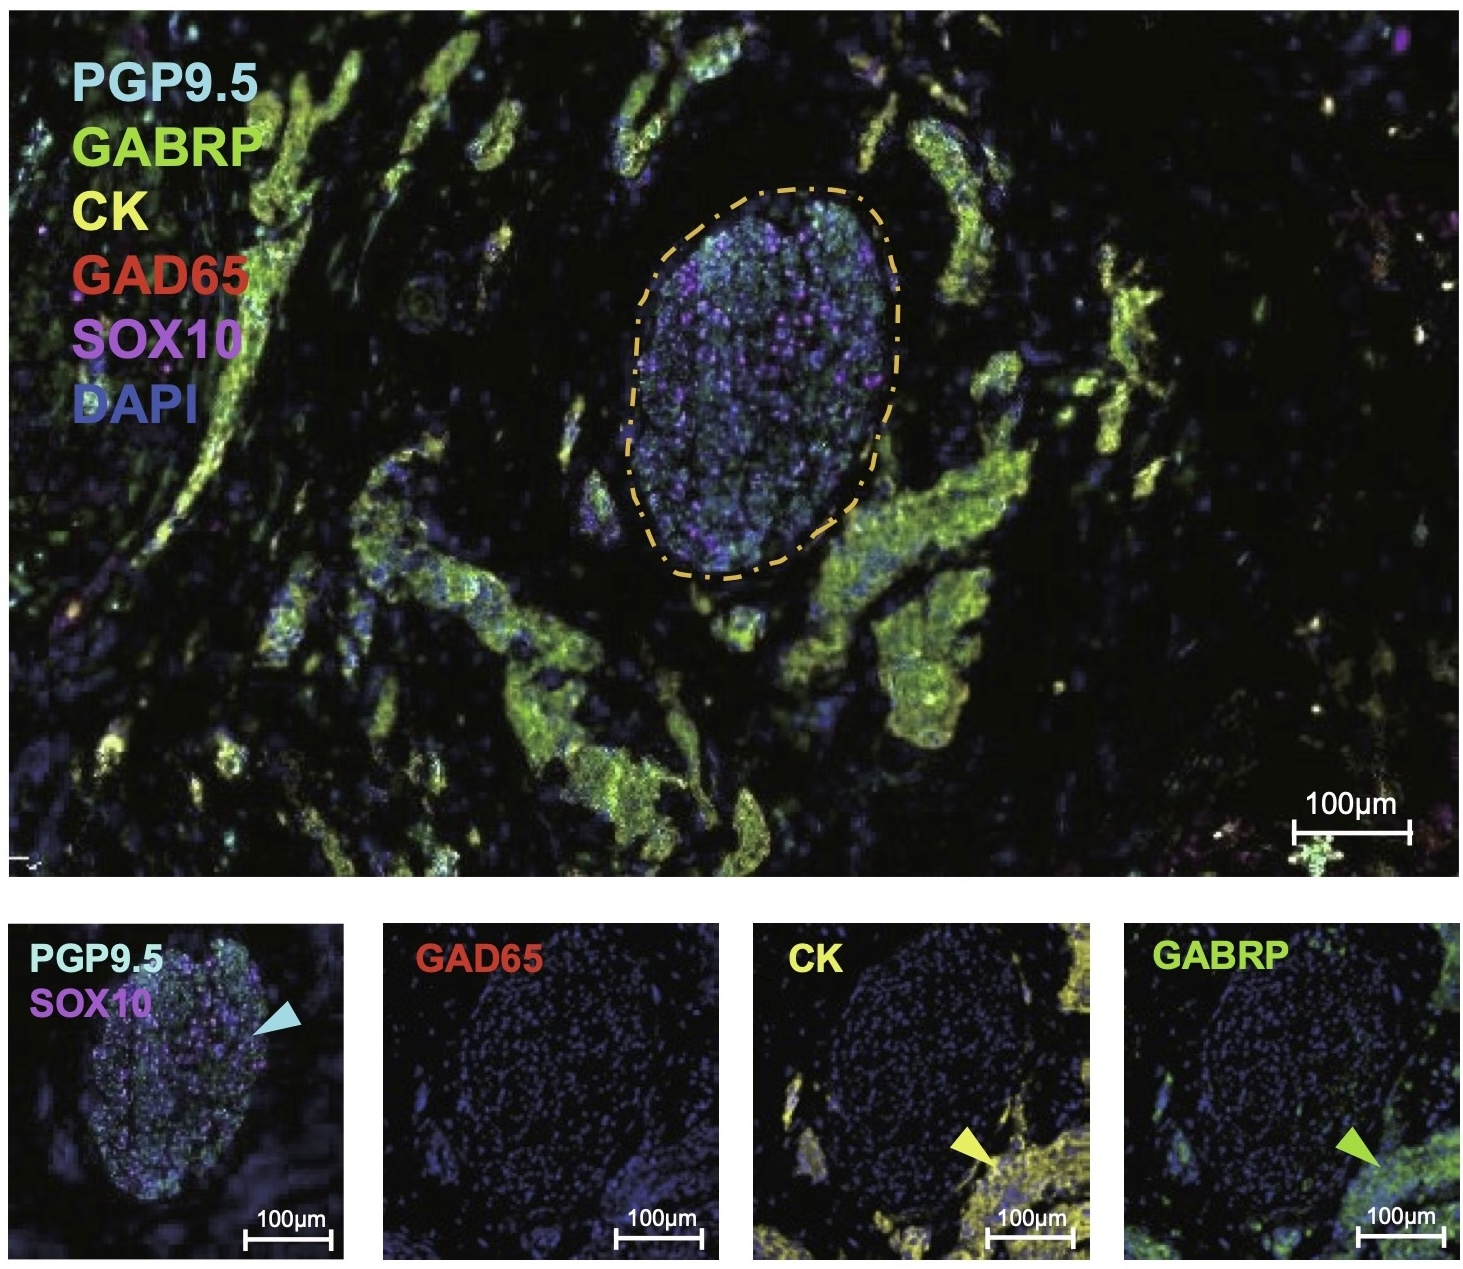
\includegraphics[width = 0.9\linewidth]{Figures/S3K.jpg}
      \end{figure}
      \begin{itemize}
        \item mIHC staining showing absence of GAD65+ GABAergic neurons in PDAC tissues with high proportion of GABRP+ malignant cells
      \end{itemize}
    \end{column}
    \begin{column}{0.5\textwidth}
      \begin{figure}
        \centering
        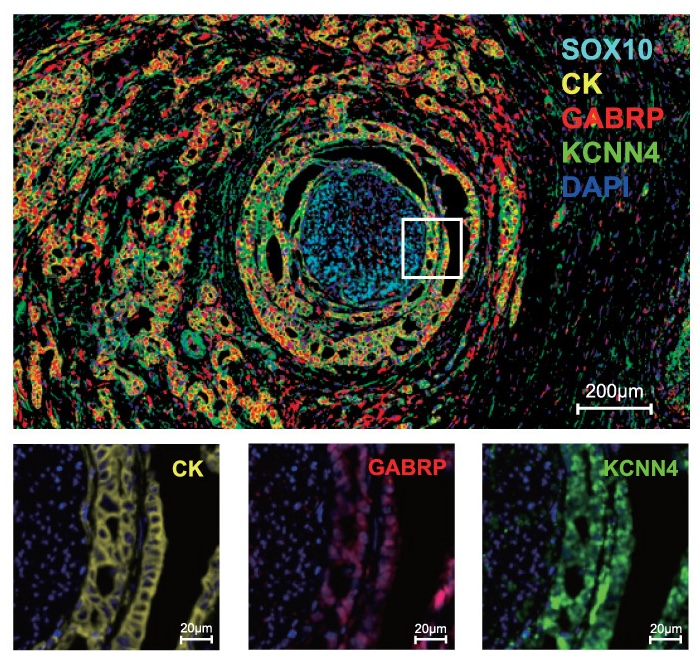
\includegraphics[width = 0.9\linewidth]{Figures/2N.jpg}
      \end{figure}
      \begin{itemize}
        \item mIHC staining showing co-expression of GABRP and KCNN4 in malignant cells
      \end{itemize}
    \end{column}
  \end{columns}
\end{frame}

\begin{frame}{Part 1 Summary: Malignant ductal subpopulations \& NI}
  \begin{itemize}
    \item \textbf{Ductal atlas}
      \begin{itemize}
        \item 9 ductal subclusters (D01--D09) identified by sc/snRNA-seq.
        \item D01\_Ductal-CFTR: low CNV, transcriptionally normal ductal cells.
        \item D02--D09: malignant ductal states spanning \textbf{classical}, \textbf{basal-like}, intermediate and \textbf{neuroendocrine-like} programs.
      \end{itemize}
    \item \textbf{Low-NI tumors}
      \begin{itemize}
        \item Enriched for D02\_Ductal-APOA2 (neuroendocrine-like, Malignant\_ductal\_4 niche).
        \item High lipid/cholesterol metabolism, low NI-related gene scores and low EMT score
              \(\Rightarrow\) \textbf{less invasive phenotype}.
      \end{itemize}
    \item \textbf{High-NI tumors}
      \begin{itemize}
        \item Reduced malignant subtype diversity; dominated by basal-like, intermediate and classical states.
        \item D09\_Ductal-CEACAM6 (basal-like): strong EMT, integrin-mediated migration, WNT signaling and ECM proteases
              \(\Rightarrow\) \textbf{high intrinsic migratory/invasive capacity}.
        \item D04\_Ductal-GABRP (intermediate): highest NI-related gene-set scores and enriched near invaded nerves;
              GABRP-KCNN4 axis supports tumor migration in a \textbf{GABA-independent} manner.
      \end{itemize}
  \end{itemize}
\end{frame}

%==================== Part 2 ====================%
\subsection{Part 2: Tumor microenvironment and neural invasion}

\begin{frame}{Part 2 Overview}
  \begin{itemize}
    \item Question: How do immune \& stromal compartments differ between low- and high-NI PDAC?
    \item Strategy:
      \begin{itemize}
        \item Integrate sc/snRNA-seq and ST from 21 PDAC patients (5 low-NI, 16 high-NI).
        \item Quantify enrichment using ratio of observed to expected cell numbers (Ro/e), miloR and spatial deconvolution.
        \item Zoom into juxta-neural regions of invaded vs non-invaded nerves.
      \end{itemize}
    \item Key message:
      \begin{itemize}
        \item Low-NI tumors are enriched for TLS-centered immunity, whereas high-NI tumors show inflammatory and immunosuppressive microenvironments around nerves.
      \end{itemize}
  \end{itemize}
\end{frame}

\begin{frame}{Low-NI TME: TLS-centered anti-tumor immunity}
  \begin{itemize}
    \item \textbf{B cell / plasma cell} enrichment in low-NI tumors
      \begin{itemize}
        \item Increased ratios of:
          \begin{itemize}
            \item B03\_GCB-RGS13 (germinal center B cells)
            \item B06\_plasmablasts-MKI67
            \item B05\_PlasmaB-IgG
          \end{itemize}
      \end{itemize}
      \(\Rightarrow\) Indicates more active \textbf{germinal center and plasma cell responses} in low-NI tissues
  \end{itemize}
  \begin{figure}
    \centering
    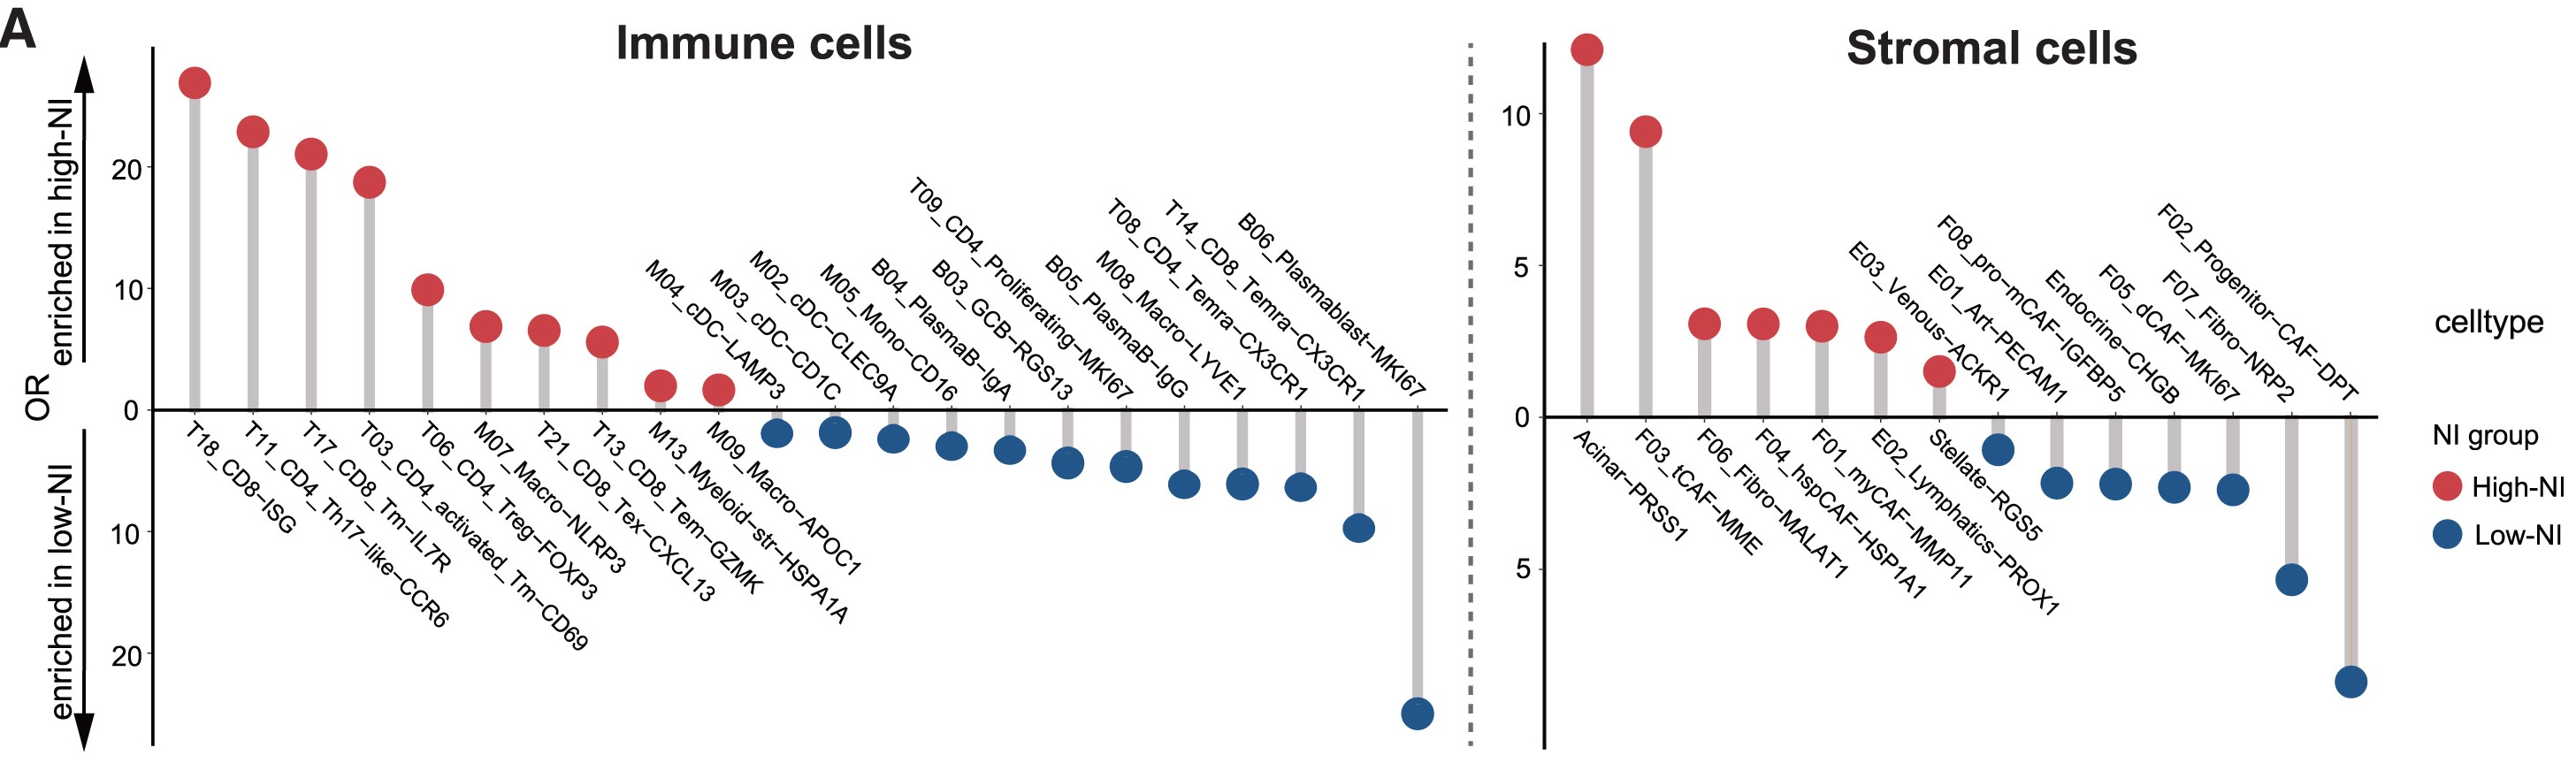
\includegraphics[width = \linewidth]{Figures/3A.jpg}
  \end{figure}
\end{frame}


\begin{frame}{Low-NI TME: TLS-centered anti-tumor immunity}
  \begin{itemize}
    \item Evidence for \textbf{increased TLS abundance in low-NI}
      \begin{itemize}
        \item GCBs primarily reside in \textbf{TLSs} and differentiate into plasma cells within TLSs
        \item ST showed higher proportions of key TLS components in low-NI tissues:
          \begin{itemize}
            \item B01\_naive-TCL1A
            \item B03\_GCB-RGS13
            \item T10\_CD4\_Tfh-like CXCL13
          \end{itemize}
      \end{itemize}

    \item \textbf{TLS-/B cell-related spatial niches in low-NI}
      \begin{itemize}
        \item PCA of spatial niches revealed a \textbf{distinct cluster} for low-NI tissues
        \item Low-NI group showed higher proportions of:
          \begin{itemize}
            \item \textbf{N01\_TLS niche}
            \item N04\_Plasma-enriched niche
            \item N03\_Perivascular niche
          \end{itemize}
      \end{itemize}
      \(\Rightarrow\) Organized \textbf{TLS-like structures} and \textbf{B cell immunity} are associated with the \textbf{low-NI status} in PDAC
  \end{itemize}
\end{frame}

\begin{frame}{CD8 T cell dynamics and TLS in low-NI vs high-NI PDAC}
  \begin{itemize}
    \item \textbf{Effector CD8\_Temra} enrichment in low-NI tumors
      \begin{itemize}
        \item \textbf{T14\_CD8\_Temra CX3CR1}: effector memory CD8 subset with high cytotoxic gene expression
        \item Exhibited \textbf{higher infiltration} in low-NI tumor tissues
      \end{itemize}
  \end{itemize}
  \begin{figure}
    \centering
    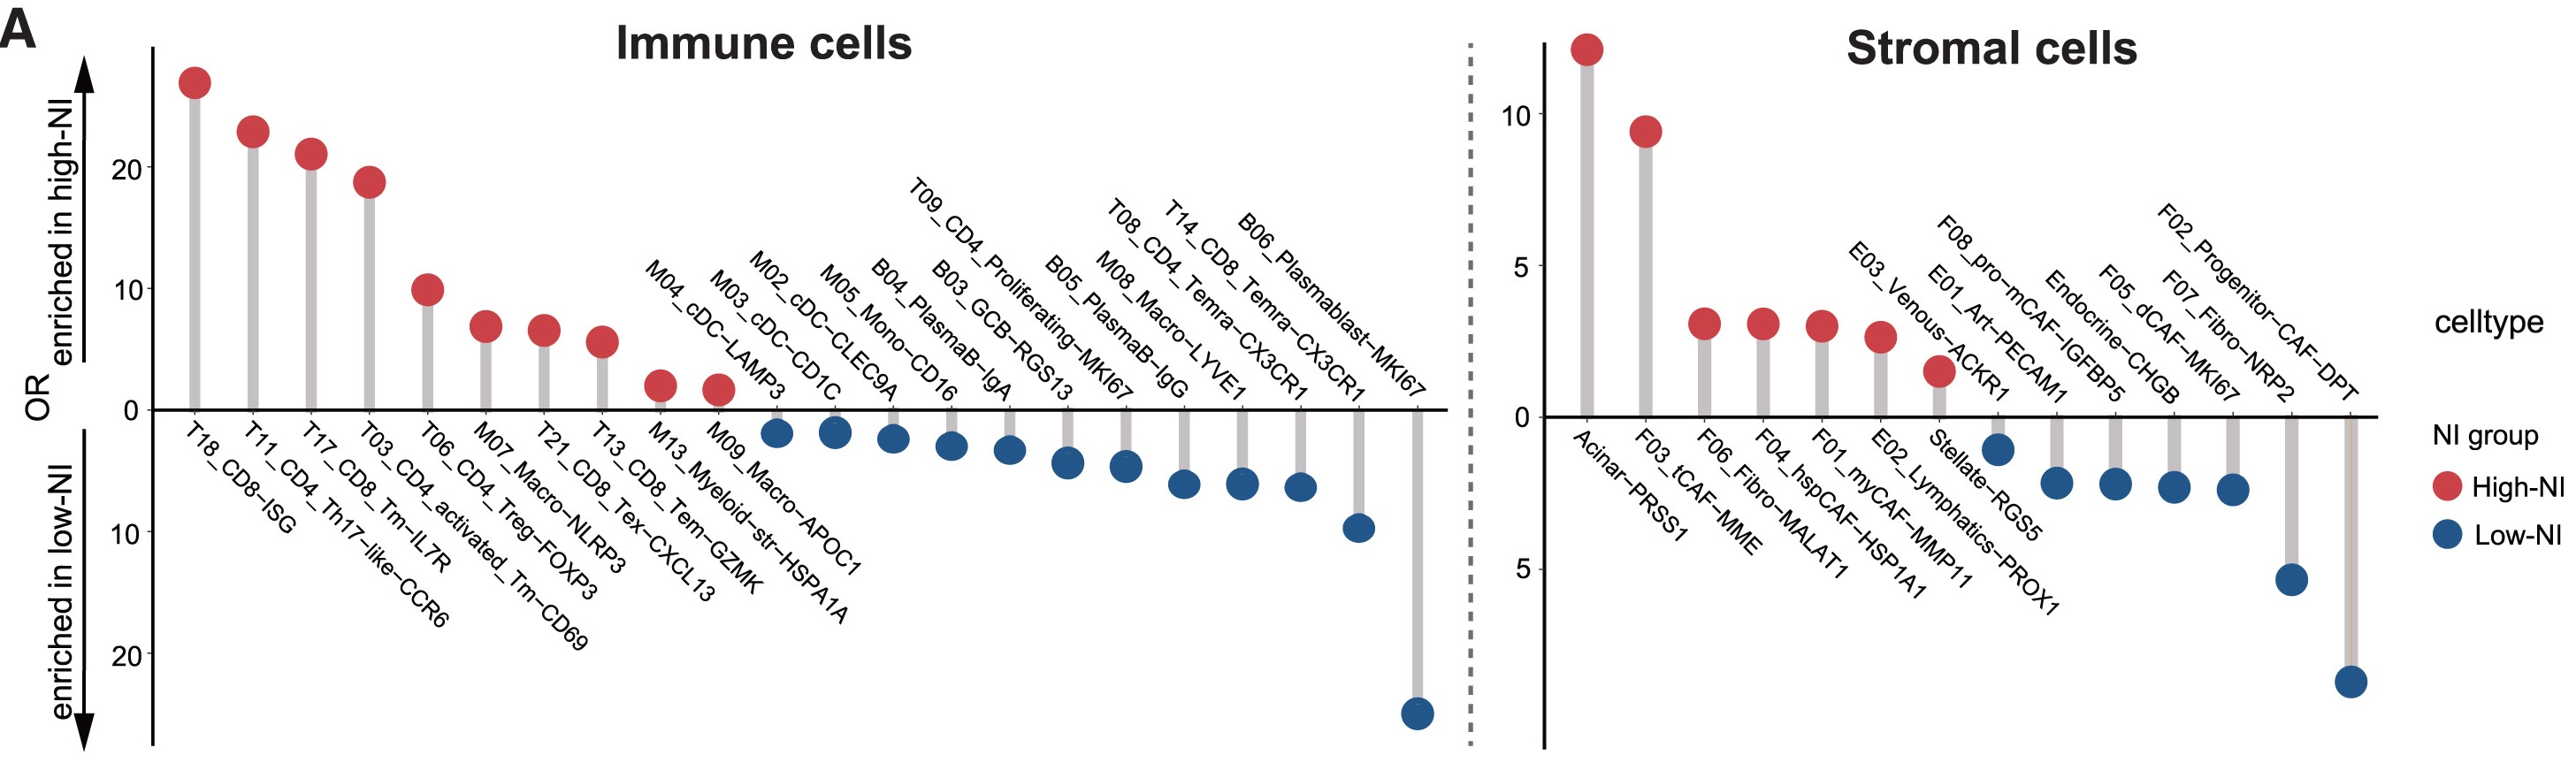
\includegraphics[width = \linewidth]{Figures/3A.jpg}
  \end{figure}
\end{frame}

\begin{frame}{CD8 T cell dynamics and TLS in low-NI vs high-NI PDAC}
  \begin{itemize}

    \item Clonal expansion and migration of CD8\_Temra in low-NI
      \begin{itemize}
        \item scTCR-seq + STARTRAC used to trace T cell clonal dynamics
        \item In low-NI group:
          \begin{itemize}
            \item CD8\_Temra showed \textbf{robust clonal expansion} in tumors
            \item Displayed the \textbf{highest migration from blood} among T cell subsets
          \end{itemize}
        \(\Rightarrow\) Origin from both \textbf{in situ expansion} and \textbf{peripheral blood recruitment}
      \end{itemize}

    \item Spatial localization: TLS-/plasma-/vascular niches
      \begin{itemize}
        \item ST localized CD8\_Temra mainly to \textbf{N01, N04 and N03 niche}.
        \item Consistent with \textbf{expansion within TLS-like structures} and \textbf{migration from vasculature}
      \end{itemize}
    \item Histology: CD8\_Temra observed at the \textbf{periphery of TLS-like structures}, mirroring plasma cell distribution
  \end{itemize}
  \begin{figure}
    \centering
    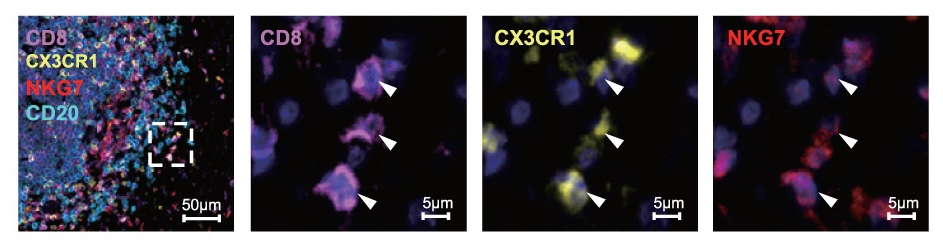
\includegraphics[width = 0.8\linewidth]{Figures/3G.jpg}
  \end{figure}
\end{frame}

\begin{frame}{CD8 T cell dynamics and TLS in low-NI vs high-NI PDAC}
  \begin{itemize}
    \item High-NI: \textbf{weakened effector CD8 response, more exhaustion}
      \begin{itemize}
        \item In high-NI group, CD8\_Temra showed \textbf{reduced expansion and migration} and lower representation in N01\_TLS niche
        \item \textbf{Tex (exhausted CD8 T cells)} were more abundant in high-NI tissues
        \item Tex preferentially localized to \textbf{ductal-enriched niches}, not TLS-related regions
      \end{itemize}
    \(\Rightarrow\) TLSs may generate effector CD8 T cells counteracting invasion in low-NI, whereas high-NI tumors exhibit \textbf{exhausted, TLS-independent CD8 immunity}
  \end{itemize}
  \begin{columns}[T,onlytextwidth]
    \begin{column}{0.45\textwidth}
      \begin{figure}
        \centering
        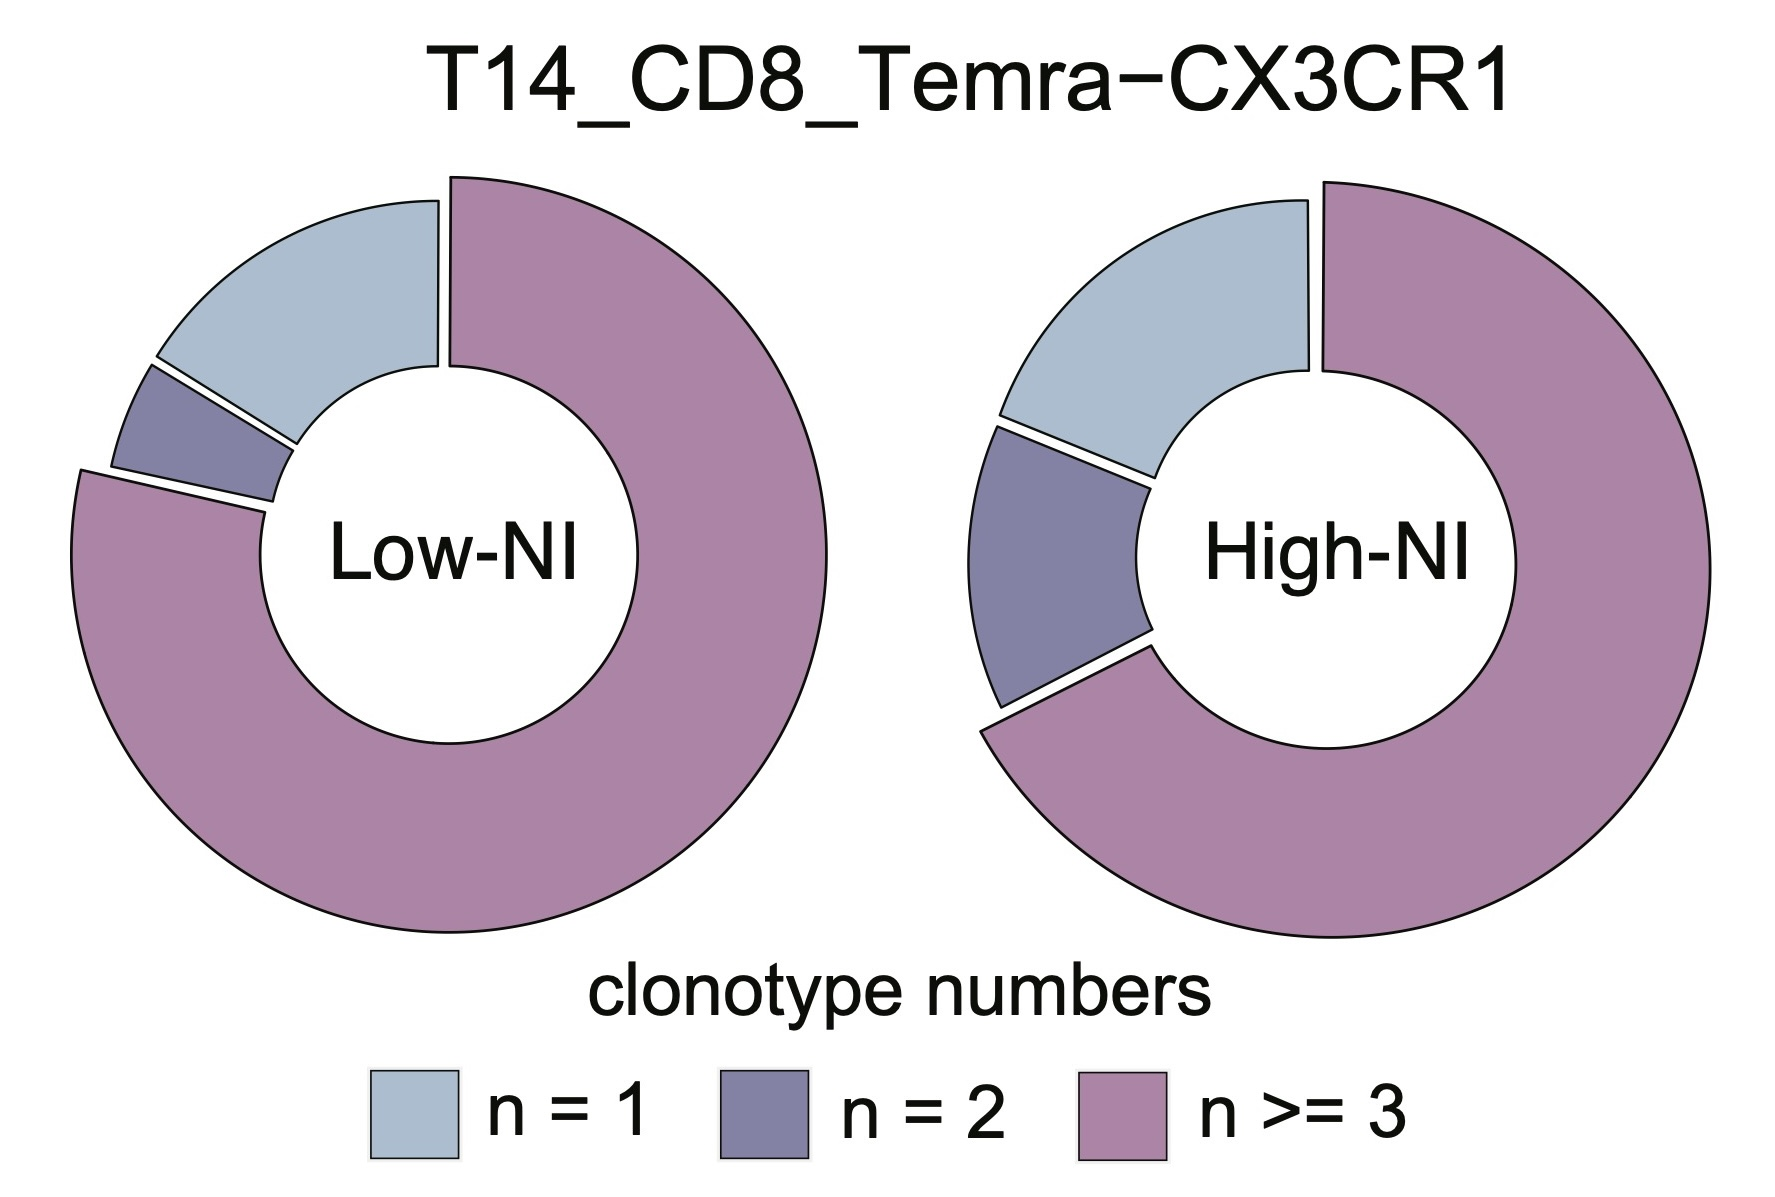
\includegraphics[width = 0.9\linewidth]{Figures/S4E.jpg}
      \end{figure}
    \end{column}
    \begin{column}{0.55\textwidth}
      \begin{figure}
        \centering
        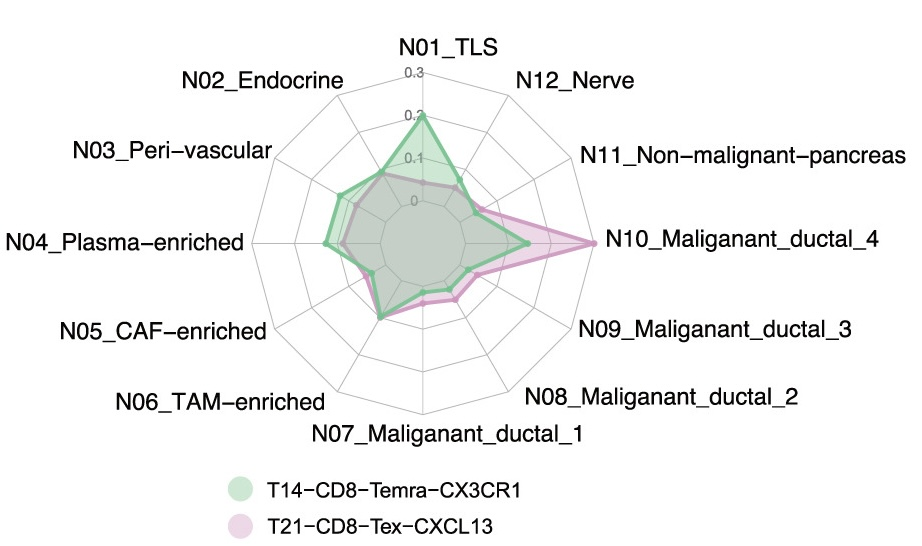
\includegraphics[width = 0.9\linewidth]{Figures/3F.jpg}
      \end{figure}
    \end{column}
  \end{columns}
\end{frame}

\begin{frame}{High-NI TME: inflammatory and immunosuppressive}
  \begin{itemize}
    \item \textbf{Regulatory T cells}:
      \begin{itemize}
        \item T06\_CD4\_Treg-FOXP3 proportion increased in high-NI tumors.
        \item Likely contributes to \textbf{suppression of anti-tumor immunity}.
      \end{itemize}
    \item \textbf{Pro-inflammatory macrophages}:
      \begin{itemize}
        \item M07\_Macro-NLRP3 enriched in high-NI tissues.
        \item High IL1B expression and pathways related to \textbf{inflammatory response}.
      \end{itemize}
    \item Th17-like CD4\(^{+}\) T cells:
      \begin{itemize}
        \item Co-occurrence of M07\_Macro-NLRP3 with T11\_CD4\_Th17-like-CCR6, suggesting TAM-driven Th17 polarization.
      \end{itemize}
    \item Implication: high-NI TME combines \textbf{chronic inflammation with immunosuppression}, promoting tumors.
  \end{itemize}
\end{frame}

\begin{frame}{Stromal CAF subtypes reprogramming in high-NI tumors}
  \begin{columns}[T,onlytextwidth]
    \begin{column}{0.55\textwidth}
      \begin{itemize}
        \item \textbf{myCAF and tCAF expansion}:
          \begin{itemize}
            \item F01\_myCAF-MMP11 and F03\_tCAF-MME increased in high-NI tissues.
            \item Express \textbf{ECM remodeling, hypoxia and angiogenesis-related genes}.
          \end{itemize}
        \item Loss of \textbf{progenitor-like CAFs}:
          \begin{itemize}
          \item F02\_Progenitor-CAF-DPT (PI16\(^{+}\) progenitor-like CAFs) relatively enriched in low-NI tissues.
          \end{itemize}
        \item ST validation:
          \begin{itemize}
            \item External ST cohort confirms myCAF enrichment in high-NI and progenitor-CAF predominance in low-NI.
          \end{itemize}
      \end{itemize}
    \end{column}
    \begin{column}{0.45\textwidth}
      \begin{figure}
        \centering
        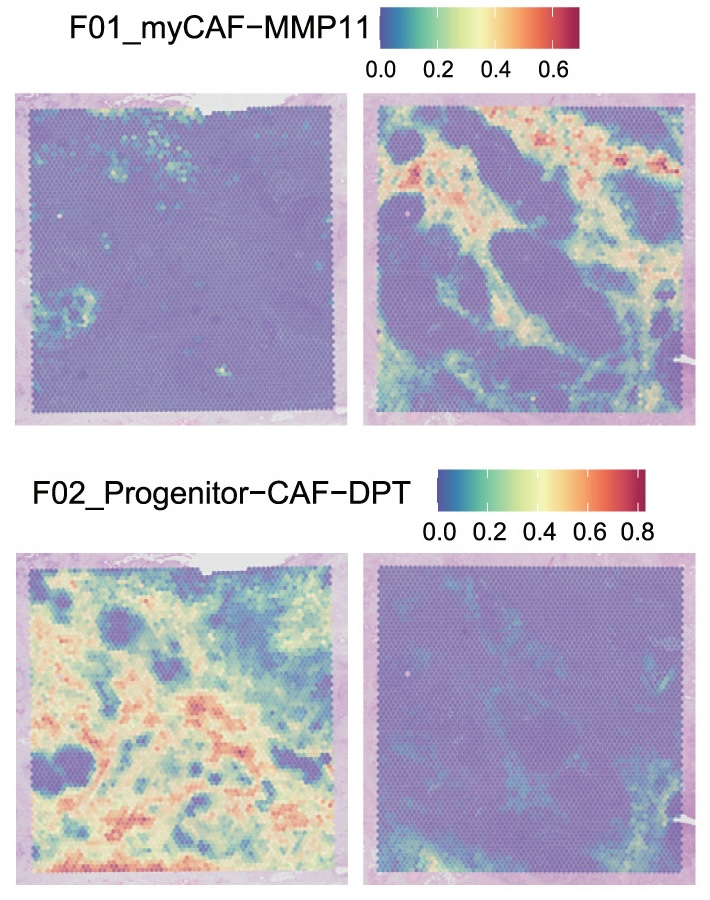
\includegraphics[width = 0.8\linewidth]{Figures/3J.jpg}
      \end{figure}
      \begin{itemize}
        \item Low NI (left), high NI (right)
      \end{itemize}
    \end{column}
  \end{columns}
  \begin{itemize}
    \item Implication: \textbf{stromal remodeling in high-NI tumors may facilitate nerve invasion and tumor spread.}
  \end{itemize}
\end{frame}

\begin{frame}{Part 2 Summary: TME states linked to NI status}
  \begin{itemize}
    \item \textbf{Low-NI tumors: TLS-centered, effector-dominant immunity}
      \begin{itemize}
        \item Enriched in \textbf{germinal center B cells}, plasmablasts and plasma cells.
        \item Higher abundance of \textbf{TLS components} and TLS-/plasma-/perivascular niches (N01, N04, N03).
        \item Clonally expanded, cytotoxic \textbf{CD8\_Temra CX3CR1} cells localize to TLS/perivascular regions.
      \end{itemize}

    \item \textbf{High-NI tumors: inflammatory and immunosuppressive niches}
      \begin{itemize}
        \item More \textbf{exhausted CD8 Tex} in ductal-enriched niches; reduced CD8\_Temra expansion and migration.
        \item Increased \textbf{Tregs}, \textbf{NLRP3\(^{+}\) macrophages} and Th17-like CD4\(^{+}\) T cells.
        \item Expansion of \textbf{myCAF/tCAF} and loss of progenitor-like CAFs; myCAF/tCAF accumulate around invaded nerves.
      \end{itemize}
    \item \textbf{Conceptual model}
      \begin{itemize}
        \item \textbf{Low-NI: ``protective'' TLS-rich, B/Temra-supported microenvironments around nerves.}
        \item \textbf{High-NI: ``pro-invasive'' niches dominated by inflammation, immunosuppression and CAF-driven remodeling.}
      \end{itemize}
  \end{itemize}
\end{frame}

%==================== Part 3 ====================%
\subsection{Part 3: Juxta-neural microenvironment and nerve-resident cells}

\begin{frame}{Part 3 Overview}
  \begin{columns}[T,onlytextwidth]
    \begin{column}{0.6\textwidth}
      \begin{itemize}
        \item Question:
          \begin{itemize}
            \item How do the cellular and molecular landscapes differ around \textbf{non-invaded} vs \textbf{invaded} nerves?
          \end{itemize}
      \end{itemize}
    \end{column}
    \begin{column}{0.4\textwidth}
      \begin{figure}
        \centering
        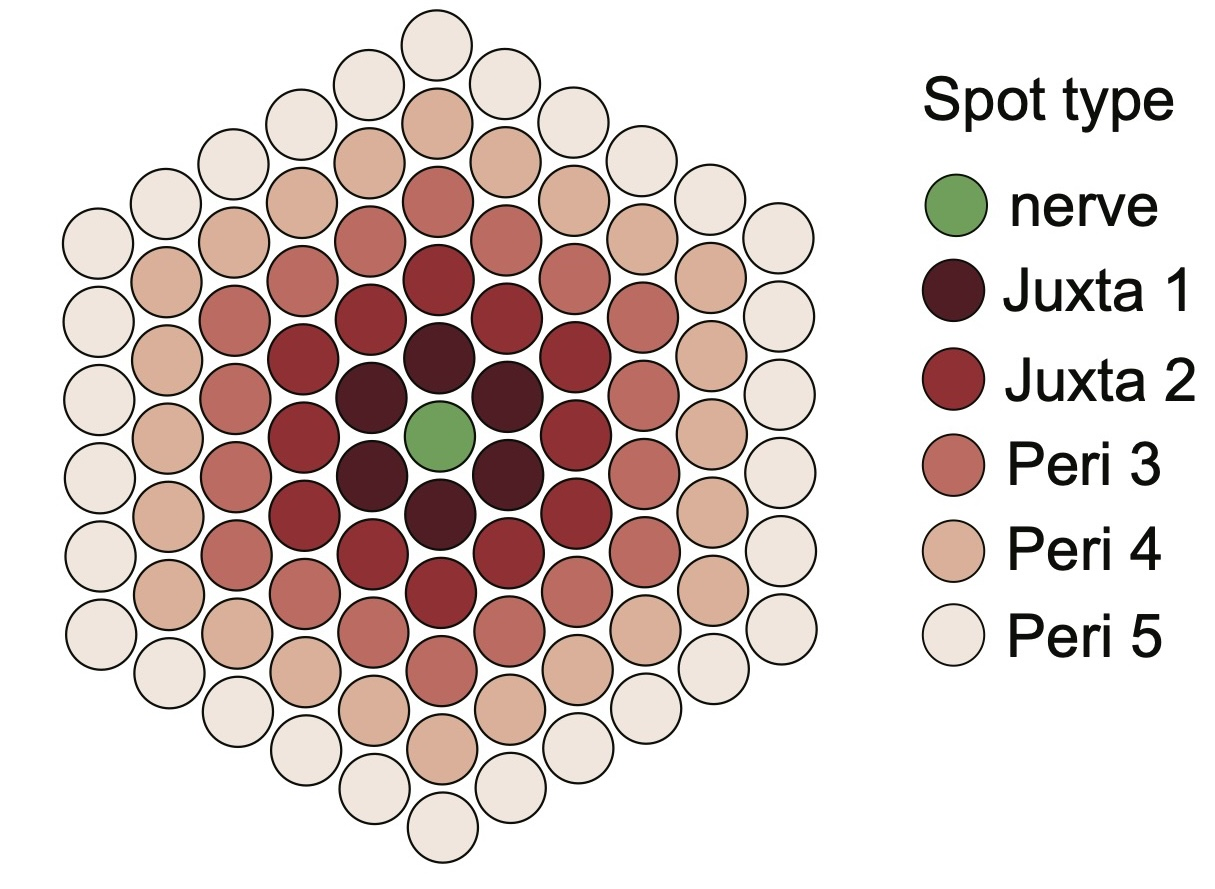
\includegraphics[width = 0.6\linewidth]{Figures/S5A.jpg}
      \end{figure}
    \end{column}
  \end{columns}
  \vspace{-0.55cm}
  \begin{itemize}
    \item Strategy:
      \begin{itemize}
        \item Define ``nerve spots'' (overlapping with nerves) and juxta-neural rings (two layers, \(\sim 200\,\upmu\text{m}\)) around nerves in ST data.
        \item Compare cell-type composition, spatial niches and signaling pathways between non-invaded and invaded nerves.
        \item Integrate sc/snRNA-seq, ST, COMMOT communication analysis, MISTy spatial modelling and mIHC.
      \end{itemize}
    \item Key message:
      \begin{itemize}
        \item \textbf{Non-invaded nerves} are embedded in \textbf{TLS-rich, adaptive immune} microenvironments.
        \item \textbf{Invaded nerves} are surrounded by \textbf{innate inflammatory} and \textbf{T cell-exhausted} niches with stromal remodeling.
      \end{itemize}
  \end{itemize}
\end{frame}

\begin{frame}{Nerve-TLS structures (NTSs) around non-invaded nerves}
  \begin{itemize}
    \item \textbf{Cellular composition} around non-invaded nerves
      \begin{itemize}
        \item Juxta-neural regions enriched for \textbf{TLS components}: B03\_GCB-RGS13 (germinal center B cells), T10\_CD4\_Tfh-like CXCL13, M04\_cDC-LAMP3.
        \item Fractions of N01\_TLS and N04\_Plasma-enriched niches \textbf{increase} as distance to non-invaded nerves declines.
        \item This spatial gradient is \textbf{not} observed around invaded nerves.
      \end{itemize}
    \item \textbf{Nerve-TLS association}
      \begin{itemize}
        \item Among 141 non-invaded nerve fibers in tumors, \(\sim 64\%\) had a TLS within \(100\,\upmu\text{m}\) of the nerve border.
        \item Non-invaded nerves in adjacent normal tissues were \textbf{less} associated with TLSs
              \(\Rightarrow\) TLS formation around nerves is \textbf{tumor-associated}.
        \item Among all tumor TLSs, \(\sim 50\%\) had a nerve fiber within \(100\,\upmu\text{m}\)
              \(\Rightarrow\) \textbf{nerve-TLS structures (NTSs)} are common in PDAC.
      \end{itemize}
  \end{itemize}
  \begin{figure}
    \centering
    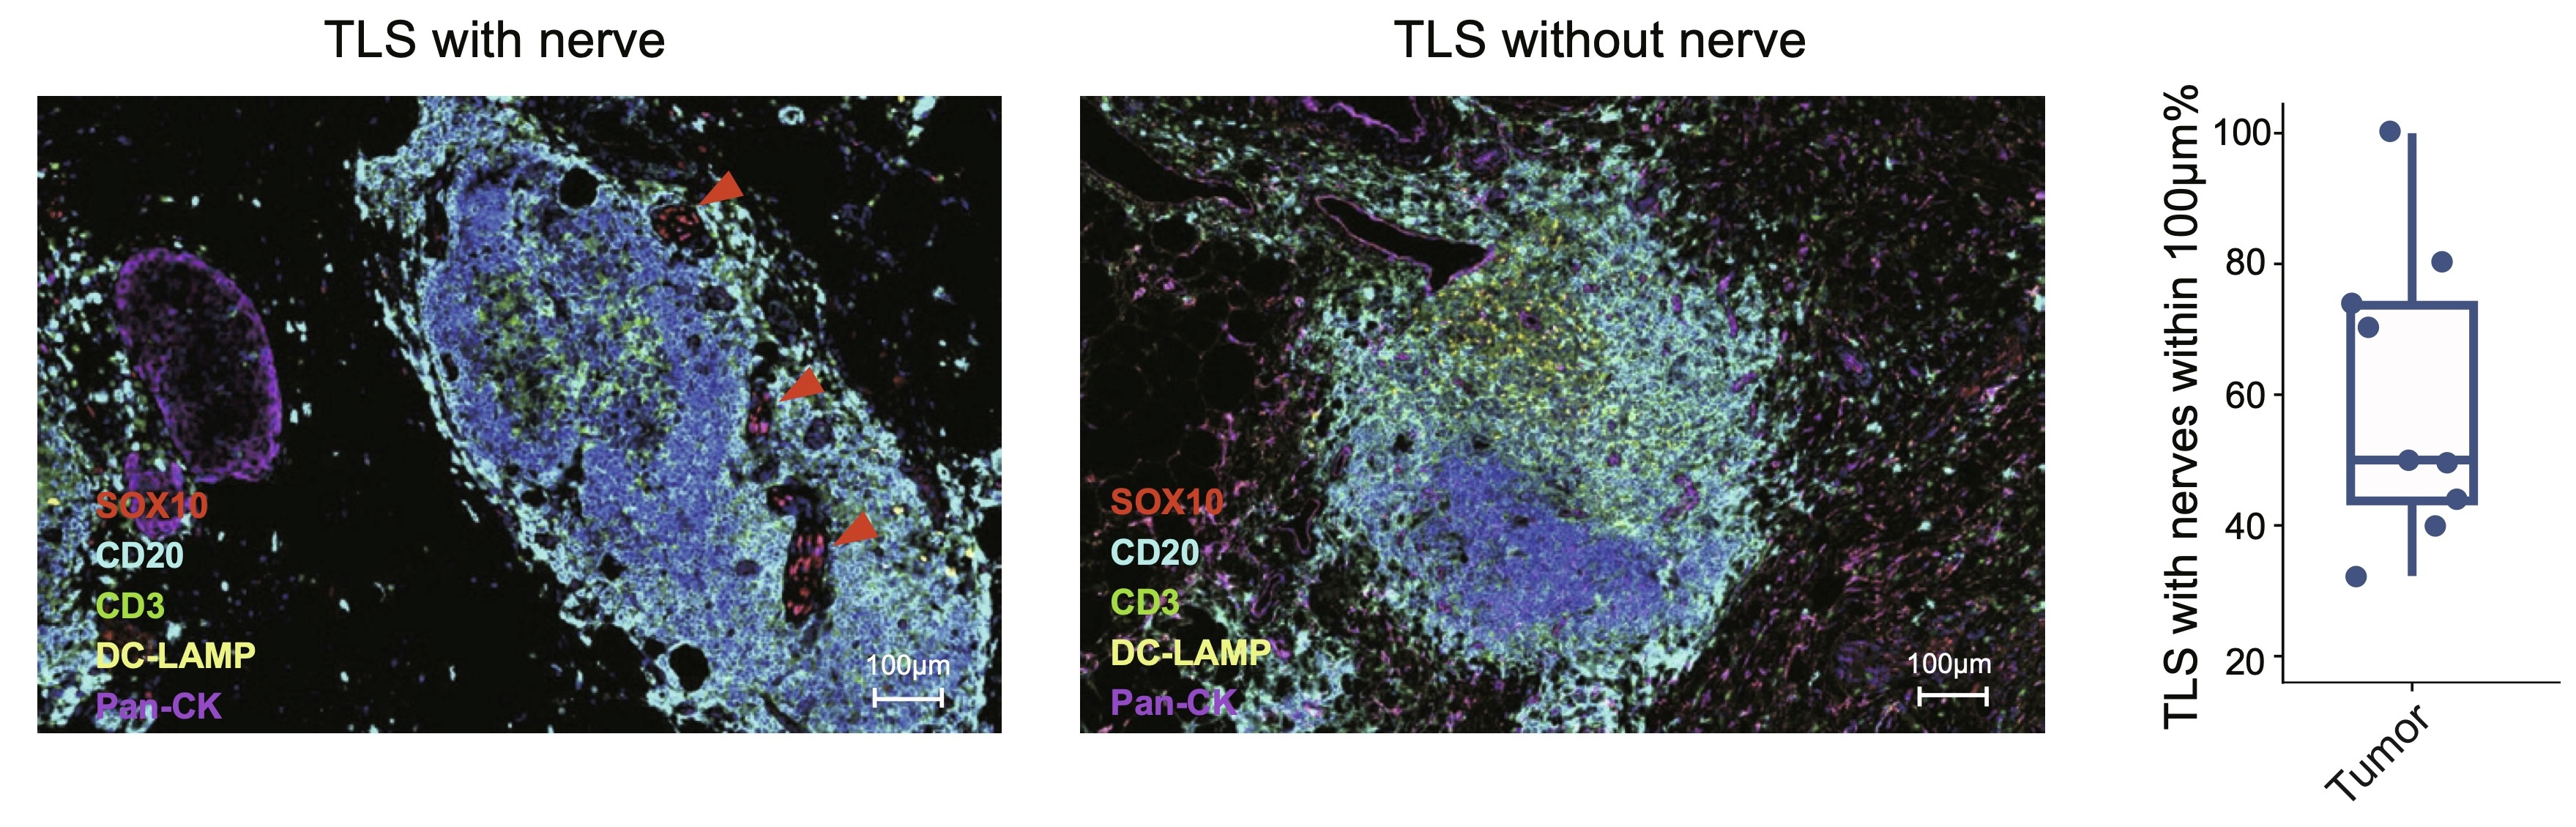
\includegraphics[width = 0.8\linewidth]{Figures/S5E.jpg}
  \end{figure}  
\end{frame}

\begin{frame}{Signaling environment around non-invaded vs invaded nerves}
  \begin{columns}[T,onlytextwidth]
    \begin{column}{0.6\textwidth}
      \begin{itemize}
        \item \textbf{COMMOT analysis} of juxta-neural neighborhoods
          \begin{itemize}
            \item Optimal-transport-based inference of spatial ligand-receptor signaling between cell populations
            \item Modelled secreted signaling, cell-cell contact and ECM-receptor pathways using ligand-receptor expression
          \end{itemize}
        \item Non-invaded nerves: \textbf{adaptive immune-supportive signals}
          \begin{itemize}
            \item Elevated pathways for \textbf{leukocyte recruitment}: CXCL, CCL, IL-16.
            \item Elevated pathways for \textbf{lymphocyte proliferation and differentiation}: BAFF, APRIL, IL-2, LIGHT, CD40.
            \item Indicates an \textbf{active signaling environment} supporting TLS construction and adaptive immune responses.
          \end{itemize}
      \end{itemize}
    \end{column}
    \begin{column}{0.4\textwidth}
      \begin{figure}
        \centering
        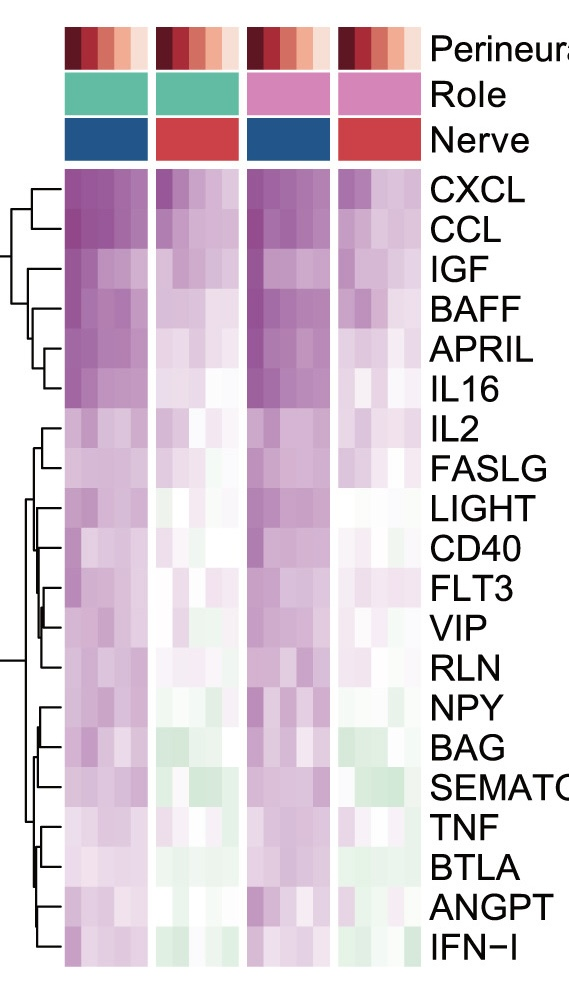
\includegraphics[width=0.9\linewidth]{Figures/4F.jpg}
      \end{figure}
    \end{column}
  \end{columns}
\end{frame}

\begin{frame}{Signaling environment around non-invaded vs invaded nerves}
  \begin{figure}
    \centering
    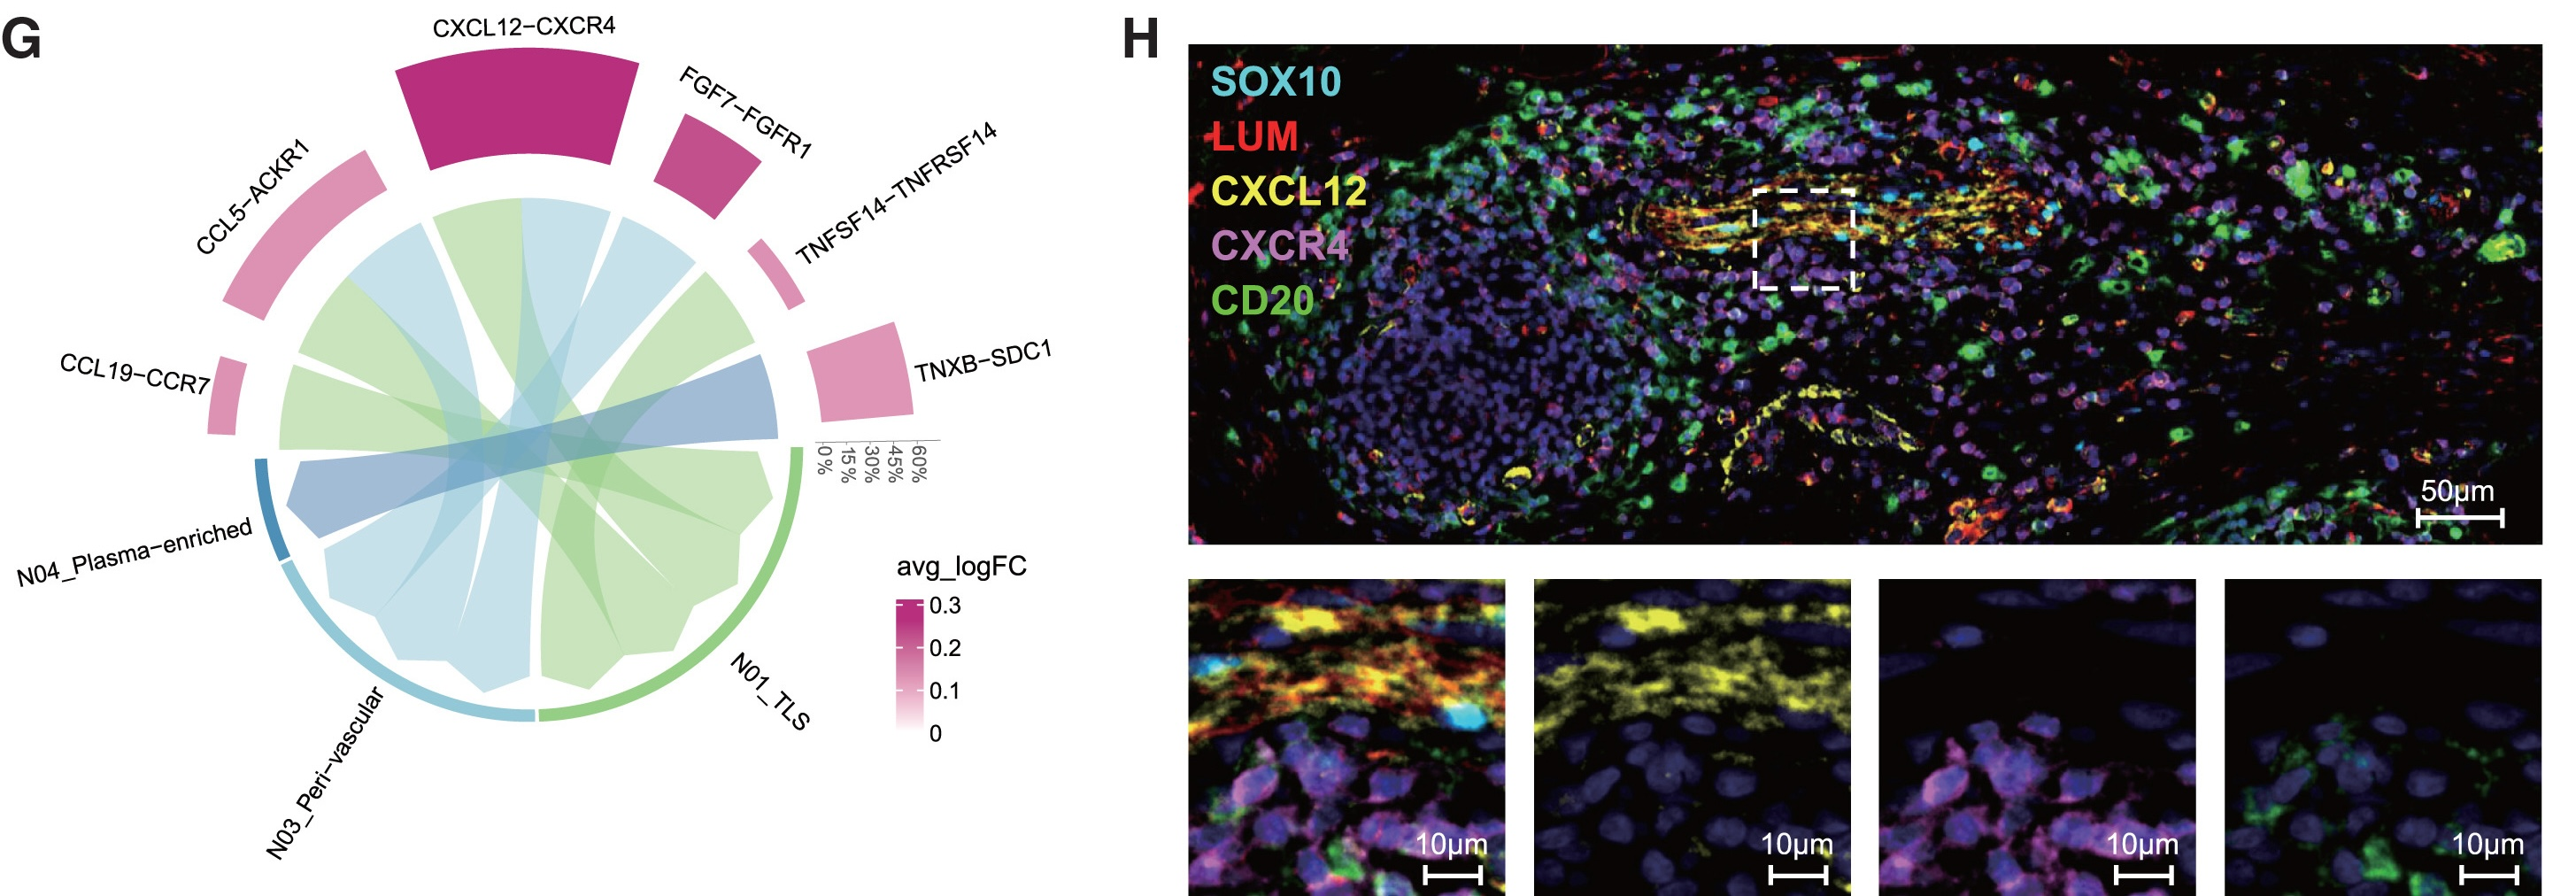
\includegraphics[width = 0.9\linewidth]{Figures/4G&H.jpg}
  \end{figure}
  \begin{itemize}
    \item \textbf{CXCL12-CXCR4 axis and TLS organization}
      \begin{itemize}
        \item Comparing non-invaded vs invaded nerve spots highlighted candidate ligand-receptor pairs.
        \item mIHC showed abundant CXCL12 in fibroblasts inside and around nerves.
        \item Suggests that \textbf{nerve-associated fibroblasts} may secrete CXCL12 to recruit CXCR4\(^{+}\) B cells and facilitate TLS assembly.
        \item Aligns with previous reports implicating stromal- and epithelial-derived CXCL12 in TLS induction.
      \end{itemize}
  \end{itemize}
\end{frame}

\begin{frame}{Invaded nerves: inflammatory and immunosuppressive niches}
  \begin{itemize}
    \item Immunosuppressive pathways around invaded nerves
      \begin{itemize}
        \item Increased \textbf{IL-10 and TGF-\(\upbeta\) signaling} in juxta-neural regions.
        \item Higher expression of \textbf{T cell exhaustion markers} than around non-invaded nerves.
      \end{itemize}
    \item \textbf{Pro-inflammatory IL-1 signaling}
      \begin{itemize}
        \item Upregulated IL-1 pathway around invaded nerves.
        \item M07\_Macro-NLRP3, enriched near invaded nerves, expresses high IL1B, reminiscent of \textbf{wound-like} inflammatory responses.
      \end{itemize}
    \item Conceptual contrast
      \begin{itemize}
        \item \textbf{Non-invaded nerves:} TLS construction and adaptive immune protective environment.
        \item \textbf{Invaded nerves:} innate inflammatory niche (inflammatory macrophages and neutrophils) combined with \textbf{T cell exhaustion} and immunosuppression.
      \end{itemize}
  \end{itemize}
\end{frame}

\begin{frame}{Cellular composition of non-invaded and invaded nerves}
  \begin{figure}
    \centering
    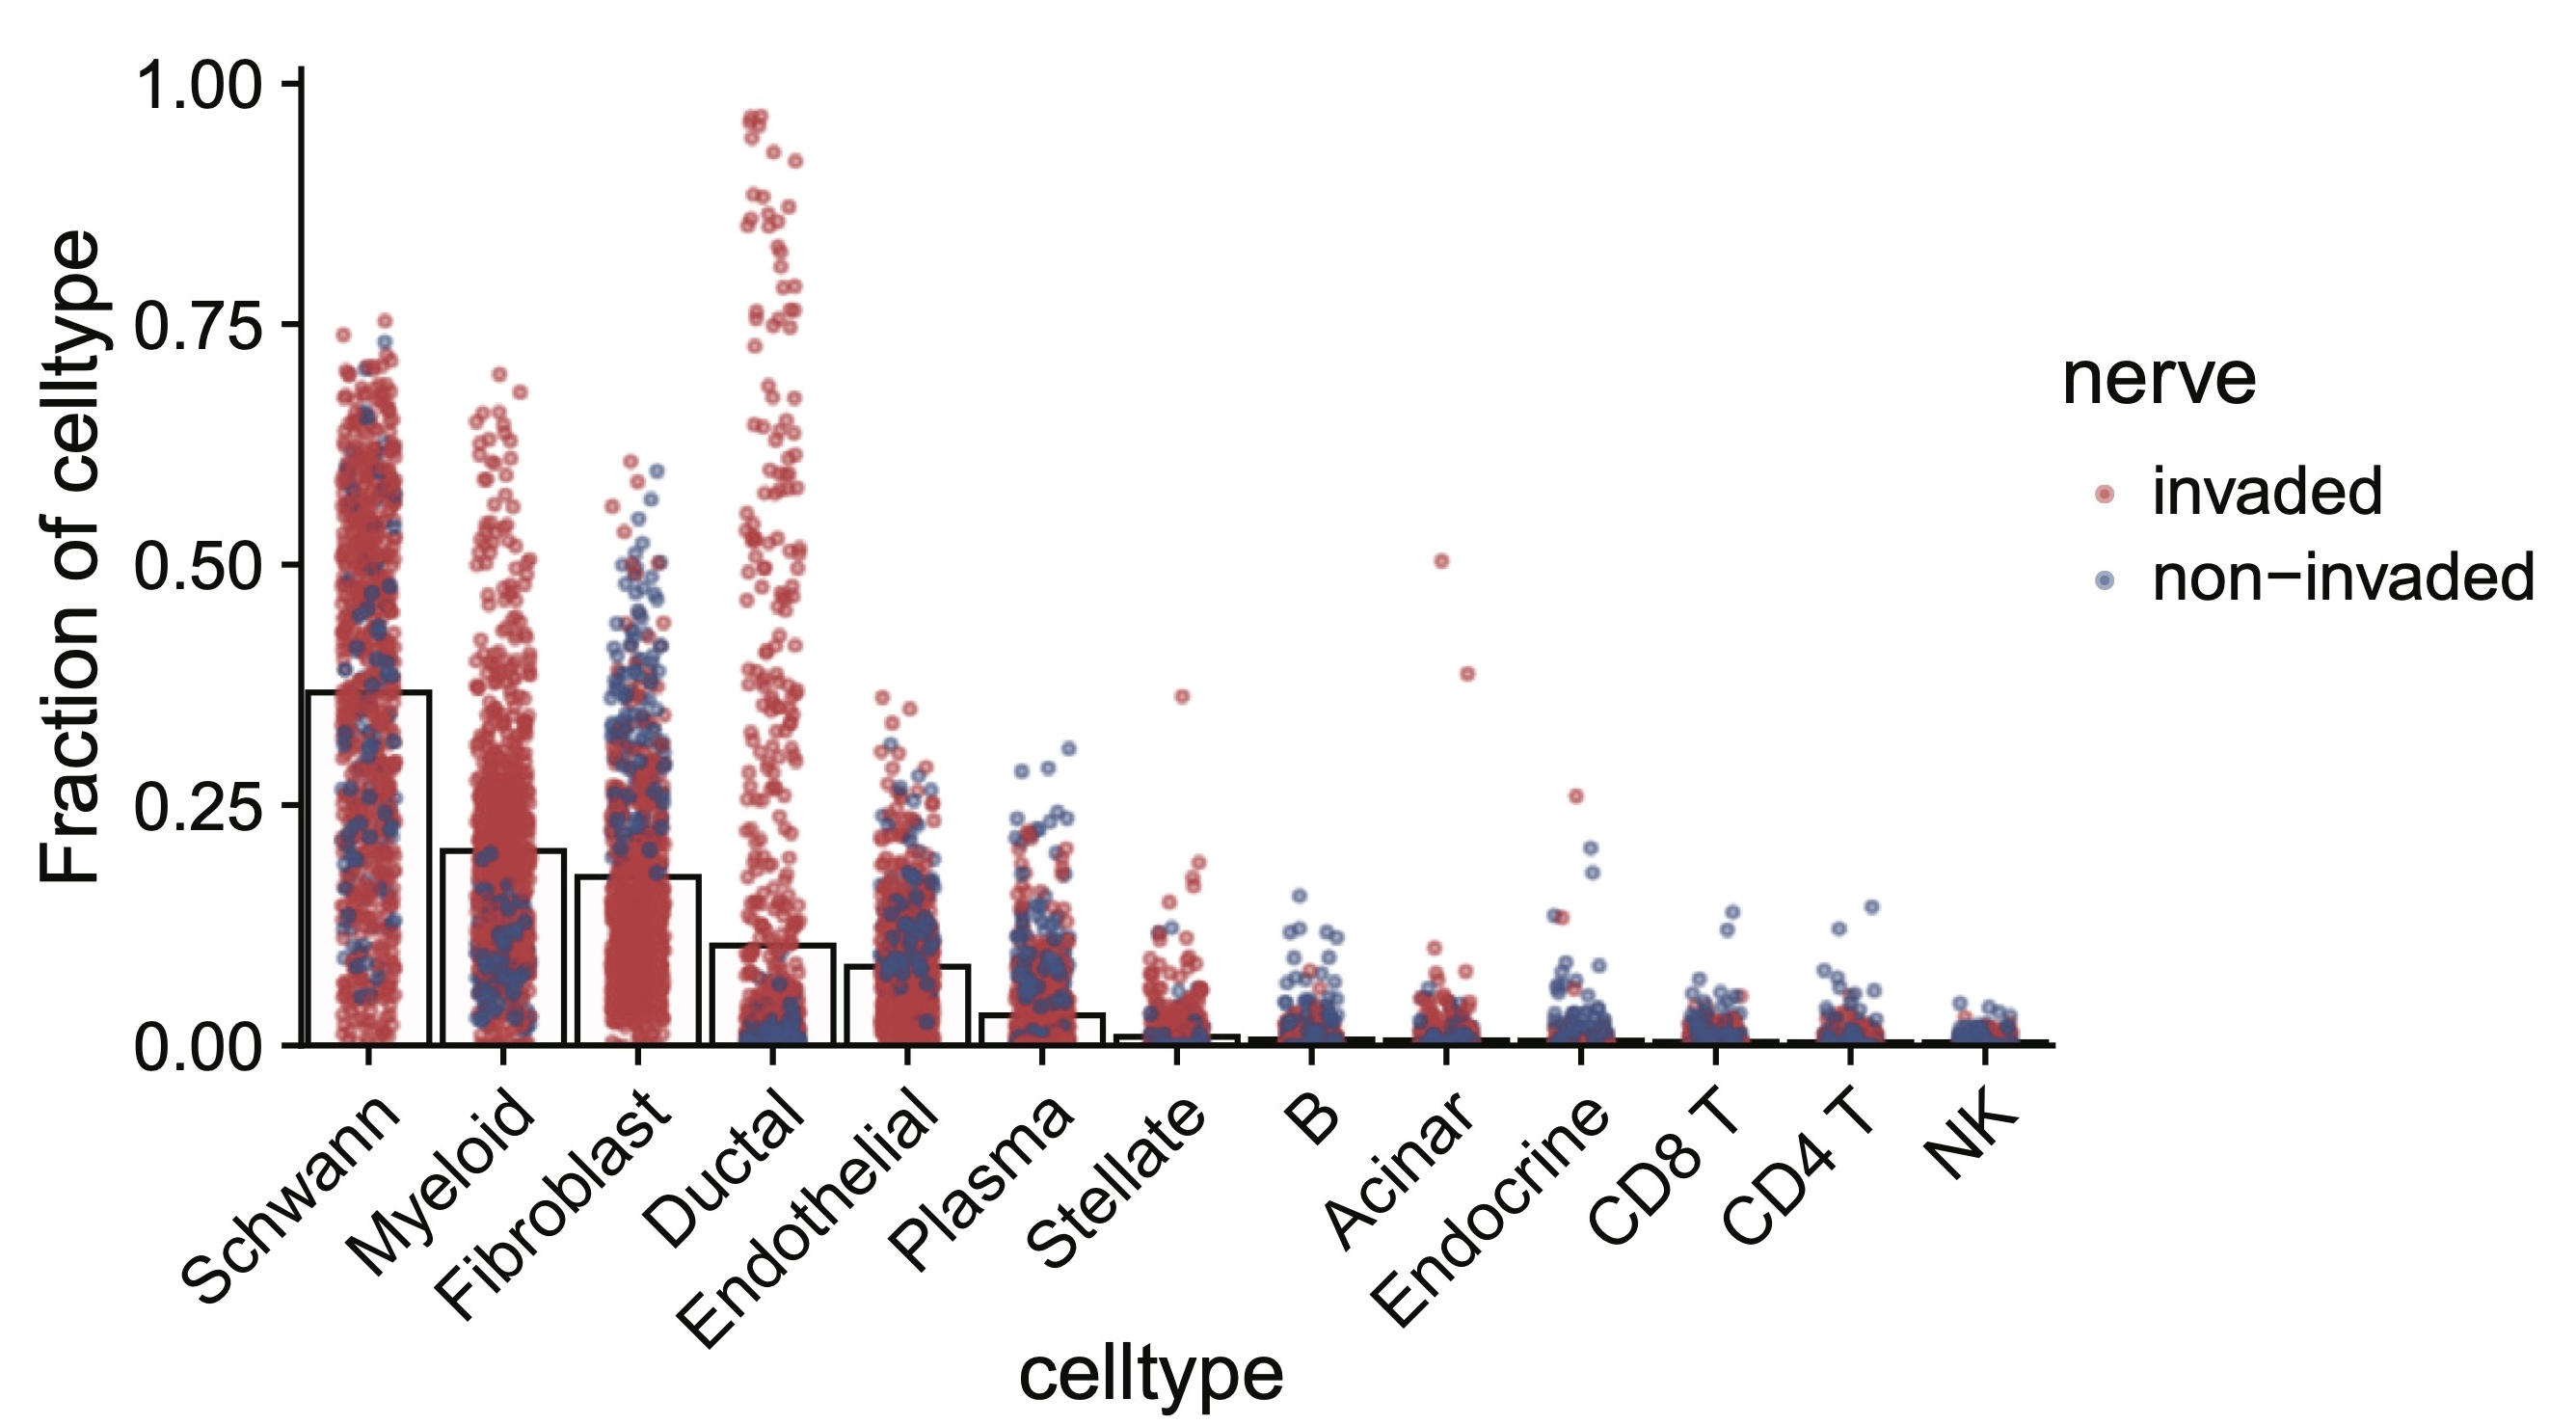
\includegraphics[width = 0.8\linewidth]{Figures/S6A.jpg}
  \end{figure}
  \begin{itemize}
    \item Nerve-resident stromal composition
      \begin{itemize}
        \item ST analysis determined that within tumor-associated nerves, \textbf{Schwann cells, myeloid cells and fibroblasts} are the three most abundant cell types.
      \end{itemize}
  \end{itemize}
\end{frame}

\begin{frame}{Endoneurial fibroblasts: F07\_Fibro-NRP2}
  \begin{itemize}
    \item Identification of a nerve-specific fibroblast subset
      \begin{itemize}
        \item Unsupervised clustering of sc/snRNA-seq revealed \textbf{F07\_Fibro-NRP2} as a fibroblast subset separated from other fibroblasts on UMAP.
        \item Shares LUM and DCN expression with other fibroblasts, but distinctly \textbf{upregulates axonogenesis-related genes}: NGFR, NRP2, AUTS2, RGMA.
      \end{itemize}
    \item Spatial localization and markers
      \begin{itemize}
        \item Projection onto ST data showed F07\_Fibro-NRP2 specifically located \textbf{inside nerves}.
        \item MISTy modelling revealed \textbf{strong spatial vicinity to Schwann cells}
              \(\Rightarrow\) a distinct \textbf{endoneurial fibroblast} subset.
        \item Endoneurial fibroblasts specially express APOD (lipoprotein), yielding APOD\(^{+}\)LUM\(^{+}\) fibroblasts in nerves, confirmed by mIHC.
      \end{itemize}
    \item Functional inference
      \begin{itemize}
        \item Pathway analysis suggests roles in \textbf{axonogenesis, regulation of stem cell differentiation, vasculogenesis and myeloid cell homeostasis}.
      \end{itemize}
  \end{itemize}
\end{frame}

\begin{frame}{Nerve-resident macrophages: from LYVE1\(^{+}\) to SPP1\(^{+}\)}
  \begin{itemize}
    \item Non-invaded nerves: \textbf{LYVE1\(^{+}\) tissue-resident macrophages}
      \begin{itemize}
        \item ST showed M08\_Macro-LYVE1 as the dominant myeloid subset in non-invaded nerves.
        \item Marked by LYVE1, FOLR2 and related genes, resembling \textbf{vessel-associated tissue-resident macrophages}.
        \item mIHC confirmed prevalent LYVE1\(^{+}\)CD68\(^{+}\) macrophages in non-invaded nerves.
      \end{itemize}
  \end{itemize}
  \begin{figure}
    \centering
    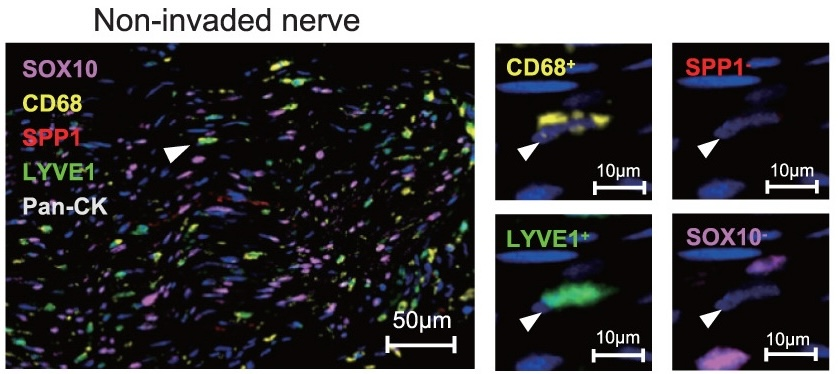
\includegraphics[width = 0.8\linewidth]{Figures/5Ft.jpg}
  \end{figure}
\end{frame}

\begin{frame}{Nerve-resident macrophages: from LYVE1\(^{+}\) to SPP1\(^{+}\)}
  \begin{itemize}
    \item Invaded nerves: \textbf{SPP1\(^{+}\) repair-like macrophages}
      \begin{itemize}
        \item Invaded nerves showed decreased M08\_Macro-LYVE1 and increased M10\_Macro-SPP1.
        \item M10\_Macro-SPP1 expresses high SPP1 (osteopontin) and TREM2; enriched in \textbf{synapse pruning, phagocytosis and angiogenesis regulation} pathways.
        \item Osteopontin is upregulated in \textbf{degenerating CNS microglia and promotes phagocytosis and myelination}.
        \item mIHC confirmed elevated SPP1\(^{+}\)CD68\(^{+}\) macrophages in invaded nerves.
      \end{itemize}
  \end{itemize}
  \begin{figure}
    \centering
    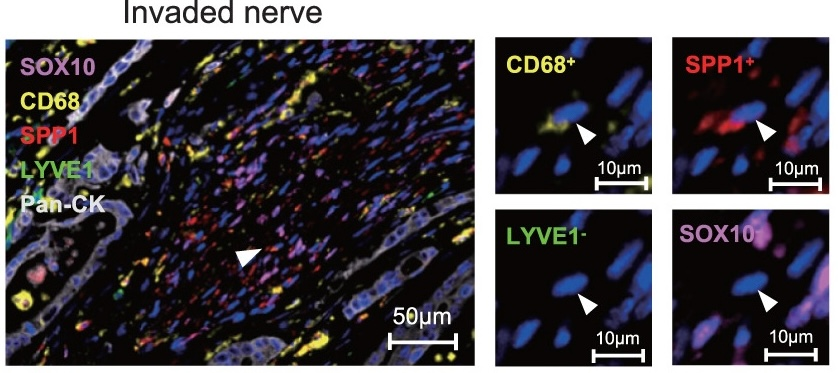
\includegraphics[width = 0.8\linewidth]{Figures/5Fb.jpg}
  \end{figure}
\end{frame}

\begin{frame}{Nerve-resident macrophages: from LYVE1\(^{+}\) to SPP1\(^{+}\)}
  \begin{itemize}
    \item \textbf{Trajectory and interpretation}
      \begin{itemize}
        \item RNA velocity and PAGA suggest \textbf{M10\_Macro-SPP1 may arise from M08\_Macro-LYVE1}.
        \item Monocyte infiltration into nerves is limited
              \(\Rightarrow\) nerve-resident macrophages likely \textbf{convert into repair-like SPP1\(^{+}\) macrophages} in response to cancer invasion.
        \item Further experiments are needed to validate these developmental trajectories and functions.
      \end{itemize}
  \end{itemize}
  \begin{columns}[T,onlytextwidth]
    \begin{column}{0.4\textwidth}
      \begin{figure}
        \centering
        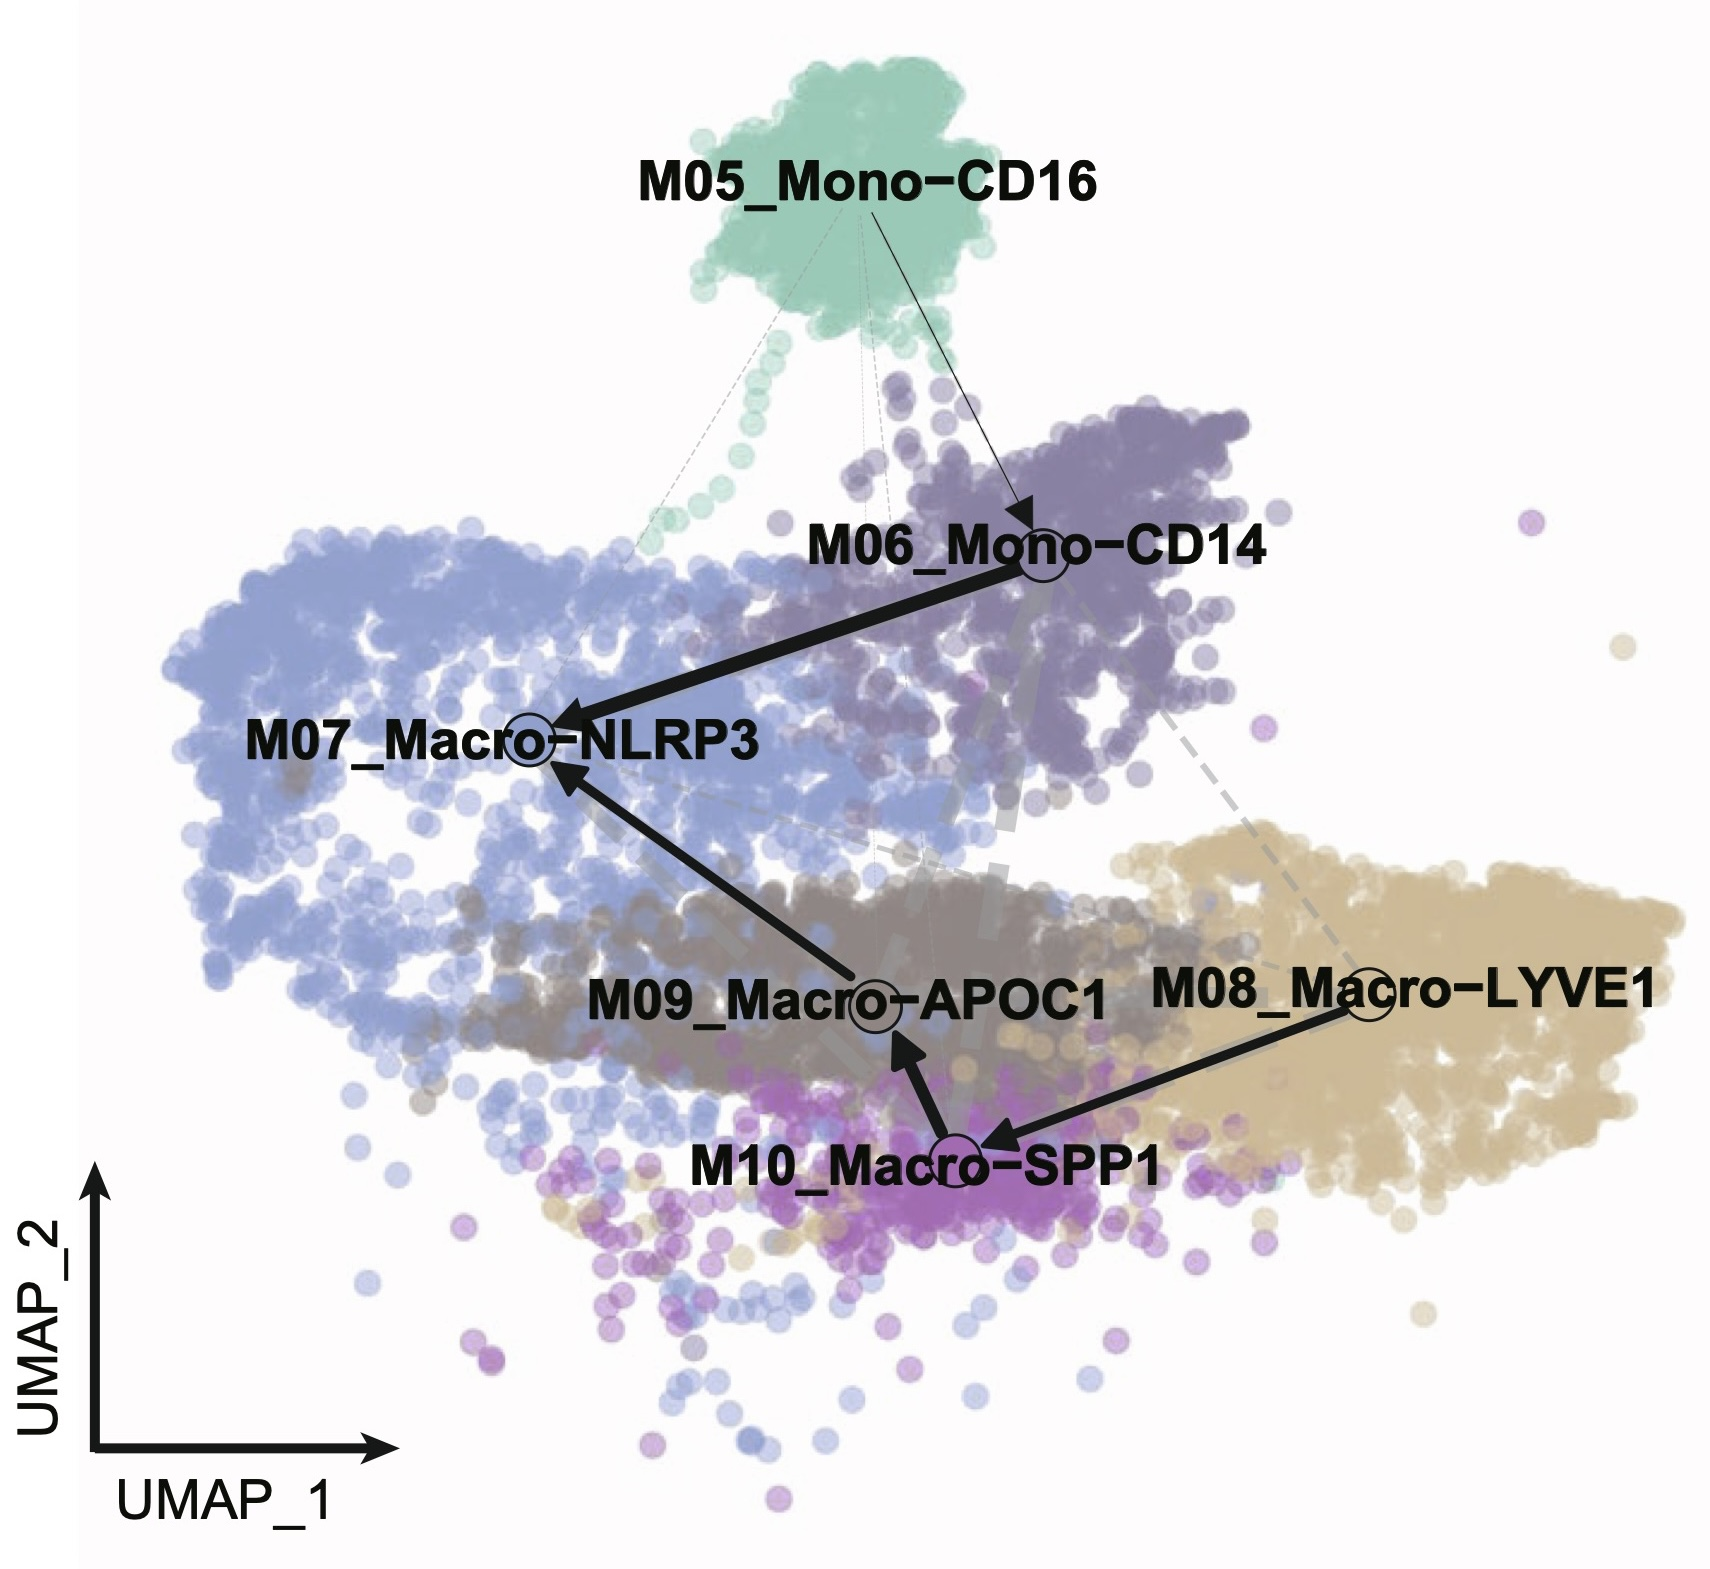
\includegraphics[width = 0.9\linewidth]{Figures/S6G.jpg}
      \end{figure}
    \end{column}
    \begin{column}{0.6\textwidth}
      \begin{figure}
        \centering
        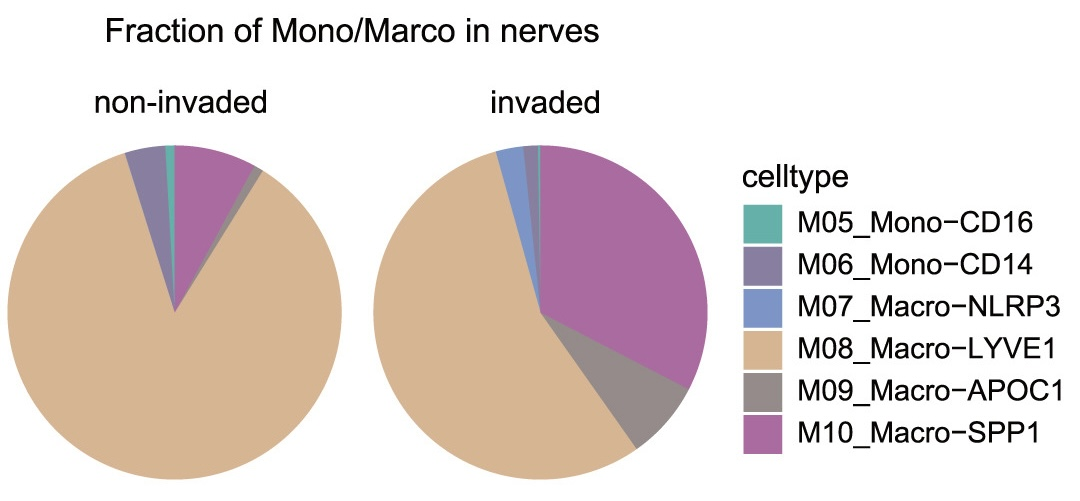
\includegraphics[width = 0.9\linewidth]{Figures/5E.jpg}
      \end{figure}
    \end{column}
  \end{columns}
\end{frame}

\begin{frame}{Part 3 Summary: Juxta-neural niches and nerve-resident cells}
  \begin{itemize}
    \item \textbf{Juxta-neural niches: protective TLS vs inflammatory niches}
      \begin{itemize}
        \item \textbf{Non-invaded nerves:} Juxta-neural regions enriched for \textbf{TLS components}; Frequent NTSs suggest a \textbf{tumor-associated, adaptive immune shield} supported by CXCL12-CXCR4 signaling.
        \item \textbf{Invaded nerves:} Juxta-neural regions show \textbf{increased IL-10 and TGF-\(\upbeta\) signaling}, higher \textbf{T cell exhaustion} marker expression, and \textbf{IL-1-driven innate inflammation}, forming a wound-like pro-invasive niche.
      \end{itemize}

    \item \textbf{Nerve-resident stromal and myeloid cells}
      \begin{itemize}
        \item Identified \textbf{F07\_Fibro-NRP2} as APOD\(^{+}\)LUM\(^{+}\) endoneurial fibroblasts enriched in axonogenesis, vasculogenesis and myeloid homeostasis pathways.
        \item Nerves harbor \textbf{LYVE1\(^{+}\) tissue-resident macrophages} (M08) in non-invaded states and \textbf{SPP1\(^{+}\)TREM2\(^{+}\) macrophages} (M10) in invaded states.
        \item Trajectory analysis suggests that \textbf{resident macrophages may convert into SPP1\(^{+}\) repair-like macrophages} upon cancer invasion, rather than being derived from infiltrating monocytes.
      \end{itemize}

    \item \textbf{Overall}
      \begin{itemize}
        \item Juxta-neural niches transition from \textbf{TLS-rich adaptive protection} to\textbf{innate inflammatory, immunosuppressive and stromally remodeled} environments as nerves become invaded in PDAC.
      \end{itemize}
  \end{itemize}
\end{frame}

%==================== Part 4 ====================%
\subsection{Part 4: Schwann cell heterogeneity and TGFBI\texorpdfstring{$^{+}$}{+} Schwann cells}

\begin{frame}{Part 4 Overview}
  \begin{itemize}
    \item Question: how do Schwann cell states contribute to neural invasion?
    \item Approach:
      \begin{itemize}
        \item Define Schwann subclusters from sc/snRNA-seq.
        \item Map their spatial distribution relative to tumor and nerves.
        \item Use computational ligand-receptor analysis and \textit{in vitro} assays to infer upstream signals and functional roles.
      \end{itemize}
    \item Key message:
      \begin{itemize}
        \item A distinct TGFBI\(^{+}\) Schwann subset (S02) is induced by TGF-\(\upbeta\)1 and promotes cancer cell migration and neural invasion.
      \end{itemize}
  \end{itemize}
\end{frame}

\begin{frame}{Schwann cell heterogeneity in PDAC}
  \begin{itemize}
    \item Unsupervised clustering of Schwann cells identified \textbf{three Schwann subsets}.

    \item \textbf{S01\_Schwann-ABCA8: myelinating Schwann cells}
      \begin{itemize}
        \item High expression of myelin-related genes: \textbf{MPZ}, \textbf{MBP}, \textbf{EGR2}.
        \item ABCA8 involved in \textbf{myelin synthesis} \(\Rightarrow\) \textbf{myelinating Schwann cell phenotype}.
      \end{itemize}

    \item \textbf{S02\_Schwann-TGFBI: ECM- and growth factor-rich subset}
      \begin{itemize}
        \item Lower myelin gene expression but higher \textbf{ECM genes}: FN1, COL12A1, CCN3, TGFBI.
        \item TGFBI can be induced by \textbf{TGF-\(\upbeta\)} signaling.
        \item Upregulated growth factors: \textbf{FGF5}, \textbf{MDK}, \textbf{BTC}
              \(\Rightarrow\) suggests a potential \textbf{pro-tumorigenic role}.
      \end{itemize}

    \item \textbf{S03\_Schwann-SERPINA3: repair-like Schwann cells}
      \begin{itemize}
        \item Express AP-1 family genes: \textbf{JUNB}, \textbf{JUND}, \textbf{FOS}, resembling \textbf{repair Schwann cells} in Bungner's bands (Schwann cell tubes that guide regenerating axons after peripheral nerve injury).
        \item Pathways enriched in \textbf{stress response}, regulation of endopeptidase activity and fibroblast proliferation
              \(\Rightarrow\) responds to injury and initiates repair signals.
      \end{itemize}
  \end{itemize}
\end{frame}

\begin{frame}{Spatial gradients of Schwann subsets and associated myeloid cells}
  \begin{itemize}
    \item Previous studies suggest that \textbf{Schwann cells could induce cancer cell migration and invasion}.
  \end{itemize}
  \vspace{-0.2cm}
  \begin{columns}[T,onlytextwidth]
    \begin{column}{0.6\textwidth}
      \begin{itemize}
        \item Spatial gradient from distant to tumor-adjacent nerve regions:
          \begin{itemize}
            \item Fraction of S02\_Schwann-TGFBI \textbf{increases toward tumor and invaded nerves}.
            \item Fraction of S01\_Schwann-ABCA8 decreases.
          \end{itemize}
      \end{itemize}
    \end{column}
    \begin{column}{0.4\textwidth}
      \begin{figure}
        \centering
        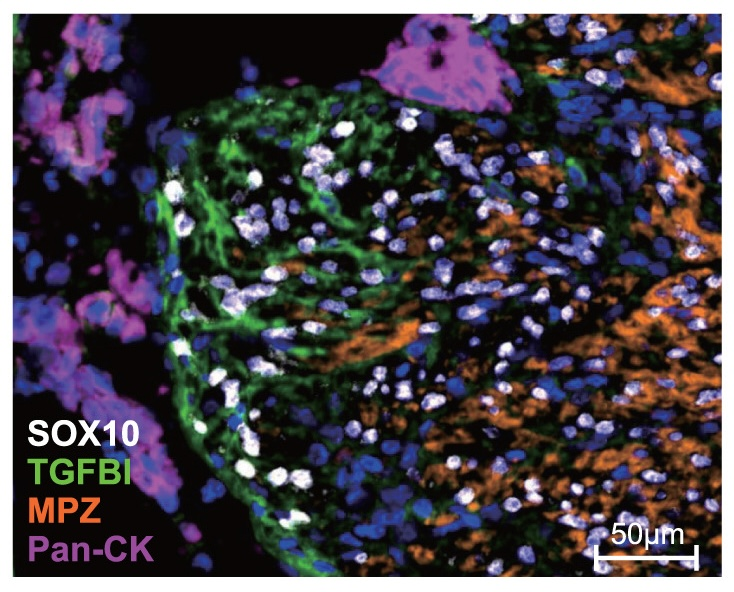
\includegraphics[width = 0.85\linewidth]{Figures/6C.jpg}
      \end{figure}
    \end{column}
  \end{columns}
  \vspace{-0.3cm}
  \begin{itemize}
    \item mIHC: TGFBI\(^{+}\) SOX10\(^{+}\) Schwann cells \textbf{align with invading cancer cells at the nerve edge}.
    \item Implication: Potential interaction between S02\_Schwann-TGFBI, invading cancer cells and the microenvironment at the invading edge.
  \end{itemize}
\end{frame}

\begin{frame}{Functional properties of S02\_Schwann-TGFBI}
  \begin{itemize}
    \item ECM remodeling and growth factor production
      \begin{itemize}
        \item Compared with S01 and S03, S02\_Schwann-TGFBI expresses higher levels of genes
              \textbf{constituting or regulating the ECM}, which can facilitate cell migration and metastasis.
        \item Upregulates multiple \textbf{growth factor-encoding genes}, potentially supporting
              cancer cell \textbf{survival and proliferation}.
      \end{itemize}

    \item Pathway analysis indicated enhanced activities in:
        \begin{itemize}
          \item Cadherin binding, focal adhesion, integrin-mediated signaling 
                \(\Rightarrow\) \textbf{strong adhesion and migration properties}.
          \item Regulation of neuron projection development, neuron migration, neuron-to-neuron synapse
                \(\Rightarrow\) \textbf{potential to guide neuron projections}.
        \end{itemize}
      \item Overall, S02\_Schwann-TGFBI may \textbf{create a favorable microenvironment} for cancer cell migration and invasion by ECM remodeling, matrix adhesion and neuro-guidance.
  \end{itemize}
\end{frame}

\begin{frame}{Experimental evidence of pro-migratory effects}
  \begin{columns}[T,onlytextwidth]
    \begin{column}{0.5\textwidth}
      \begin{itemize}
        \item Transwell migration assay:
        \begin{itemize}
          \item A pore-based co-culture system to quantify the tendency of cells migration.
          \item PDAC cells (e.g., PANC-1) show greater migration toward sNF96.2 Schwann cells / conditioned medium than control.
          \item Indicates S02-like Schwann cells \textbf{can attract and promote cancer cell migration}.
        \end{itemize}
      \end{itemize}
    \end{column}
    \begin{column}{0.5\textwidth}
      \begin{figure}
        \centering
        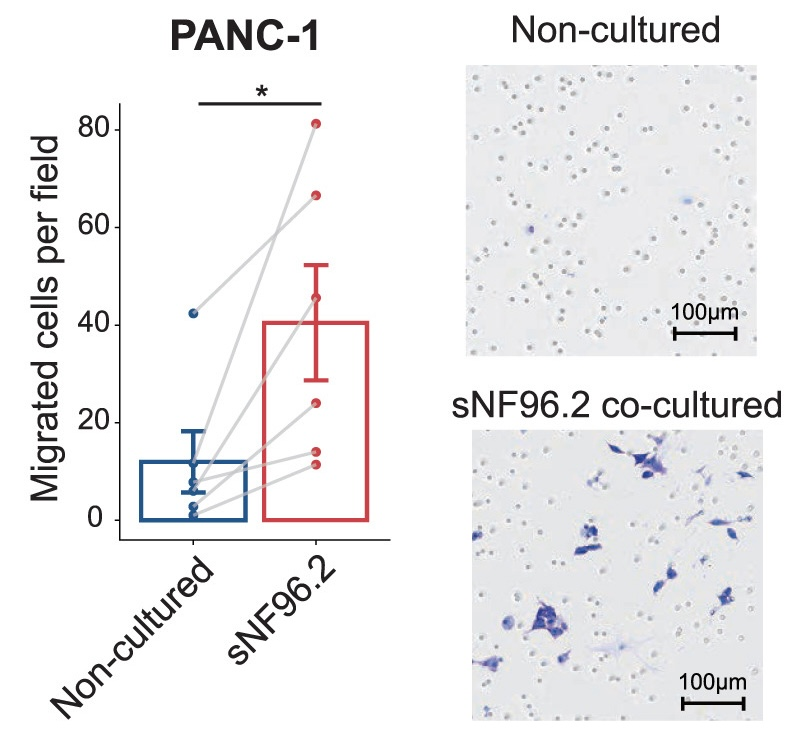
\includegraphics[width = 0.9\linewidth]{Figures/6E.jpg}
      \end{figure}
    \end{column}
  \end{columns}
  \begin{itemize}
    \item Schwann cell line model:
      \begin{itemize}
        \item RNA-seq demonstrates that sNF96.2 transcriptomic profiles \textbf{closely match S02\_Schwann-TGFBI} signatures, rather than S01 or S03.
      \end{itemize}
    \item \(\Rightarrow\) Supports that \textbf{S02-like Schwann cells actively promote cancer cell migration}.
  \end{itemize}
\end{frame}

\begin{frame}{Upstream signals shaping S02\_Schwann-TGFBI}
  \begin{itemize}
    \item Regulon analysis: TGF-\(\upbeta\)-linked transcription factors
      \begin{itemize}
        \item SCENIC-based regulon analysis on S02\_Schwann-TGFBI revealed distinct activity of
              \textbf{RUNX1}, \textbf{TFAP2A} and \textbf{SMAD1}.
        \item These transcription factors are known to participate in \textbf{TGF-\(\upbeta\) signaling},
              suggesting that S02\_Schwann-TGFBI is shaped by microenvironmental TGF-\(\upbeta\) cues.
      \end{itemize}

    \item Candidate inducing cytokines
      \begin{itemize}
        \item CytoSig and NicheNet were used to predict upstream ligands regulating the S02 signature.
        \item \textbf{TGF-\(\upbeta\)1} and \textbf{HGF} ranked among the top candidate factors.
      \end{itemize}
  \end{itemize}
  \begin{figure}
    \centering
    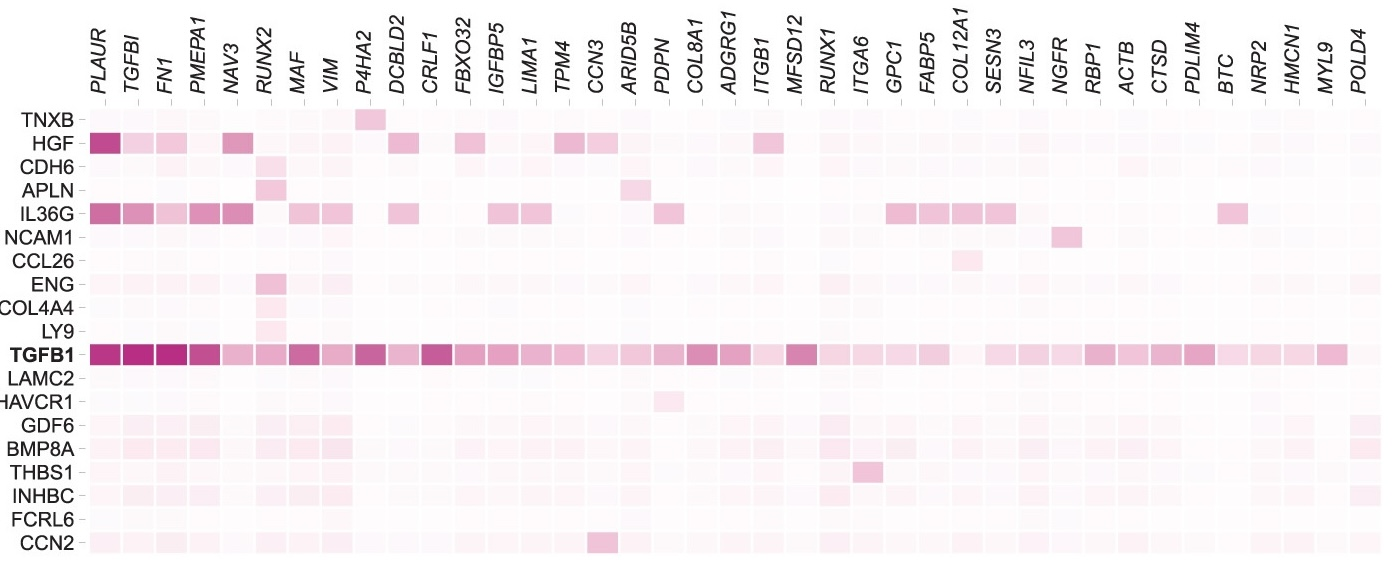
\includegraphics[width = 0.7\linewidth]{Figures/6G.jpg}
  \end{figure}
\end{frame}

\begin{frame}{Upstream signals shaping S02\_Schwann-TGFBI}
  \begin{figure}
    \centering
    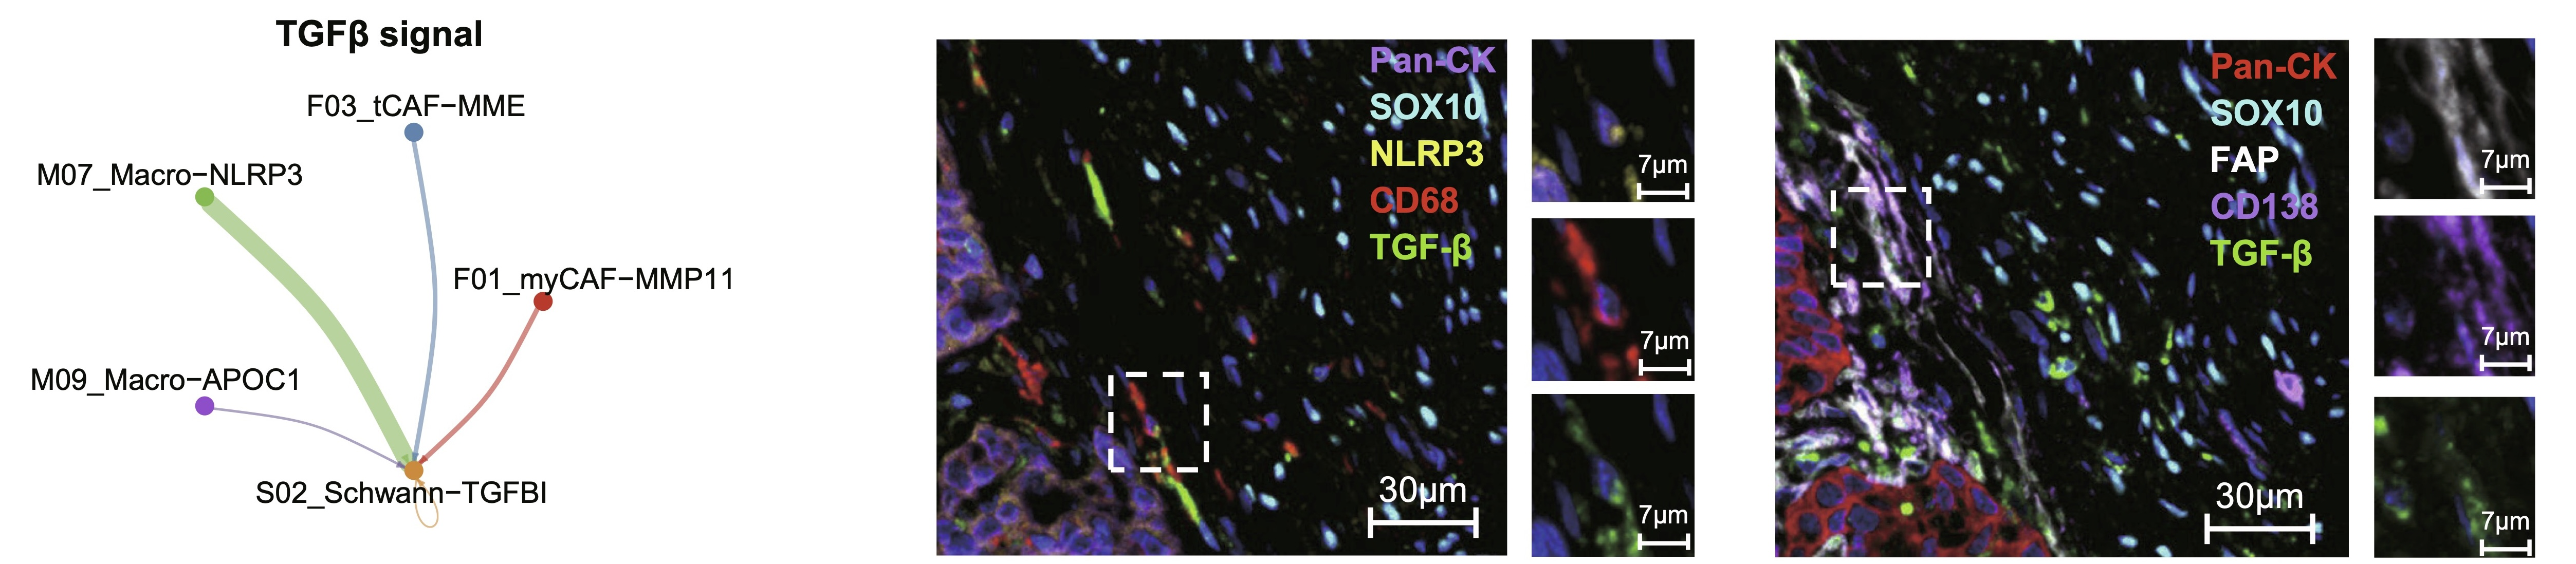
\includegraphics[width = 0.9\linewidth]{Figures/S7F&G.jpg}
  \end{figure}
  \begin{itemize}
    \item \textbf{TGF-\(\upbeta\)1 sources around invaded nerves}
      \begin{itemize}
        \item Four subsets enriched in high-NI tumors and adjacent to invaded nerves:
              \textbf{M07\_Macro-NLRP3}, M09\_Macro-APOC1, \textbf{F01\_myCAF-MMP11}, F03\_tCAF-MME.
        \item All can potentially produce TGF-\(\upbeta\)1, with \textbf{M07} and \textbf{F01} as major contributors
              (higher expression and/or greater cell proportions).
        \item CellChat analysis shows strong \textbf{TGF-\(\upbeta\) signaling from M07 and F01 to S02\_Schwann-TGFBI}.
        \item mIHC confirms TGF-\(\upbeta\)1 expression by \textbf{NLRP3\(^{+}\) TAMs} and \textbf{myCAFs}.
      \end{itemize}

    \item \textbf{HGF less likely to be dominant}
      \begin{itemize}
        \item HGF is barely expressed by cells adjacent to invaded nerves, arguing against a major role in S02 induction.
      \end{itemize}

    \item \(\Rightarrow\) S02\_Schwann-TGFBI is likely \textbf{induced by TGF-\(\upbeta\)1} produced from \textbf{M07\_Macro-NLRP3} and \textbf{F01\_myCAF-MMP11} around invaded nerves.
  \end{itemize}
\end{frame}

\begin{frame}{\textit{In vitro} validation of TGF-\(\upbeta\)1 induction of TGFBI\(^{+}\) Schwann cells}
  \begin{itemize}
    \item TGF-\(\upbeta\)1 reprograms Schwann cells toward S02-like state
      \begin{itemize}
        \item Recombinant human TGF-\(\upbeta\)1 treatment of sNF96.2 Schwann cells: \(\uparrow\) S02 markers: TGFBI, FN1; \(\downarrow\) S01 marker: ABCA8.
        \item Selective TGF-\(\upbeta\)RI inhibitor SB505124 \(\Rightarrow\) \textbf{abrogates} these transcriptional changes.
        \item ELISA confirms increased \textbf{TGFBI protein expression and secretion}.
      \end{itemize}

    \item TGF-\(\upbeta\)1-treated Schwann cells promote PDAC cell migration \& invasion
      \begin{itemize}
        \item \textbf{Transwell assays}:
          \begin{itemize}
            \item PANC-1 shows \textbf{greater migration and invasion} toward TGF-\(\upbeta\)1-treated sNF96.2 than control. Effect is \textbf{blocked} by SB505124.
          \end{itemize}
        \end{itemize}
  \end{itemize}
  \vspace{-0.3cm}
  \begin{figure}
    \centering
    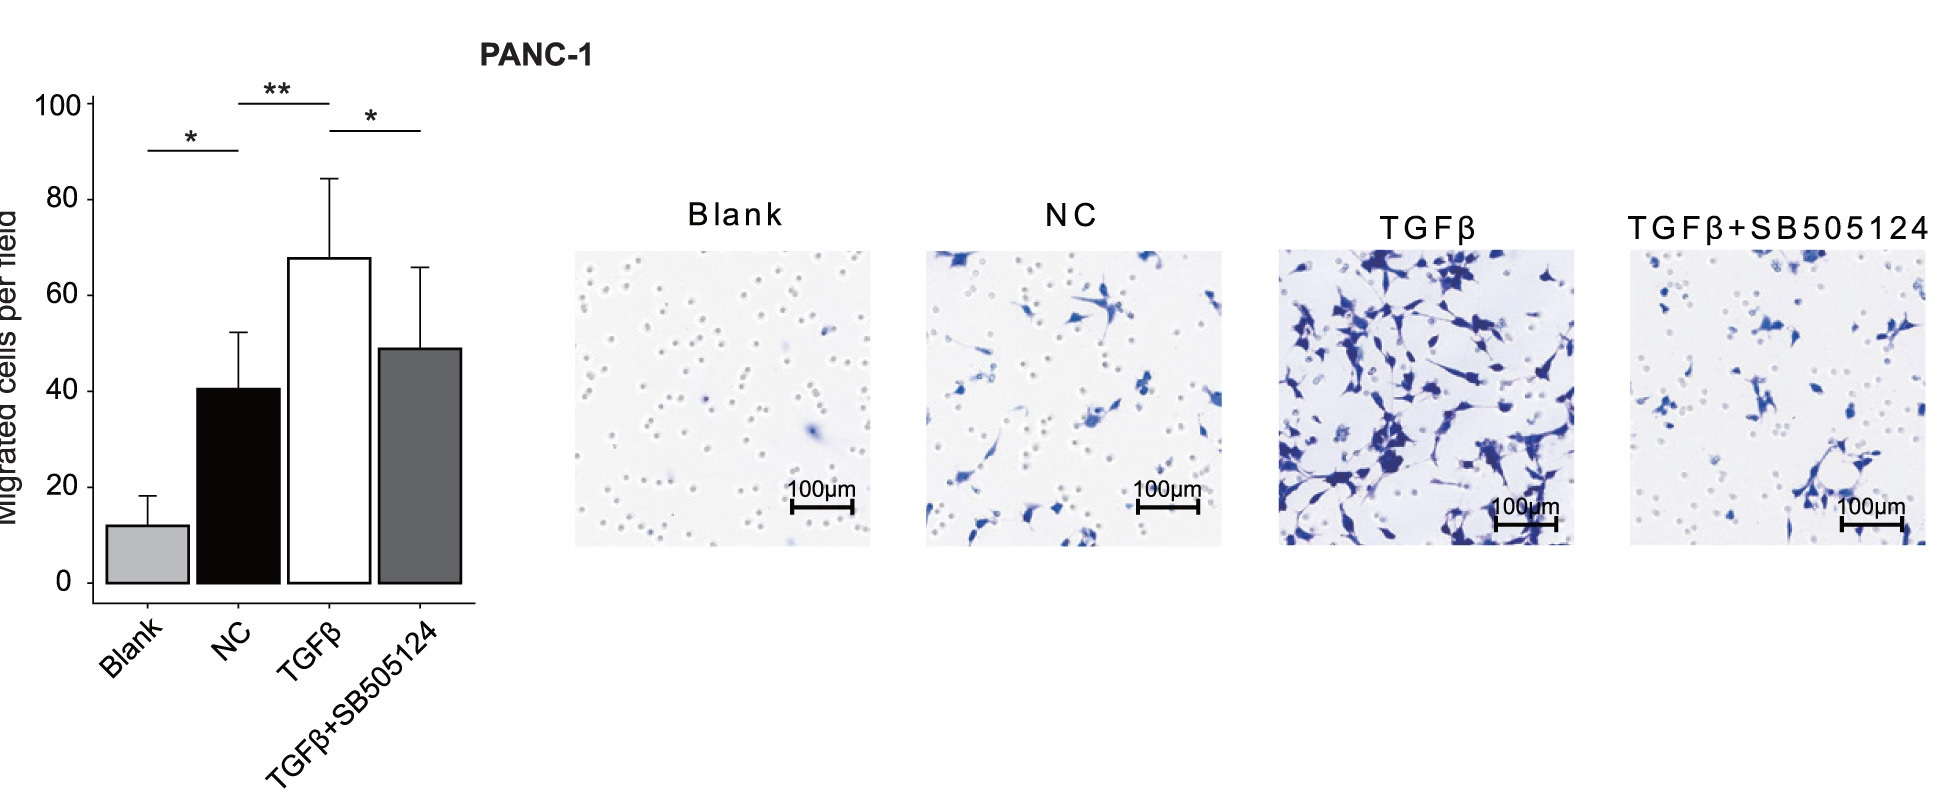
\includegraphics[width = 0.8\linewidth]{Figures/6J.jpg}
  \end{figure}
\end{frame}

\begin{frame}{\textit{In vitro} validation of TGF-\(\upbeta\)1 induction of TGFBI\(^{+}\) Schwann cells}
  \begin{itemize}
    \item TGF-\(\upbeta\)1-treated Schwann cells promote PDAC cell migration \& invasion
      \begin{itemize}
        \item \textbf{Wound healing assays}:
          \begin{itemize}
            \item Supernatant from TGF-\(\upbeta\)1-treated sNF96.2 accelerates PANC-1 migration. Red lines delineate the wound.
          \end{itemize}
      \end{itemize}
    \end{itemize}
    \begin{figure}
      \centering
      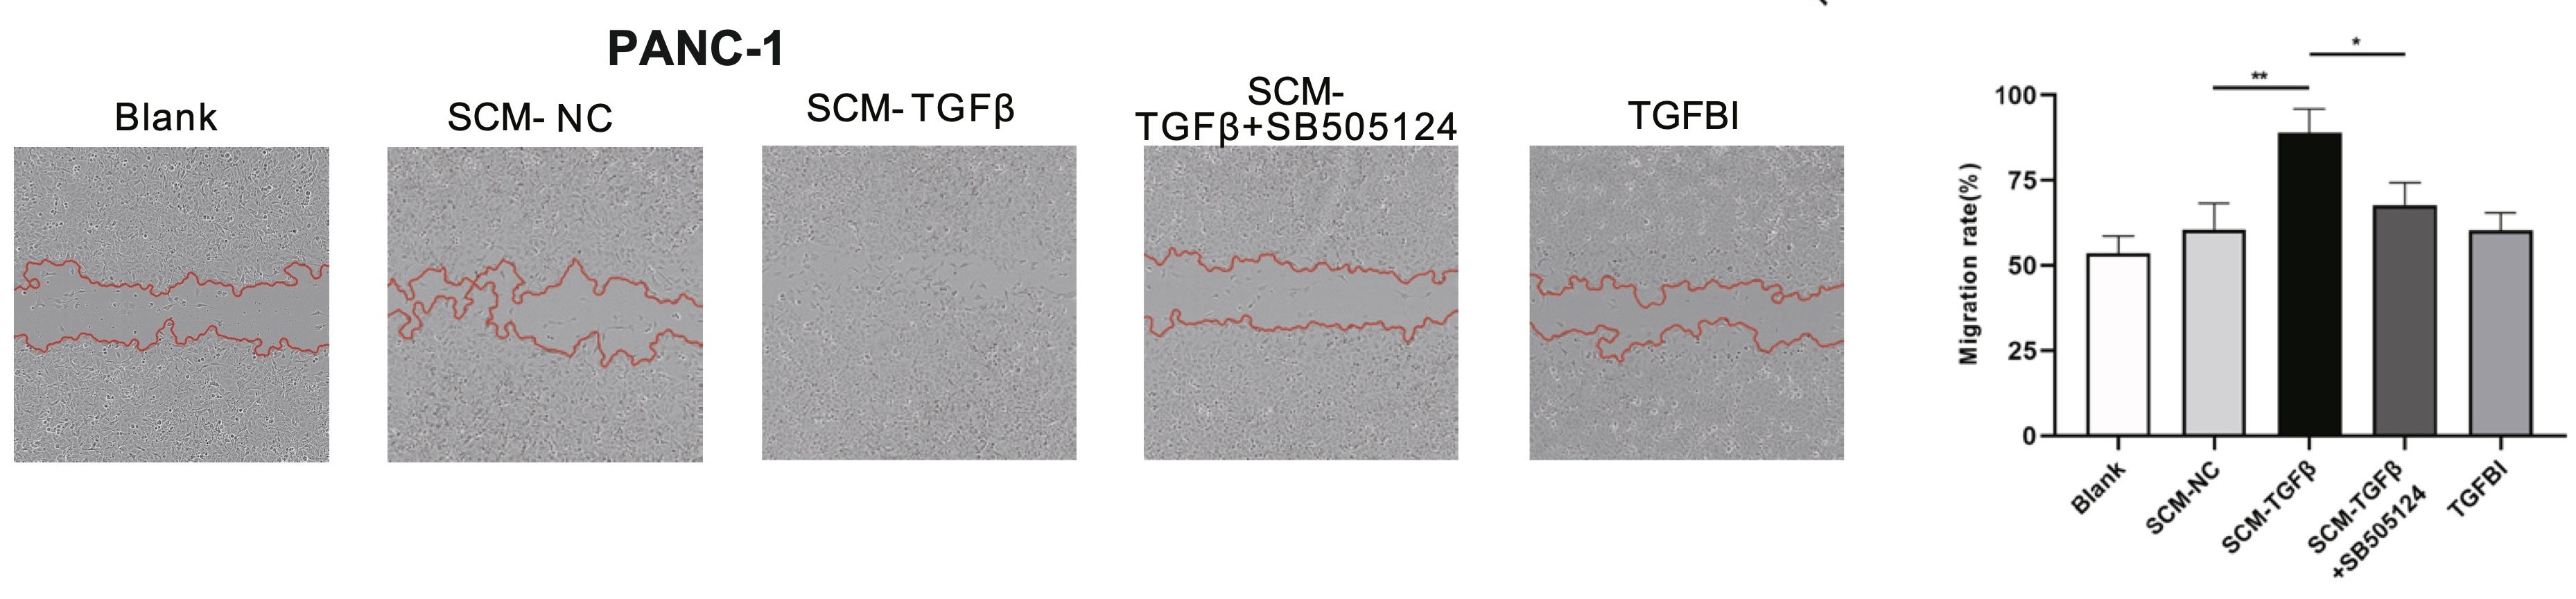
\includegraphics[width = 0.9\linewidth]{Figures/S8C.jpg}
    \end{figure}
\end{frame}

\begin{frame}{\textit{In vitro} validation of TGF-\(\upbeta\)1 induction of TGFBI\(^{+}\) Schwann cells}
  \begin{itemize}
    \item TGF-\(\upbeta\)1-treated Schwann cells promote PDAC cell migration \& invasion
      \begin{itemize}
        \item \textbf{Random migration assays}:
          \begin{itemize}
            \item Conditioned medium from TGF-\(\upbeta\)1-treated sNF96.2 increases \textbf{velocity} and \textbf{accumulated distance} of PANC-1 and MIA PaCa-2 cells.
          \end{itemize}
      \end{itemize}
    \item TGFBI protein shows \textbf{minimal effect} in these assays.
    \item \(\Rightarrow\) TGF-\(\upbeta\)1-induced Schwann cell state (not TGFBI alone) drives pro-migratory effects.
  \end{itemize}
  \begin{figure}
    \centering
    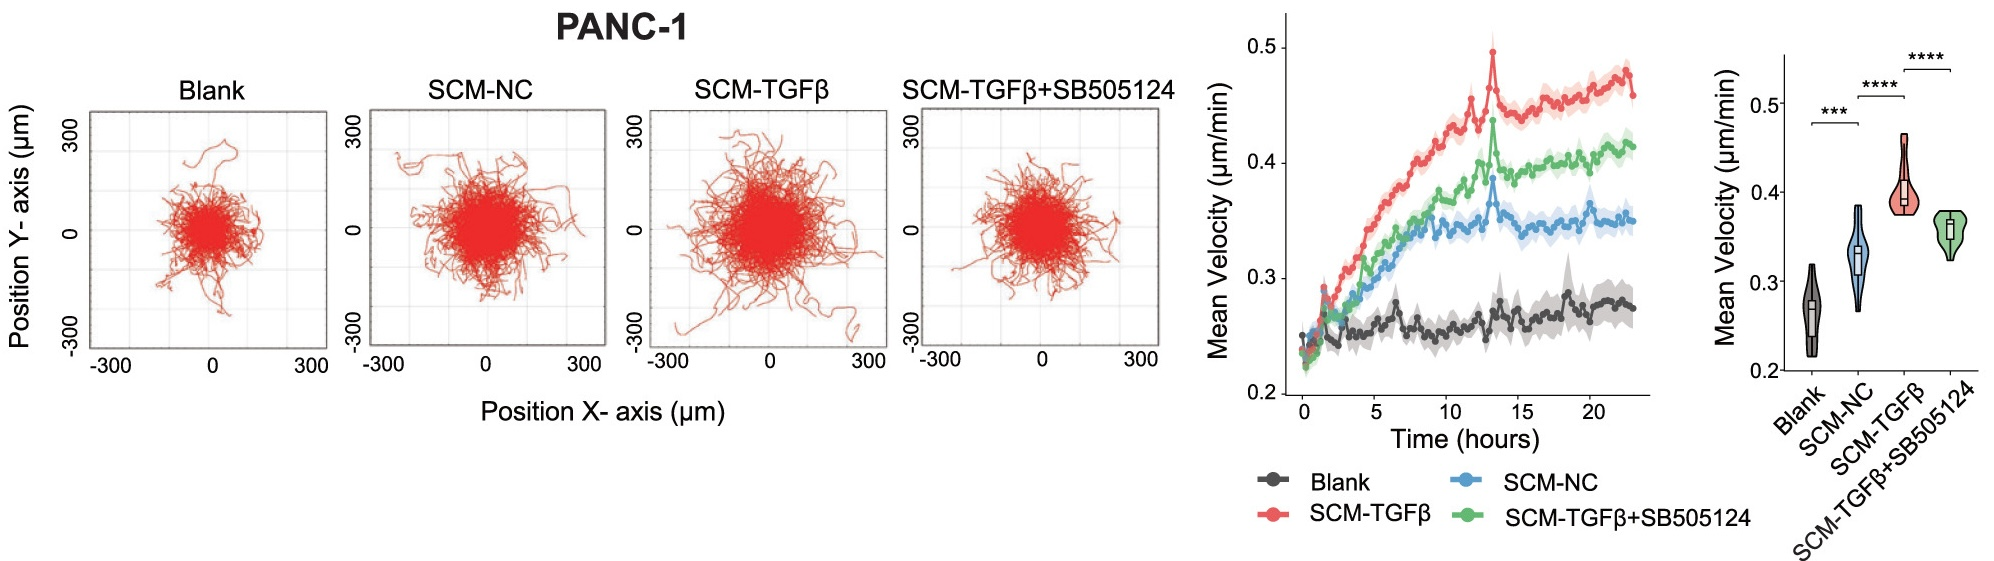
\includegraphics[width = 0.9\linewidth]{Figures/6K.jpg}
  \end{figure}
\end{frame}

\begin{frame}{Part 4 Summary: TGFBI\(^+\) Schwann subset induced by TGF-\(\upbeta\)1 promotes neural invasion}
  \begin{itemize}
    \item Schwann cell states:
      \begin{itemize}
        \item S01\_Schwann-ABCA8: myelinating, homeostatic.
        \item S02\_Schwann-TGFBI: TGF-\(\upbeta\)-driven transforming state with ECM-remodeling and pro-invasive features.
        \item S03\_Schwann-SERPINA3: stress/inflammation-associated.
      \end{itemize}
    \item High-NI context:
      \begin{itemize}
        \item Pro-inflammatory macrophages (M07) and myCAFs (F01) around invaded nerves secrete TGF-\(\upbeta\)1.
        \item TGF-\(\upbeta\)1 induces S02\_Schwann-TGFBI, which in turn promotes cancer cell migration and nerve invasion.
      \end{itemize}
    \item Integrated model of NI in PDAC:
      \begin{itemize}
        \item Intrinsic: basal-like CEACAM6\(^{+}\) and GABRP\(^{+}\) malignant cells have high NI potential.
        \item Microenvironmental: loss of TLS-rich protective niches and gain of inflammatory, CAF- and TGFBI\(^{+}\) Schwann cell-rich niches drive neural invasion.
      \end{itemize}
  \end{itemize}
\end{frame}

\section{Discussion, Evaluation \& Implication}

\subsection{Discussion}

\begin{frame}{Discussion I: Key Findings}
  \begin{itemize}
    \item \textbf{Built an integrated single-cell and spatial atlas of PDAC with different neural invasion (NI) statuses, resolving the cellular composition and organization around nerves.}
  \end{itemize}
  \begin{figure}
    \centering
    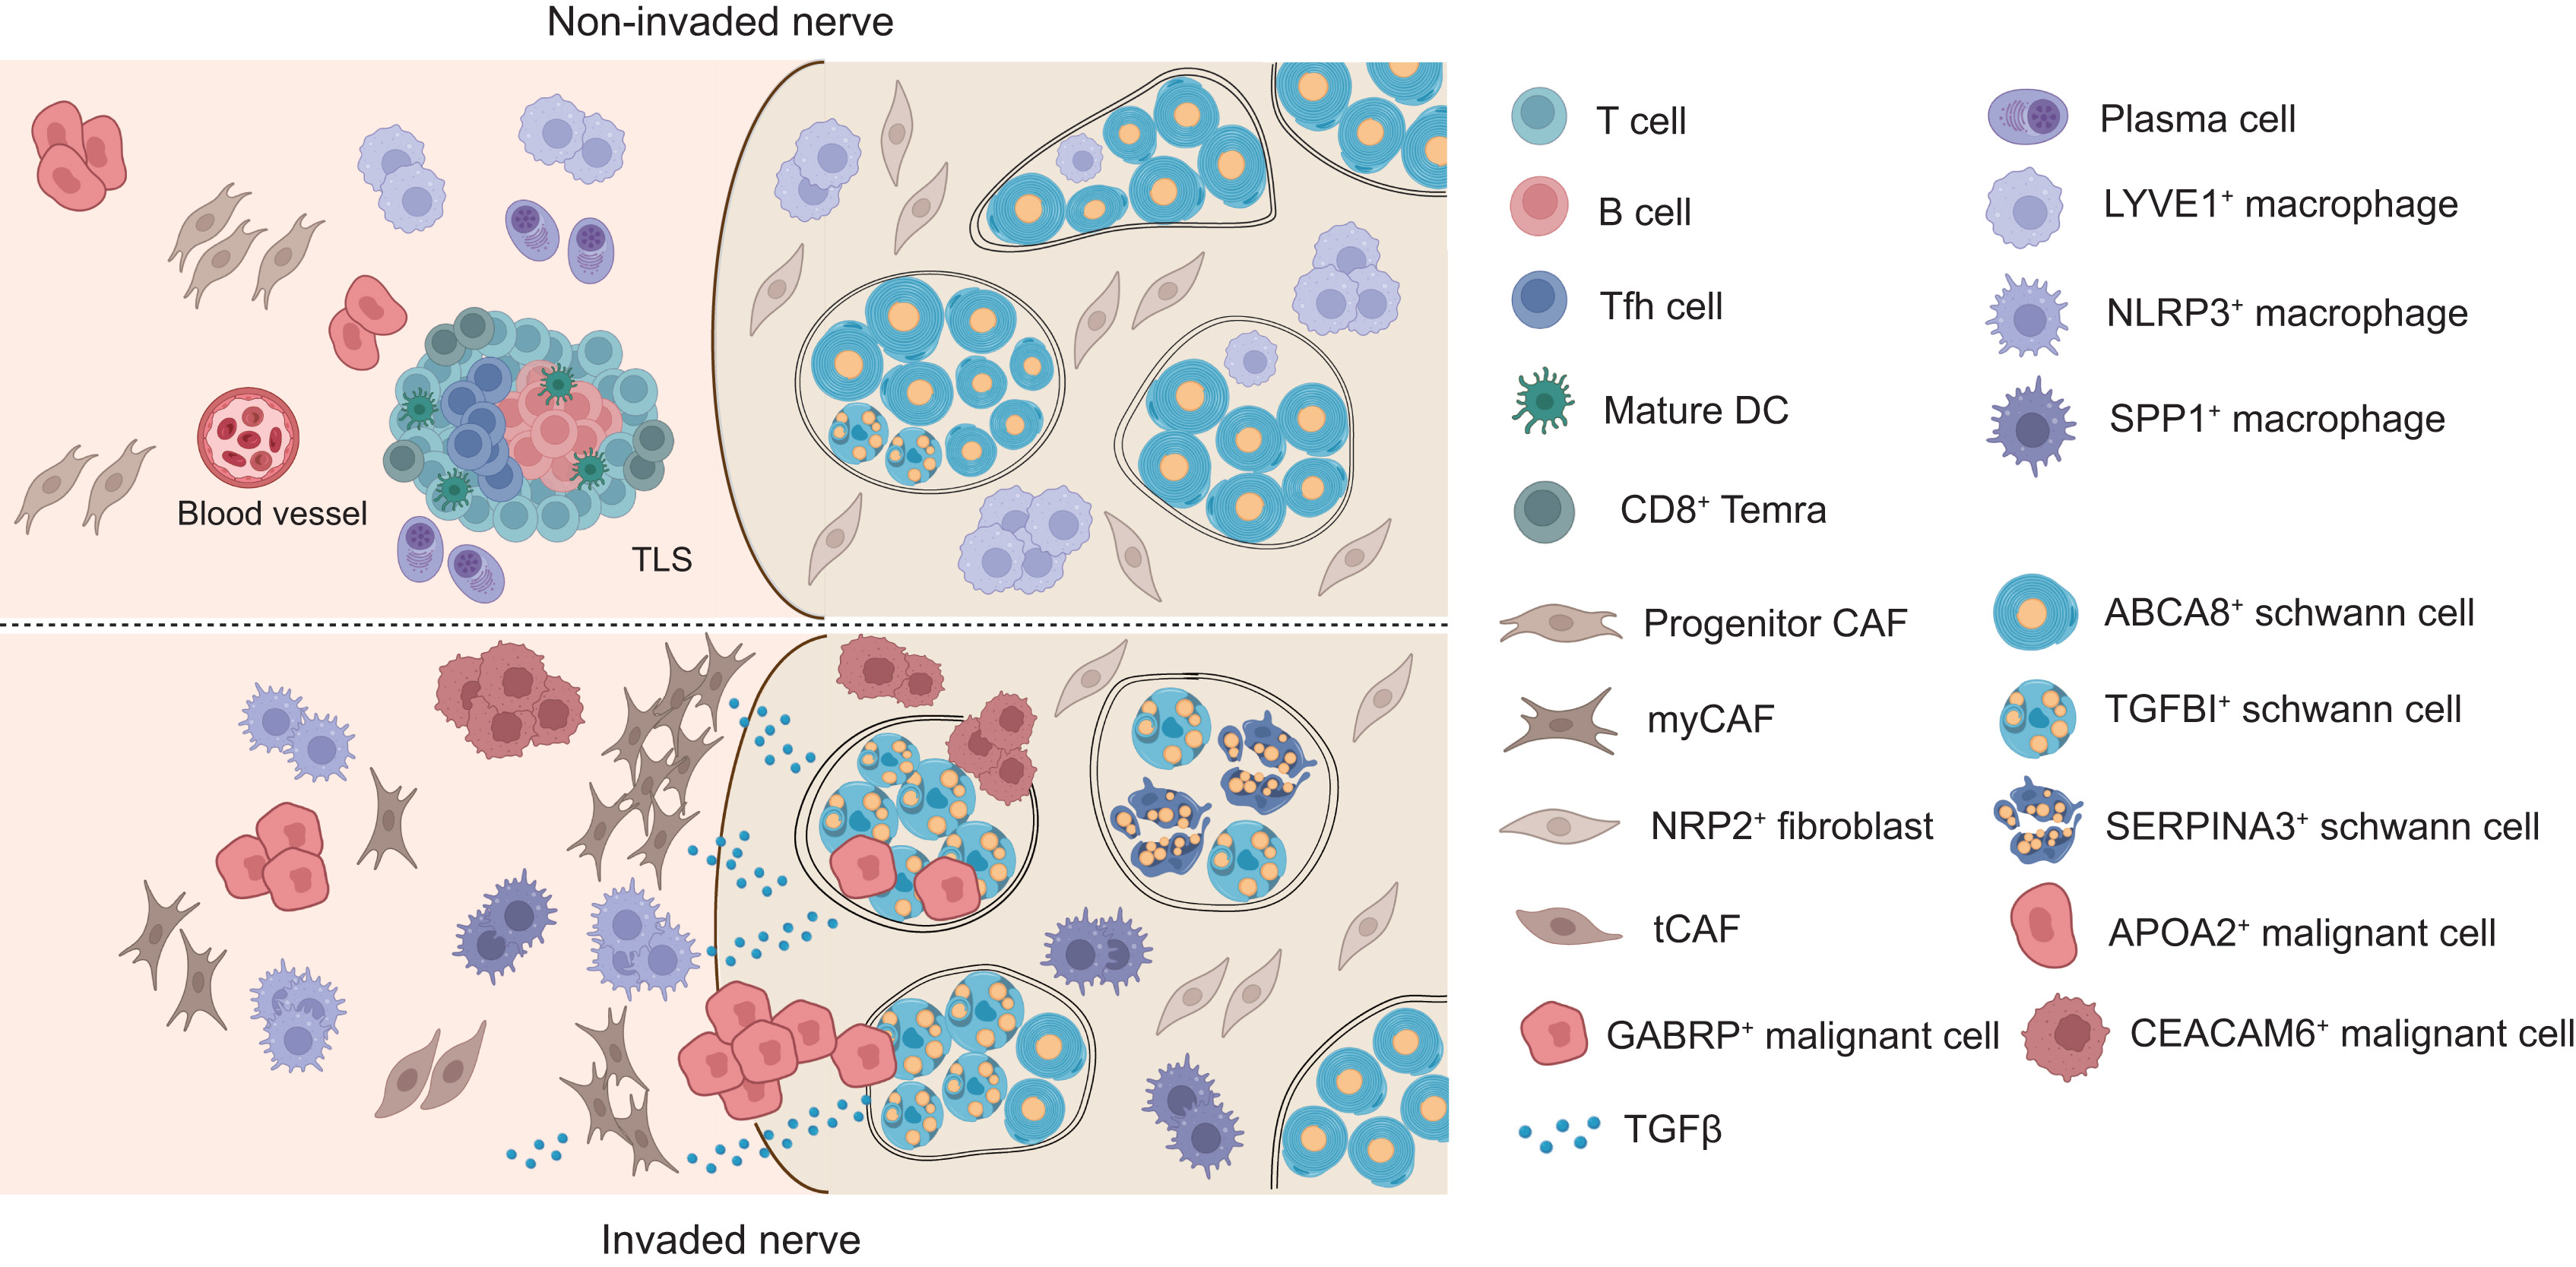
\includegraphics[width = 0.9\linewidth]{Figures/7.jpg}
  \end{figure}
\end{frame}

\begin{frame}{Discussion I: Key Findings}
  \begin{itemize}
    \item \textbf{Identified a novel intraneural fibroblast subset (F07\_Fibro-NRP2):}
      \begin{itemize}
        \item Enriched for axonogenesis- and neurogenesis-related genes.
        \item Preferentially localized inside nerves.
        \item High APOD expression suggests a role in mitigating oxidative stress and supporting neuronal integrity.
      \end{itemize}
    \item \textbf{Revealed marked heterogeneity of Schwann cells:}
      \begin{itemize}
        \item S01\_Schwann-ABCA8: myelinating-like Schwann cells.
        \item S03\_Schwann-SERPINA3: repair-like Schwann cells.
        \item S02\_Schwann-TGFBI: distinct, ECM- and growth factor-rich subset associated with NI.
      \end{itemize}
    \item External datasets and \textit{in vitro} assays support that \textbf{TGF-\(\upbeta\)1 drives the induction of S02-like TGFBI\(^+\) Schwann cells and enhances PDAC cell migration and invasion.}
  \end{itemize}
\end{frame}

\begin{frame}{Discussion II: Mechanistic Model and Implications}
  \begin{itemize}
    \item At the invasive neural front, \textbf{myCAF and NLRP3\(^+\) TAMs are enriched, while LYVE1\(^+\) tissue-resident macrophages and progenitor-like CAFs are depleted}.
    \item \textbf{MyCAF and NLRP3\(^+\) TAMs produce high levels of TGF-\(\upbeta\)1:}
      \begin{itemize}
        \item Strengthened TGF-\(\upbeta\) signaling around invaded nerves.
        \item Promotes reprogramming of Schwann cells toward the S02\_Schwann-TGFBI phenotype.
      \end{itemize}
    \item \textbf{Identified NI-associated malignant ductal subsets:}
      \begin{itemize}
        \item D09\_Ductal-CEACAM6 resembles previously reported “transition/basal-like” high-NI states.
        \item D04\_Ductal-GABRP shows a nerve-responsive transcriptional program, indicating multiple routes to acquire neuro-invasive potential.
      \end{itemize}
    \item Broader implications:
      \begin{itemize}
        \item Provides a human PDAC nerve-centric atlas to guide future targeting of specific stromal and immune subsets at the NI front.
        \item Offers a framework for dissecting neuro-immune-tumor interactions and for designing neural or psychological interventions in cancer.
      \end{itemize}
  \end{itemize}
\end{frame}

\subsection{Evaluation}

\begin{frame}{Strengths of the Study}
  \begin{itemize}
    \item \textbf{Multi-modal design}
      \begin{itemize}
        \item Integrates sc/snRNA-seq, spatial transcriptomics, mIHC, and \textit{in vitro} functional assays.
        \item Enables cross-validation of cell states and spatial patterns around neural invasion (NI).
      \end{itemize}
    \item \textbf{Focus on neural invasion microenvironment}
      \begin{itemize}
        \item Explicitly defines NI-high vs NI-low tumors and juxta-neural regions.
        \item Dissects malignant, Schwann, myeloid, and fibroblast subtypes in NI context rather than globally.
      \end{itemize}
    \item \textbf{Comprehensive cell-state annotation}
      \begin{itemize}
        \item Multiple malignant ductal subtypes, distinct Schwann clusters (including TGFBI\textsuperscript{+}), diverse macrophage and CAF subsets.
        \item Combines CNV inference, gene signatures, and pathway scores for annotation.
      \end{itemize}
  \end{itemize}
\end{frame}

\begin{frame}{Strengths of the Study}
  \begin{itemize}
    \item \textbf{Spatially resolved analyses}
      \begin{itemize}
        \item Uses spatial transcriptomics and NI-focused regions to map gradients of cell states around invaded nerves.
        \item Correlates Schwann and myeloid subsets with NI severity and nerve distance.
      \end{itemize}
    \item \textbf{Network and communication analysis}
      \begin{itemize}
        \item Applies tools such as network modeling (e.g., MistyR) and ligand-receptor analysis (e.g., CellChat/others).
        \item Identifies candidate signaling axes between malignant cells, Schwann cells, macrophages, and CAFs.
      \end{itemize}
    \item \textbf{Functional validation}
      \begin{itemize}
        \item \textit{In vitro} experiments support a role of TGF-\(\upbeta\) in inducing TGFBI\textsuperscript{+} Schwann phenotype.
        \item Conditioned media and co-culture assays show enhanced PDAC migration/invasion toward TGF-\(\upbeta\)-stimulated Schwann cells.
      \end{itemize}
  \end{itemize}
\end{frame}

\begin{frame}{Limitations and Potential Biases}
  \begin{itemize}
    \item \textbf{Cohort size and representativeness}
      \begin{itemize}
        \item Moderate patient numbers; single-center, mainly one population.
        \item May limit generalizability across ethnicities, treatment backgrounds, or earlier disease stages.
      \end{itemize}
    \item \textbf{Cross-sectional design}
      \begin{itemize}
        \item All samples taken at surgery; no longitudinal sampling.
        \item Hard to distinguish drivers vs consequences of NI (correlation rather than causation).
      \end{itemize}
    \item \textbf{Definition and scoring of NI}
      \begin{itemize}
        \item Histological NI scoring and region selection (juxta-neural) may involve pathologist subjectivity.
        \item Cutoffs for NI-high vs NI-low may not directly translate to other centers.
      \end{itemize}
    \item \textbf{Clinical annotation}
      \begin{itemize}
        \item Limited information on prior treatments, comorbidities, and detailed outcomes.
        \item NI-associated cell states not fully tested as independent prognostic factors in large cohorts.
      \end{itemize}
  \end{itemize}
\end{frame}

\begin{frame}{Methodological Considerations}
  \begin{itemize}
    \item \textbf{Single-cell vs single-nucleus and FFPE vs fresh tissue}
      \begin{itemize}
        \item Different platforms and tissue handling introduce batch effects and cell-type coverage biases.
        \item Some fragile or large cells (e.g., acinar, certain immune subsets) may be under-represented.
      \end{itemize}
    \item \textbf{Malignant vs non-malignant assignment}
      \begin{itemize}
        \item Relies on inferred CNV profiles and marker genes.
        \item Tumor cells with low CNV or stromal cells with genomic alterations may be misclassified.
      \end{itemize}
    \item \textbf{Spatial resolution limits}
      \begin{itemize}
        \item Spot-based spatial transcriptomics cannot resolve single cells.
        \item Deconvolution depends on sc/snRNA-derived signatures; errors propagate to NI-gradient analysis.
      \end{itemize}
    \item \textbf{Pathway and network inference}
      \begin{itemize}
        \item Gene-set enrichment and ligand-receptor predictions are model-based and sensitive to databases.
        \item Network tools (e.g., MistyR) show associations, but do not prove direct physical interactions.
      \end{itemize}
  \end{itemize}
\end{frame}

\subsection{Implication}

\begin{frame}{Clinical Relevance of NI-Associated Cell States}
  \begin{itemize}
    \item \textbf{Potential prognostic biomarkers}
      \begin{itemize}
        \item NI-associated malignant ductal subtypes (e.g., specific GABRP\textsuperscript{+} / CEACAM\textsuperscript{+} states).
        \item TGFBI\textsuperscript{+} Schwann subset enriched near invaded nerves.
        \item NI-linked macrophage and CAF states (e.g., NLRP3\textsuperscript{+} macrophages, MMP11\textsuperscript{+} myCAFs).
      \end{itemize}
    \item \textbf{Patient stratification}
      \begin{itemize}
        \item Combining NI histology with molecular cell-state signatures may refine risk prediction.
        \item Could help identify patients at higher risk of local recurrence or neuropathic pain.
      \end{itemize}
    \item \textbf{Companion diagnostics}
      \begin{itemize}
        \item mIHC / spatial markers around nerves may be developed into pathology panels.
        \item Liquid biopsy potential if NI-related signatures can be detected in blood or CSF (hypothesis-generating).
      \end{itemize}
  \end{itemize}
\end{frame}

\begin{frame}{Therapeutic Opportunities (Conceptual)}
  \begin{itemize}
    \item \textbf{Targeting TGF-\(\upbeta\)–Schwann axis}
      \begin{itemize}
        \item TGF-\(\upbeta\) induces TGFBI\textsuperscript{+} Schwann phenotype that promotes tumor migration/invasion.
        \item TGF-\(\upbeta\) pathway inhibitors (e.g., TGF-\(\upbeta\)R blockers) could be explored to limit pro-NI Schwann reprogramming.
      \end{itemize}
    \item \textbf{Reprogramming NI-associated myeloid cells}
      \begin{itemize}
        \item NLRP3\textsuperscript{+} or other pro-inflammatory macrophage subsets accumulate near nerves.
        \item Targeting inflammasome, cytokines, or macrophage polarization may modulate the NI niche.
      \end{itemize}
    \item \textbf{Modulating CAF and ECM components}
      \begin{itemize}
        \item MyCAF subsets and matrix-remodeling genes enriched near invaded nerves.
        \item Local stromal modulation (e.g., ECM-targeting, CAF reprogramming) might reduce nerve tropism.
      \end{itemize}
    \item \textbf{Combination strategies}
      \begin{itemize}
        \item Integrate NI-focused interventions with chemotherapy, radiotherapy, or immunotherapy.
        \item Rational combinations require careful toxicity and off-tumor effects assessment (nerves, normal Schwann cells).
      \end{itemize}
  \end{itemize}
\end{frame}

\begin{frame}
    \begin{center}
        {\Huge\calligra Thanks!}
    \end{center}
\end{frame}

\end{document}